\documentclass{file/TA-ITS}

\makeatletter
\def\cleardoublepage{\clearpage%
	\if@twoside
	\ifodd\c@page\else
	\vspace*{\fill}
	\hfill
	\begin{center}
		\emph{ }
	\end{center}
	\vspace{\fill}
	\thispagestyle{empty}
	\newpage
	\if@twocolumn\hbox{}\newpage\fi
	\fi
	\fi
}
\makeatother
\newtheorem{defn}{Definisi}[section]
\newtheorem{teo}[defn]{Teorema}
\newtheorem{thm}{Teorema}[section]
\newtheorem{lemma}[defn]{Lemma}
\newtheorem{lemmas}[thm]{Lemma}
\newtheorem{cor}[defn]{Akibat}
\theoremstyle{definition}
\newtheorem{con}[defn]{Contoh}
\theoremstyle{definition}
\theoremstyle{plain}
\newtheorem{prop}[defn]{Proposisi}
\renewcommand{\proofname}{Bukti}
\renewcommand{\thethm}{\arabic{chapter}.\arabic{thm}}

\newcommand{\norm}[1]{\left\|#1\right\|} % Fungsi norm (||x||)

\newcommand\firstPar{0.75cm} % Indentasi 0.75cm pada tiap paragraf (manual untuk hspace)
\setlength{\parindent}{0.75cm} % Indentasi 0.75cm pada tiap paragraf

\usepackage{fancyhdr}
\pagestyle{fancy}
\renewcommand{\headrulewidth}{0pt}
\fancyhf{}
\usepackage{ifthen}
\fancyfoot[R]{\thepage}

\usepackage[labelsep=quad]{caption}
\captionsetup[table]{skip=5pt}

\usepackage{multirow}
\usepackage{longtable}

%%% Pewarnaan code
\usepackage[table]{xcolor}
\usepackage{listings}

\definecolor{codegreen}{rgb}{0,0.6,0}
\definecolor{codeblack}{rgb}{0,0,0}
\definecolor{codepurple}{rgb}{0.58,0,0.82}
\definecolor{backcolour}{rgb}{0.95,0.95,0.92}

\lstdefinestyle{mystyle}{
    commentstyle=\color{codegreen},
    keywordstyle=\color{magenta},
    numberstyle=\tiny\color{codeblack},
    stringstyle=\color{codepurple},
    basicstyle=\ttfamily\footnotesize,
    breakatwhitespace=false,         
    breaklines=true,                 
    captionpos=b,                    
    keepspaces=true,                 
    numbers=left,                    
    numbersep=5pt,                  
    showspaces=false,                
    showstringspaces=false,
    showtabs=false,                  
    tabsize=2
}
%%% Pewarnaan code

\hypersetup{ % Merubah warna link
    colorlinks,
    linkcolor={black},
    citecolor={black},
    urlcolor={black}
}

% \tolerance=1
% \hyphenpenalty=10000
% \hbadness=1000

\usepackage{booktabs}  % Untuk garis tabel yang rapi (\toprule, \midrule, \bottomrule)
\usepackage{tabularx}  % Untuk pengaturan lebar tabel otomatis
\usepackage{ragged2e}  % Untuk perataan teks (RaggedRight)

%%% Flowchart
\usepackage{graphicx}
\usepackage{tikz}
\usetikzlibrary{shapes.geometric, arrows, positioning, backgrounds, matrix}
\usepackage{float}

\newcommand{\placeholderfigure}[5]{%
\begin{figure}[H]
\centering
\IfFileExists{#1}{%
    \includegraphics[width=#2]{#1}%
}{%
    \fbox{%
    \begin{minipage}[c][0.24\textheight][c]{0.90\textwidth}
    \centering
    \textbf{Placeholder gambar/crop}\\[0.4em]
    \small File target: \texttt{\detokenize{#1}}\\[0.6em]
    #5
    \end{minipage}}%
}
\caption{#3}
\label{#4}
\end{figure}
}
%%% Definisi gaya (style) untuk bentuk-bentuk flowchart
\tikzset{
    startstop/.style={
        rectangle, 
        rounded corners, 
        minimum width=3cm, 
        minimum height=1cm,
        text width=4cm, % <-- INI KUNCINYA
        align=center, % Penting agar \\ bisa jalan
        draw=black, 
        fill=red!30
    },
    io/.style={
        trapezium, 
        trapezium left angle=70, 
        trapezium right angle=110, 
        minimum width=3cm, 
        minimum height=1cm, 
        align=center, % Penting agar \\ bisa jalan
        draw=black, 
        fill=blue!30
    },
    process/.style={
        rectangle, 
        minimum width=3cm, 
        minimum height=1cm, 
        align=center, % Penting agar \\ bisa jalan
        text width=5cm, % Lebar teks diperbesar sedikit
        draw=black, 
        fill=orange!30
    },
    decision/.style={
        diamond, 
        minimum width=3cm, 
        minimum height=1cm, 
        align=center, % Penting agar \\ bisa jalan
        draw=black, 
        fill=green!30
    },
    arrow/.style={
        thick,
        ->,
        >=stealth
    }
}

\usepackage{amsmath}

\usepackage[ruled,vlined,linesnumbered]{algorithm2e}

\usepackage{placeins}
\usepackage{enumitem}


% --- tighten algorithm2e vertical spacing ---
\SetAlgoSkip{small}         % reduces space before/after the algorithm float
\SetAlgoInsideSkip{small}   % reduces space inside the algorithm (top/bottom padding)
\SetNlSty{}{}{:}            % makes line numbers tighter: "1:" instead of "1"
\setlength{\algomargin}{0.8em} % reduces left margin (more room for code)

\DontPrintSemicolon % removes the extra semicolons at line ends (saves width/visual clutter)
\SetInd{0.5em}{0.5em} % reduces indentation (left indent, nested blocks)

\usepackage[a4paper, landscape, margin=1cm]{geometry}
\usetikzlibrary{arrows.meta, positioning, matrix, shapes, calc, backgrounds, fit}
\usepackage{float}

\begin{document}

% input data
\input{file/TA-data}
\Cover
\BagianAwal
\LembarJudul
\TitlePage
\LembarPengesahan
\LembarOrisinalitas


%%%%%%%%%%%%%%%%%%%%%%%%  Abstrak  %%%%%%%%%%%%%%%5%%%%%%%%%%

\begin{Abstrak}
Kedelai merupakan komoditas pangan strategis bagi Indonesia, namun ketergantungan impor yang mencapai lebih dari 85 persen kebutuhan nasional menjadikan alokasi pasokan dari sumber lokal dan impor sebagai persoalan kritis ketahanan pangan. Distribusi volume impor melalui pelabuhan tertentu ke 38 provinsi dengan tingkat kebutuhan yang berbeda-beda memerlukan perencanaan yang mempertimbangkan biaya, kapasitas, dan batas kebijakan secara simultan. Penelitian ini bertujuan mengoptimalkan alokasi pasokan kedelai nasional multi-periode melalui pendekatan metaheuristik yang mampu menangani skala permasalahan praktis. Masalah diformulasikan sebagai model \textit{Mixed Integer Linear Programming} (MILP) yang mencakup produksi lokal, impor, distribusi pelabuhan, transfer antarprovinsi, inventori, dan \textit{shortage} selama 12 bulan. Karena kombinasi variabel kontinu dan logika biner membuat penyelesaian eksak tidak praktis, penelitian ini mengimplementasikan \textit{Adaptive Large Neighborhood Search} (ALNS) dengan representasi solusi berbasis tensor dan tiga konfigurasi \textit{local intensification}: ALNS-TS, ALNS-PRS \textit{adapted}, dan ALNS-\textit{only}. Evaluasi \textit{baseline} pada 50 \textit{seed} menunjukkan ALNS-PRS \textit{adapted} sebagai konfigurasi terbaik dengan \textit{shortage} rata-rata mendekati nol. Analisis 16 skenario \textit{what-if} mengungkapkan bahwa sistem paling rentan terhadap penurunan kapasitas pelabuhan dan kenaikan permintaan, sementara pengetatan batas ketergantungan impor di bawah 90 persen tidak realistis tanpa peningkatan produksi lokal. Penelitian ini telah berhasil mengembangkan model optimasi alokasi pasokan kedelai nasional yang mampu menangani persoalan multi-periode berskala nasional dan memberikan rekomendasi kebijakan berbasis skenario.
\katakunci{Kedelai; \textit{Inventory-Transportation Problem}; ALNS; MILP; Rantai Pasok}
\end{Abstrak}

\begin{Abstract}
Soybean is a strategic food commodity for Indonesia, yet import dependency exceeding 85 percent of national demand makes the allocation of supply from both local and import sources a critical food-security issue. Distributing import volumes through specific ports to 38 provinces with varying demand levels requires simultaneous consideration of costs, capacities, and policy bounds. This study aims to optimize multi-period national soybean supply allocation using a metaheuristic approach capable of handling the problem at a practical scale. The problem is formulated as a Mixed Integer Linear Programming (MILP) model covering local production, imports, port distribution, interprovincial transfers, inventory, and shortage over a 12-month horizon. Because the combination of continuous and binary variables makes exact optimization impractical, this study implements Adaptive Large Neighborhood Search (ALNS) with a tensor-based solution representation and three local-intensification configurations: ALNS-TS, ALNS-PRS adapted, and ALNS-only. Baseline evaluation over 50 seeds shows ALNS-PRS adapted as the best configuration, achieving near-zero mean shortage. Analysis of 16 what-if scenarios reveals that the system is most vulnerable to port-capacity reductions and demand increases, while tightening the import-dependency bound below 90 percent is not realistic without higher local production. This study has successfully developed a national-scale multi-period soybean supply allocation optimization model capable of handling large-scale problems and providing scenario-based policy recommendations.
\end{Abstract}

\keywords{Soybean; Inventory-Transportation Problem; ALNS; MILP; Supply Chain}

%%%%%%%%%%%%%%%%%%%%%%%%  Abstrak  %%%%%%%%%%%%%%%5%%%%%%%%%%

\KataPengantar
Puji syukur kehadirat Tuhan Yang Maha Esa karena atas berkat dan karunia-Nya
sehingga penulis dapat menyelesaikan Tugas Akhir dengan judul:
\begin{center}
    "OPTIMASI RANTAI PASOK KEDELAI NASIONAL MULTI-PERIODE MENGGUNAKAN \textit{ADAPTIVE LARGE NEIGHBORHOOD SEARCH}"
\end{center}
sebagai salah satu persyaratan akademis dalam menyelesaikan Program Sarjana Departemen Matematika, Fakultas Sains dan Analitika Data, Institut Teknologi Sepuluh Nopember Surabaya. Tugas Akhir ini dapat diselesaikan dengan baik berkat kerja sama, bantuan, dan dukungan dari banyak pihak. Sehubungan dengan hal itu, penulis ingin mengucapkan terima kasih kepada:
\begin{enumerate}
    \item Allah Swt. yang selalu memberikan kekuatan, ketabahan, dan semangat yang luar biasa hebat kepada penulis untuk tetap dapat berusaha dalam
    \item Orang tua yang selalu memberikan support, nasehat, dan motivasi sehingga penulis dapat menyelesaikan tugas akhir ini.
    \item Dr. Imam Mukhlash, MT selaku selaku dosen pembimbing yang telah memberikan arahan dengan penuh kesabaran dan segala nasihat yang diberikan kepada penulis.
    \item Siti Komsiyah, S.Si., M.Si. selaku mahasiswa S3 naungan Bapak Mukhlash yang telah banyak membantu memberi arahan penulisan dan pengerjaan Tugas Akhir penulis.
    \item Bapak/Ibu dosen pengajar yang tidak bisa penulis sebutkan satu per satu, yang telah memberikan ilmu dan pengalaman yang bermanfaat kepada penulis, serta segenap Karyawan, Tendik dan keluarga besar Departemen Matematika Institut Teknologi Sepuluh Nopember atas dukungan dan bantuannya.
    \item Teman-teman seperjuangan di Matematika ITS, terutama teman-teman di grup Jogging Keras dan penghuni Lab Provikom yang telah banyak mengisi hari - hari penulis dengan penuh keceriaan, motivasi dan pengalaman.
\end{enumerate}
Penulis menyadari bahwa tugas akhir ini masih jauh dari kesempurnaan. Oleh karena itu, penulis mengharapkan saran dan kritik dari pembaca. Akhir kata, semoga Tugas Akhir ini bermanfaat bagi semua pihak yang berkepentingan.

\begin{flushright}
Surabaya, Juni 2026
\\[2cm]
Alief Randiansyah Pradanaputra
\end{flushright}


%%%%%%%%%%%%%%%%%%%%%%%%  Daftar  %%%%%%%%%%%%%%%5%%%%%%%%%%

\DaftarIsi\raggedbottom

\DaftarGambar

\DaftarTabel

\DaftarSimbol
\begin{flushleft}
\begin{longtable}{@{}p{0.23\textwidth}p{0.03\textwidth}p{0.68\textwidth}@{}}

\multicolumn{3}{@{}l}{\textbf{Bab II: Notasi Teori Optimasi dan ALNS}}\\[0.10cm]
$x$ &:& Vektor solusi atau variabel keputusan pada model optimasi umum. \\
$y$ &:& Vektor variabel integer atau biner pada model MILP umum. \\
$A$ &:& Matriks koefisien kendala pada bentuk umum LP/MILP. \\
$b$ &:& Vektor ruas kanan kendala pada bentuk umum LP/MILP. \\
$c$ &:& Vektor koefisien fungsi objektif pada bentuk umum LP/MILP. \\
$\mathcal{X}$ &:& Himpunan solusi \textit{feasible} pada masalah optimasi. \\
$f_1,\ldots,f_k$ &:& Fungsi-fungsi objektif pada masalah optimasi multi-objektif. \\
$x^*$ &:& Solusi optimal atau solusi Pareto optimal sesuai konteks pembahasan. \\
$c(x)$ &:& Nilai fungsi objektif dari solusi $x$. \\
$N(x)$ &:& \textit{Neighborhood}, yaitu himpunan solusi tetangga dari solusi $x$. \\
$x_{ij,t}$ &:& Notasi ITP umum untuk kuantitas produk dari \textit{node} $i$ ke \textit{node} $j$ pada periode $t$. \\
$inv_{i,t}$ &:& Notasi ITP umum untuk persediaan di \textit{node} $i$ pada akhir periode $t$. \\
$c_{ij}$ &:& Biaya transportasi per unit melalui \textit{arc} $(i,j)$ pada notasi ITP umum. \\
$h_i$ &:& Biaya simpan persediaan per unit per periode di \textit{node} $i$. \\
$d_{i,t}$ &:& Permintaan atau konsumsi bersih di \textit{node} $i$ pada periode $t$. \\
$cap_{ij,t}$ &:& Kapasitas maksimum aliran pada \textit{arc} $(i,j)$ periode $t$. \\
$cap^{inv}_{i}$ &:& Kapasitas maksimum penyimpanan inventori di \textit{node} $i$. \\
$T$ &:& Temperatur pada mekanisme penerimaan \textit{Simulated Annealing}. \\
$T_0$ &:& Temperatur awal pada \textit{Simulated Annealing}. \\
$\eta$ &:& Laju pendinginan temperatur. \\
$\rho$ &:& \textit{Degree of destruction}, yaitu proporsi bagian solusi yang dibuka oleh operator \textit{destroy}. \\
$\Omega^-$ &:& Himpunan operator \textit{destroy}. \\
$\Omega^+$ &:& Himpunan operator \textit{repair}. \\
$\rho_j$ &:& Bobot pemilihan operator $j$ pada mekanisme adaptif ALNS. \\
$\pi_i$ &:& Akumulasi \textit{reward} operator $i$ pada satu segmen pembaruan bobot. \\
$\theta_i$ &:& Frekuensi penggunaan operator $i$ pada satu segmen pembaruan bobot. \\
$\psi$ &:& \textit{Reward} yang diberikan berdasarkan kualitas kandidat solusi. \\
$\omega_1,\ldots,\omega_4$ &:& Parameter skor \textit{reward} untuk kategori kualitas kandidat solusi. \\
$\lambda$ &:& \textit{Reaction factor} pada pembaruan bobot operator. \\
$L$ &:& Panjang segmen iterasi untuk pembaruan bobot operator. \\
$TL$ &:& \textit{Tabu list}, yaitu daftar gerakan yang sementara dilarang. \\
$\tau$ &:& \textit{Tabu tenure}, yaitu lama suatu gerakan berada dalam \textit{tabu list}. \\
$SubIt$ &:& Jumlah iterasi sub-loop intensifikasi lokal. \\[0.35cm]

\multicolumn{3}{@{}l}{\textbf{Bab III: Notasi Metodologi dan Evaluasi}}\\[0.10cm]
$S_0$ &:& \textit{Initial state}, yaitu solusi awal yang dibentuk sebelum iterasi ALNS. \\
$S^*$ &:& Solusi terbaik akhir yang dilaporkan dari proses optimasi. \\
$S^{cur}$ &:& \textit{State} solusi saat ini yang sedang dimodifikasi oleh ALNS. \\
$S^-$ &:& \textit{State} parsial setelah operator \textit{destroy}. \\
$S^+$ &:& \textit{State} kandidat setelah operator \textit{repair}. \\
$\widehat S$ &:& \textit{State} kandidat setelah proses \textit{feasibility repair}. \\
$S_{\text{best}}$ &:& \textit{State} terbaik yang disimpan selama proses pencarian. \\
$S_{\text{candidate}}$ &:& Kandidat solusi yang dihasilkan pada suatu iterasi. \\
$R$ &:& Jumlah iterasi utama ALNS. \\
$Z_{cost}$ &:& Total biaya fisik rantai pasok sebelum penalti. \\
$Q^{imp}$ &:& Total pasokan impor reguler yang digunakan pada solusi. \\
$Q^{loc}$ &:& Total penyerapan produksi lokal pada solusi. \\
$\sum_{i,t} sh_{i,t}$ &:& Total \textit{shortage} nasional sepanjang \textit{horizon}. \\
\textit{Service rate} &:& Persentase permintaan yang terpenuhi oleh solusi. \\
\textit{Import dependency} &:& Rasio impor terhadap total pasokan impor dan lokal, yaitu $Q^{imp}/(Q^{imp}+Q^{loc})$. \\
\textit{Violation} &:& Selisih positif antara nilai metrik dan batas kebijakan yang digunakan. \\
\textit{Runtime} &:& Waktu komputasi per \textit{run}. \\
\textit{Worst shortage} &:& Nilai \textit{shortage} terbesar pada satu pasangan provinsi-bulan. \\
$\Delta$ &:& Perubahan nilai terhadap solusi awal atau terhadap \textit{baseline}. \\
pp &:& Poin persentase, digunakan untuk membaca perubahan atau pelanggaran rasio. \\[0.35cm]

\multicolumn{3}{@{}l}{\textbf{Bab IV: Notasi Model dan Implementasi}}\\[0.10cm]
$K$ &:& Himpunan sentra produksi kedelai lokal; indeksnya $k$. \\
$I$ &:& Himpunan provinsi; indeksnya $i$ dan $j$. \\
$I^{crit}$ &:& Himpunan provinsi kritis non-produsen yang dapat menjadi tujuan transfer awal. \\
$H$ &:& Himpunan pelabuhan impor; indeksnya $h$. \\
$S$ &:& Himpunan \textit{origin} impor; indeksnya $s$. \\
$T$ &:& Himpunan periode bulanan; indeksnya $t$. \\
$D_{i,t}$ &:& Permintaan kedelai provinsi $i$ pada bulan $t$ (ton). \\
$Cap^{PROD}_{k,t}$ &:& Kapasitas produksi lokal sentra $k$ pada bulan $t$ (ton). \\
$Cap^{IMP}_{s,t}$ &:& Kapasitas atau kuota pasokan impor dari \textit{origin} $s$ pada bulan $t$ (ton). \\
$Cap^{PORT}_{h,t}$ &:& Kapasitas \textit{throughput} pelabuhan $h$ pada bulan $t$ (ton). \\
$Cap^{STOR}_i$ &:& Kapasitas penyimpanan maksimum provinsi $i$ (ton). \\
$SS_i$ &:& Stok pengaman provinsi $i$ (ton). \\
$HIST\_IMPORT_{s,h,t}$ &:& Data impor historis dari \textit{origin} $s$ melalui pelabuhan $h$ pada bulan $t$ (ton). \\
$C^{PROD}_k$ &:& Biaya produksi kedelai lokal di sentra $k$ (Rp/ton). \\
$C^{SHIP}_{k,i}$ &:& Biaya pengiriman dari produsen $k$ ke provinsi $i$ (Rp/ton). \\
$C^{PURCH}_s$ &:& Biaya pembelian CIF kedelai impor dari \textit{origin} $s$ (Rp/ton). \\
$C^{DIST}_{h,i}$ &:& Biaya distribusi dari pelabuhan $h$ ke provinsi $i$ (Rp/ton). \\
$C^{TRANS}_{i,j}$ &:& Biaya transfer kedelai dari provinsi $i$ ke provinsi $j$ (Rp/ton). \\
$H^{PROV}_i$ &:& Biaya penyimpanan di provinsi $i$ (Rp/ton/bulan). \\
$F^{ACT}_s$ &:& Biaya tetap aktivasi kontrak impor dari \textit{origin} $s$. \\
$M$ &:& Bilangan positif sangat besar pada kendala \textit{Big-M}. \\
$\epsilon_1,\ldots,\epsilon_4$ &:& Batas strategis untuk \textit{shortage}, ketergantungan impor, penyerapan lokal, dan inventori minimum. \\
$x^{loc}_{k,i,t}$ &:& Aliran kedelai lokal dari produsen $k$ ke provinsi $i$ pada bulan $t$ (ton). \\
$x^{imp}_{s,h,t}$ &:& Aliran impor reguler dari \textit{origin} $s$ ke pelabuhan $h$ pada bulan $t$ (ton). \\
$x^{dist}_{h,i,t}$ &:& Distribusi dari pelabuhan $h$ ke provinsi $i$ pada bulan $t$ (ton). \\
$x^{trns}_{i,j,t}$ &:& Transfer kedelai dari provinsi $i$ ke provinsi $j$ pada bulan $t$ (ton). \\
$inv_{i,t}$ &:& Inventori akhir provinsi $i$ pada bulan $t$ (ton). \\
$sh_{i,t}$ &:& Kekurangan pasokan provinsi $i$ pada bulan $t$ (ton). \\
$y_{s,t}$ &:& Variabel biner aktivasi kontrak impor dari \textit{origin} $s$ pada bulan $t$. \\
$safe_{i,t}$ &:& Variabel biner yang bernilai 1 jika inventori provinsi $i$ memenuhi stok pengaman pada bulan $t$. \\
$w_{i,t}$ &:& Variabel biner kelayakan transfer keluar provinsi $i$ pada bulan $t$. \\
$X^{loc}$ &:& Tensor seluruh nilai $x^{loc}_{k,i,t}$. \\
$X^{imp}$ &:& Tensor seluruh nilai $x^{imp}_{s,h,t}$. \\
$X^{dist}$ &:& Tensor seluruh nilai $x^{dist}_{h,i,t}$. \\
$X^{trns}$ &:& Tensor seluruh nilai $x^{trns}_{i,j,t}$. \\
$S_{\text{flow}}$ &:& Kumpulan tensor aliran utama dalam satu solusi. \\
$S$ &:& \textit{State}, yaitu satu kandidat solusi lengkap beserta nilai turunannya. \\
$\operatorname{vec}(\cdot)$ &:& Operasi meratakan tensor menjadi vektor satu dimensi. \\
$x \in \mathbb{R}^{32388}_{+}$ &:& Representasi vektor pipih dari seluruh tensor aliran utama. \\
$I_t$ &:& Total impor yang masuk ke seluruh pelabuhan pada bulan $t$ dalam konstruksi solusi awal. \\
$Q_t$ &:& Total permintaan seluruh provinsi pada bulan $t$ dalam konstruksi solusi awal. \\
$\mathrm{target}_{i,t}$ &:& Target distribusi impor awal untuk provinsi $i$ pada bulan $t$. \\
$portIn_h$ &:& Total aliran impor yang masuk ke pelabuhan $h$ pada satu bulan. \\
$a_h$ &:& Total \textit{inflow} pelabuhan $h$ yang harus keluar sebagai distribusi. \\
$b_h$ &:& Total \textit{outflow} distribusi dari pelabuhan $h$ sebelum normalisasi. \\
$\gamma_h$ &:& Faktor skala ketika aliran masuk pelabuhan $h$ melebihi kapasitas. \\
$\beta_i$ &:& Faktor skala ketika inventori provinsi $i$ melebihi kapasitas simpan. \\
$\Delta_i$ &:& Pasokan bersih yang diterima provinsi $i$ pada satu bulan. \\
$raw_i$ &:& Neraca sementara provinsi $i$ sebelum dipisah menjadi inventori dan \textit{shortage}. \\
$inv^{prev}_i$ &:& Inventori akhir provinsi $i$ pada bulan sebelumnya. \\
\textit{penalty} &:& Penalti infeasibilitas yang ditambahkan ketika kandidat melanggar aturan tertentu. \\

\end{longtable}
\end{flushleft}
%%%%%%%%%%%%%%%%%%%%%%%%  Daftar  %%%%%%%%%%%%%%%5%%%%%%%%%%

\BagianInti

%%%%%%%%%%%%%%%%%%%%%%%%  Bab I  %%%%%%%%%%%%%%%5%%%%%%%%%%
\chapter{PENDAHULUAN}
\section{Latar Belakang}
Kedelai adalah komoditas penting yang menjadi tulang punggung industri pangan Indonesia, khususnya dalam produksi tempe, tahu, dan kecap. Urgensi komoditas ini terlihat dari tingginya kebutuhan nasional yang mencapai kisaran 2,5 – 3 juta ton per tahun, di mana sekitar 1,3 juta ton di antaranya diserap secara spesifik untuk produksi tempe dan tahu \cite{gakoptindo2022_kedelai,bps_kedelai_placeholder} sebagai sumber protein terjangkau bagi 280 juta penduduk \cite{kemendagri2024_penduduk}. Signifikansi ini kian nyata mengingat data menunjukkan bahwa kelompok kacang-kacangan yang didominasi kedelai menyumbang 8,09\% dari total konsumsi protein nasional, menempatkannya sebagai sumber protein terbesar ketiga setelah padi-padian dan ikan \cite{pusdatin2024konsumsi}.

Meskipun permintaan kedelai tinggi, pemenuhan kebutuhan nasional sangat bergantung pada impor. Produksi domestik tahun 2023 hanya sebesar 349,10 ribu ton atau sekitar 13,14\% dari kebutuhan nasional yang mencapai 2,66 juta ton, sedangkan defisit sekitar 86,86\% dipenuhi melalui impor \cite{kementan2024kedelai,pusdatin2024konsumsi}. Berdasarkan data Kementerian Pertanian periode 2019-2023, nilai \textit{Import Dependency Ratio} (IDR) kedelai Indonesia berkisar antara 94,64\% hingga 97,66\%, menunjukkan ketergantungan yang sangat tinggi terhadap impor \cite{kementan2024kedelai}.
Kondisi ini meningkatkan paparan terhadap volatilitas harga global, risiko kurs, serta ketidakpastian pasokan dari sumber eksternal. Pada tahun 2023, Indonesia mengimpor kedelai senilai USD 4,58 miliar, dengan pemasok terbesar berasal dari Brazil (43,58\%), Amerika Serikat (29,50\%), dan Argentina (20,75\%) \cite{kementan2024kedelai}.

Ketergantungan pada impor ini tidak hanya terjadi di tingkat nasional, tetapi merata hampir di seluruh provinsi. Berdasarkan Survei Pola Distribusi Kedelai BPS tahun 2023, dari 34 provinsi yang tercatat dalam survei tersebut, 81,48\% mengalami defisit antara produksi lokal dan kebutuhan daerahnya \cite{bps2023distribusi}. Perlu dicatat bahwa survei BPS 2023 masih menggunakan pembagian 34 provinsi, sementara model dalam penelitian ini menggunakan 38 provinsi sesuai pemekaran wilayah Papua sejak 2022. Defisit ini mencerminkan bahwa kapasitas produksi lokal memang tidak mencukupi kebutuhan di hampir semua wilayah. Jawa Timur, sebagai sentra produksi terbesar nasional, tetap mengalami defisit 260.422 ton (78,90\% dari kebutuhannya), diikuti Jawa Barat dengan defisit 203.371 ton (84,96\%), dan Jawa Tengah 164.886 ton (72,66\%) \cite{bps2023distribusi}. Hanya 4 provinsi yang mencatat surplus produksi lokal: Sulawesi Tengah (+4.256 ton), Gorontalo (+499 ton), Sulawesi Barat (+379 ton), dan Maluku Utara (+17 ton), dengan total surplus yang jauh terlalu kecil untuk menutup defisit nasional. Data ini menegaskan bahwa impor merupakan kebutuhan struktural yang tidak dapat dihindari.

Meskipun demikian, ketersediaan impor di tingkat nasional tidak secara otomatis menjamin pemenuhan kebutuhan di setiap provinsi. Tantangan berikutnya terletak pada bagaimana volume impor yang masuk melalui hanya melalui beberapa pelabuhan tertentu saja yang harus dialokasikan secara optimal ke 38 provinsi dengan pola permintaan yang beragam. Kompleksitas ini diperparah oleh perbedaan struktural rantai distribusi antara kedelai lokal dan impor. Kedelai lokal melibatkan setidaknya lima aktor sebelum sampai ke industri pengolah, dari petani ke pedagang pengumpul, agen, hingga industri pengolahan (25,28\%), sementara itu kedelai impor memiliki rantai lebih pendek dengan importir yang langsung menjual ke pedagang grosir (49,60\%) dan distributor (38,63\%) \cite{cips2023logistics}. Perbedaan ini menyebabkan biaya distribusi kedelai lokal bisa lebih tinggi dibanding kedelai impor. Dalam skala nasional, keputusan alokasi harus berapa banyak kedelai diimpor dari masing-masing negara, melalui pelabuhan mana, dan bagaimana aliran distribusi bulanan ke setiap provinsi diatur sehingga \textit{shortage} dapat diminimalkan dengan biaya yang seefisien mungkin dan impor sesedikit mungkin.

Kompleksitas perencanaan rantai pasok yang melibatkan keputusan biner (aktivasi kebijakan) dan variabel kontinu (aliran distribusi) memerlukan pendekatan optimasi matematis yang terstruktur. Beberapa penelitian terdahulu spesifik pada komoditas kedelai, seperti yang dilakukan oleh Reis et al dan Sharifi et al., telah mengembangkan model optimasi untuk perencanaan taktis. Namun, fokus utama studi-studi tersebut adalah pada maksimasi profit perusahaan atau aspek keberlanjutan lingkungan (\textit{sustainability}) dalam skala regional. Model-model eksisting tersebut belum mengakomodasi karakteristik unik intervensi pemerintah dalam menjaga ketahanan pangan nasional (\textit{food security}), khususnya mekanisme redistribusi stok antarprovinsi berbasis keamanan inventori \cite{reis2023, SHARIFI2023}. Oleh karena itu, penelitian ini mengembangkan model \textit{Mixed Integer Linear Programming} (MILP) yang secara spesifik mengintegrasikan aturan batasan stok aman ke dalam satu kerangka keputusan optimal, berbeda dengan pendekatan maksimasi profit konvensional.

Tantangan selanjutnya terletak pada penyelesaian model. Studi terdahulu (seperti Sharifi et al.) umumnya menggunakan metode eksak (\textit{exact solver}) yang efektif untuk masalah berskala regional. Namun, untuk kasus distribusi nasional Indonesia, penggunaan metode eksak berpotensi menghadapi kendala \textit{combinatorial explosion}. Hal ini bukan hanya disebabkan oleh banyaknya variabel aliran kontinu, tetapi terutama oleh keberadaan variabel biner kebijakan yang membuat ruang pencarian \textit{branch-and-bound} tumbuh secara kombinatorial. Pada literatur MILP, \textit{branch-and-bound} dan \textit{branch-and-cut} merupakan algoritma dasar untuk menangani keputusan diskrit, sedangkan pada konteks \textit{supply chain network design}, model yang besar atau kaya fitur sering tidak dapat diselesaikan hingga optimal oleh \textit{solver} umum dalam waktu yang dapat diterima \cite{ntnu_milp,ESKANDARPOUR2017lns_supply}. Oleh karena itu, diperlukan metode alternatif yang mampu menyeimbangkan kualitas solusi dan efisiensi waktu komputasi untuk eksperimen berulang pada skala permasalahan nasional.

Sebagai solusi atas keterbatasan tersebut, penelitian ini menerapkan 
pendekatan Metaheuristic berbasis Adaptive Large Neighborhood Search (ALNS). 
Berbeda dengan penerapan klasik ALNS pada masalah rute (VRP), studi terkini 
dari Fathollahi-Fard et al. menunjukkan bahwa ALNS dengan \textit{multiple} 
\textit{removal-repair operators} yang disesuaikan untuk struktur masalah alokasi 
(\textit{assignment problem}) sangat efektif menangani kendala kompleks pada skala 
besar. Dalam kerangka tersebut, komponen intensifikasi lokal dapat dirancang dengan beberapa alternatif, misalnya \textit{Tabu Search} atau mekanisme intensifikasi lain yang sesuai dengan struktur masalah. Oleh karena itu, penelitian ini tidak menetapkan satu konfigurasi intensifikasi sebagai pilihan awal, tapi juga mengevaluasi beberapa konfigurasi ALNS pada eksperimen \textit{baseline} sebelum menentukan konfigurasi lanjutan. Pendekatan ini dipilih karena ALNS mampu menangani kompleksitas komputasi model MILP skala nasional (38 provinsi, 12 bulan) yang diperkirakan tidak praktis diselesaikan oleh metode eksak konvensional, sambil tetap menghasilkan solusi \textit{near-optimal} dalam waktu komputasi yang praktis \cite{fathollahifard2023alns}.


\section{Rumusan Masalah}
Berdasarkan latar belakang yang telah dibahas, rumusan masalah pada penelitian ini adalah:
\begin{enumerate}
    \item Bagaimana memformulasikan masalah alokasi pasokan kedelai nasional sebagai model optimasi multi-periode yang mengintegrasikan keputusan alokasi (produksi lokal, impor, distribusi) dengan asumsi kebijakan operasional (aktivasi kontrak) sebagai kendala matematis?
    
    \item Bagaimana merancang metode pencarian solusi yang efektif untuk menangani kombinasi keputusan kontinu (aliran pasokan) dan biner (aktivasi kebijakan) dalam skala besar (38 provinsi, 12 bulan), guna mendapatkan hasil yang layak dalam waktu komputasi operasional?
    
    \item Bagaimana performa solusi yang dihasilkan dan seberapa sensitif model terhadap perubahan parameter operasional dan kebijakan, serta bagaimana hasil optimasi dapat disajikan sebagai alat bantu interpretasi bagi perencana?
\end{enumerate}

\section{Batasan Masalah}
Batasan yang digunakan pada penelitian ini adalah:
\begin{enumerate}
    \item Horizon perencanaan adalah 12 bulan dan unit waktu dianalisis per bulan.
    \item Model menyelesaikan keputusan alokasi untuk seluruh \textit{horizon} 12 bulan secara simultan, dengan nilai permintaan, kapasitas, biaya, dan parameter kebijakan ditetapkan sebagai \textit{input} perencanaan di awal \textit{horizon}.
    \item Sistem terdiri dari 38 provinsi sebagai simpul konsumsi, dengan sebagian provinsi juga berfungsi sebagai sentra produksi.
    \item Keputusan alokasi dimodelkan dalam satuan kontinu (tonase) untuk aliran pasokan, sedangkan keputusan kebijakan dimodelkan dengan variabel biner.
    \item Data \textit{input} model disusun dari Proyeksi Neraca Komoditas Kedelai, data produksi BPS, data impor BPS, data koordinat wilayah dan pelabuhan, serta parameter biaya dan kebijakan yang dibentuk melalui proses pra-pemrosesan data.
    \item Model menggunakan asumsi 11 pelabuhan yang dapat menerima impor
    \item Model bersifat deterministik berbasis skenario

\end{enumerate}

\section{Tujuan}
Tujuan penelitian ini adalah:
\begin{enumerate}
    \item Mengembangkan model MILP multi-periode untuk alokasi pasokan kedelai di tingkat nasional.
    \item Merancang dan menguji metode ALNS untuk menghasilkan solusi \textit{near-optimal} secara efisien pada model tersebut.
    \item Mengevaluasi performa solusi dan sensitivitas sistem terhadap perubahan parameter operasional dan kebijakan melalui eksperimen skenario, serta menyajikan hasil optimasi dalam bentuk sistem visualisasi interaktif sebagai alat bantu interpretasi dan perencanaan alokasi.
\end{enumerate}

\section{Manfaat}
Manfaat penelitian ini meliputi:
\begin{enumerate}
    \item Memberikan kerangka model dan metode optimasi yang dapat digunakan sebagai dasar perencanaan alokasi pasokan kedelai skala nasional, mencakup keputusan impor, distribusi, dan transfer antarprovinsi secara terpadu.
    \item Menghasilkan sistem visualisasi interaktif berbasis \textit{web} yang memungkinkan perencana membaca dan menginterpretasikan hasil optimasi per provinsi, per pelabuhan, dan per bulan secara langsung tanpa keahlian pemrograman.
    \item Menyediakan basis kuantitatif untuk analisis skenario kebijakan, sehingga pemangku kepentingan dapat mengevaluasi dampak perubahan kondisi operasional (harga impor, kapasitas pelabuhan, permintaan) terhadap ketahanan pasokan sebelum keputusan diterapkan.
\end{enumerate}


%%%%%%%%%%%%%%%%%%%%%%%%  Bab I  %%%%%%%%%%%%%%%5%%%%%%%%%%

%%%%%%%%%%%%%%%%%%%%%%%%  Bab II  %%%%%%%%%%%%%%%5%%%%%%%%%%

\pagebreak
\chapter{TINJAUAN PUSTAKA}
Bab ini menjelaskan penelitian-penelitian terdahulu yang relevan dengan topik optimasi alokasi pasokan kedelai nasional, landasan teori yang digunakan, serta formulasi model matematis yang menjadi dasar penelitian.

\section{Penelitian Terdahulu}

Penelitian mengenai optimasi rantai pasok pangan telah berkembang pesat, namun terdapat kesenjangan spesifik dalam konteks komoditas kedelai, khususnya terkait integrasi kebijakan nasional dan skalabilitas metode penyelesaian. Tinjauan literatur dikelompokkan ke dalam tiga domain utama: optimasi rantai pasok kedelai, manajemen risiko pangan, dan pendekatan algoritma metaheuristik.

\subsection{Optimasi Rantai Pasok Kedelai}
Beberapa studi terkini telah memodelkan rantai pasok kedelai menggunakan pendekatan matematis. Sharifi et al. mengembangkan model \textit{two-stage multi-objective} berbasis MILP untuk desain rantai pasok kedelai berkelanjutan di Kanada \cite{SHARIFI2023}. Serupa dengan itu, Reis et al. mengajukan model \textit{stochastic programming} untuk perencanaan taktis kedelai di Brazil guna memitigasi ketidakpastian panen \cite{reis2023stochastic}. Meskipun kedua studi tersebut komprehensif, fokus utamanya adalah pada maksimasi profit korporat dan aspek keberlanjutan (\textit{sustainability}) dalam lingkup regional atau negara maju. Model-model eksisting ini belum mengakomodasi karakteristik unik negara kepulauan seperti Indonesia. Selain itu, kedua studi tersebut menggunakan metode eksak (\textit{solver}) yang memiliki keterbatasan komputasi jika diterapkan pada jaringan distribusi nasional Indonesia yang lebih kompleks (38 provinsi).

\subsection{Ketahanan Pangan dan Kebijakan Impor}
Dalam konteks kebijakan pangan, Mogale et al. dan Krishnan et al. telah meletakkan dasar penggunaan MILP untuk rekonfigurasi jaringan pangan demi ketahanan (\textit{resilience}) dan keberlanjutan \cite{Mogale2020, Krishnan2022robust}. Lebih spesifik pada kebijakan impor, studi terbaru pada sektor beras di Jawa Timur \cite{muhammad_beras_jawa_2025} menekankan bahwa penggunaan kontrak opsi sangat efektif meningkatkan responsivitas rantai pasok. Walaupun studi-studi ini menyoroti pentingnya variabel kebijakan, mayoritas masih memodelkan kebijakan tersebut secara terpisah atau pada skala regional. Belum ada model yang mengintegrasikan mekanisme tersebut secara simultan dengan keputusan alokasi distribusi multi-periode dalam satu kerangka optimasi nasional.

\subsection{Pendekatan Metaheuristik (ALNS)}
Mengingat kompleksitas \textit{NP-hard} pada model distribusi skala besar, pendekatan eksak seringkali tidak memadai. Eskandarpour et al. membuktikan bahwa \textit{Large Neighborhood Search} (LNS) sangat efektif untuk keputusan lokasi-alokasi rantai pasok \cite{ESKANDARPOUR2017lns_supply}. Pengembangan lebih lanjut oleh Fathollahi-Fard et al. melalui \textit{Adaptive Large Neighborhood Search} (ALNS) menunjukkan bahwa kombinasi operator \textit{destroy-repair} adaptif dan intensifikasi lokal dapat digunakan untuk menangani masalah alokasi kompleks (\textit{Assignment Problem}) \cite{fathollahifard2023alns}.

Penelitian Eskandarpour berfokus pada desain jaringan strategis (statis/satu periode), bukan perencanaan operasional multi-periode yang dinamis. Penelitian ini mengadaptasi kerangka ALNS dari Fathollahi-Fard, kemudian membandingkan beberapa konfigurasi intensifikasi lokal untuk menangani kendala spesifik rantai pasok multi-periode (\textit{inventory carry-over}) dan kendala logika kebijakan biner yang tidak terdapat pada studi sebelumnya.

\section{\textit{Mixed Integer Linear Programming} (MILP)}
Model dasar perencanaan dapat diformulasikan sebagai \textit{Linear Programming} (LP) dengan seluruh variabel keputusan bersifat kontinu. Ketika variabel biner atau integer ditambahkan untuk merepresentasikan keputusan logis atau kebijakan seperti aktivasi kontrak impor model tersebut berubah menjadi \textit{Mixed Integer Linear Programming} (MILP). Penambahan pembatasan integrality ini menyebabkan ruang solusi menjadi non-konveks dan secara umum meningkatkan kompleksitas pencarian solusi dibandingkan LP biasa \cite{ntnu_milp}.

Secara umum, permasalahan MILP dapat diformulasikan sebagai:
\begin{align}
\label{eq:milp_general}
\min_{x,y} \quad & c^\top x + d^\top y \\
\text{s.t.} \quad & A x + B y \leq b \\
& C x + D y = e \\
& x \in \mathbb{R}^n, \quad y \in \mathbb{Z}^m
\end{align}
di mana $x$ adalah vektor variabel kontinu, $y$ adalah vektor variabel integer, fungsi objektif dan seluruh kendala bersifat linear. Dalam banyak aplikasi kebijakan, $y$ seringkali dibatasi sebagai variabel biner untuk merepresentasikan keputusan ya/tidak.

\section{\textit{Inventory-Transportation Problem }(ITP)}
\textit{Inventory‑Transportation Problem} (ITP) adalah kelas masalah optimasi yang mengintegrasikan keputusan persediaan dan transportasi dalam suatu jaringan distribusi multi-periode, dengan fokus pada penentuan kuantitas aliran barang di jaringan ber-topologi tetap alih-alih penentuan urutan rute kendaraan seperti pada \textit{Inventory Routing Problem} (IRP). Karakteristik umum ITP dapat dirangkum sebagai berikut
\begin{enumerate}
    \item \textit{Network flow structure}: Variabel keputusan utama menyatakan berapa banyak produk yang mengalir melalui setiap arc dalam jaringan.
    \item \textit{Multi-period inventory}: Persediaan di setiap node berubah dari periode ke periode mengikuti persamaan keseimbangan aliran dan permintaan.
    \item \textit{Fixed network topology}: Konektivitas antar-node diasumsikan sudah diketahui dan tidak didesain ulang dalam model.
    \item \textit{Continuous flow decisions}: Keputusan dinyatakan sebagai kuantitas aliran kontinu (misalnya dalam ton atau unit), bukan sebagai sekuens kunjungan diskrit.
\end{enumerate}

Secara umum, sebuah model ITP multi-periode dapat ditulis dalam bentuk:
\begin{align}
\label{eq:itp_general}
\min \quad & \sum_{t} \sum_{i} \sum_{j} c_{ij} \, x_{ij,t} \;+\; \sum_{t} \sum_{i} h_i \, \text{inv}_{i,t} \\
\text{s.t.} \quad 
& \text{inv}_{i,t} \;=\; \text{inv}_{i,t-1} \;+\; \sum_{j} x_{ji,t} \;-\; \sum_{j} x_{ij,t} \;-\; d_{i,t} \quad \forall i,t \\
& x_{ij,t} \;\leq\; \text{cap}_{ij,t} \quad \forall i,j,t \\
& \text{inv}_{i,t} \;\leq\; \text{cap}^{\text{inv}}_{i} \quad \forall i,t \\
& x_{ij,t} \,\geq 0,\;\; \text{inv}_{i,t} \,\geq 0 \quad \forall i,j,t
\end{align}

dengan penjelasan notasi sebagai berikut:
\begin{enumerate}
    \item $i,j$ menyatakan indeks \textit{node} dalam jaringan (misalnya pabrik, gudang, dan pelanggan) dan $t$ menyatakan indeks periode dalam \textit{horizon} perencanaan diskret.
    \item $x_{ij,t}$ adalah variabel keputusan kontinu yang menyatakan kuantitas produk yang ditransportasikan dari node $i$ ke node $j$ pada periode $t$ (misalnya dalam unit atau ton).
    \item $\text{inv}_{i,t}$ adalah variabel keputusan yang menyatakan level persediaan di node $i$ pada akhir periode $t$.
    \item $c_{ij}$ adalah biaya transport per unit produk yang dikirim melalui arc $(i,j)$.
    \item $h_i$ adalah biaya simpan persediaan per unit per periode di node $i$.
    \item $d_{i,t}$ adalah permintaan (atau konsumsi bersih) di node $i$ pada periode $t$.
    \item $\text{cap}_{ij,t}$ adalah kapasitas maksimum aliran yang dapat dikirim melalui arc $(i,j)$ pada periode $t$.
    \item $\text{cap}^{\text{inv}}_{i}$ adalah kapasitas maksimum penyimpanan inventori di node $i$.
\end{enumerate}
Formulasi di atas merepresentasikan bentuk umum masalah inventory-transportation multi-periode dengan struktur network flow yang menggabungkan biaya transportasi dan biaya simpan persediaan dalam satu fungsi tujuan serta menyeimbangkan aliran masuk, aliran keluar, dan permintaan di setiap node dan periode, mengikuti pendekatan yang lazim pada inventory transportation problem dan warehouse-inventory-transportation problem dalam literatur \cite{SAINATHUNI2014690, DE2020107566}.


\section{\textit{Multi Objective Optimization Problem} (MOOP)}

Banyak masalah optimasi nyata melibatkan lebih dari satu kriteria yang saling berkonflik dan perlu dioptimalkan secara bersamaan. Masalah seperti ini disebut \textit{Multi-Objective Optimization Problem} (MOOP) \cite{MAVROTAS_MOOP, Miettinen_MOOP}. Secara umum, MOOP dapat diformulasikan sebagai:

\begin{align}
\label{eq:moop_general}
\min_x \quad & \mathbf{f}(x) = \bigl[f_1(x),\; f_2(x),\; \ldots,\; f_k(x)\bigr] \\
\text{s.t.} \quad & x \in \mathcal{X}
\end{align}
di mana $f_1, f_2, \ldots, f_k$ adalah $k$ fungsi objektif yang masing-masing ingin diminimalkan, dan $\mathcal{X}$ adalah himpunan solusi \textit{feasible}. Karena tidak ada satu solusi tunggal yang secara simultan mengoptimalkan semua objektif, konsep optimalitas pada MOOP didefinisikan sebagai \textit{Pareto optimality}: solusi $x^*$ disebut Pareto optimal jika tidak ada solusi lain yang lebih baik pada semua objektif sekaligus.

\section{Metode $\epsilon$-\textit{Constraint}}

Salah satu pendekatan untuk menyelesaikan MOOP adalah metode $\epsilon$-\textit{constraint} \cite{MAVROTAS_EPSILON}. Pada dasarnya kita memilih satu objektif sebagai fungsi tujuan utama yang diminimalkan, lalu objektif-objektif lainnya dikonversikan menjadi kendala dengan batas atas (atau bawah) yang ditentukan oleh parameter $\epsilon$:

\begin{align}
\label{eq:epsilon_constraint_general}
\min_x \quad & f_1(x) \\
\text{s.t.} \quad & f_j(x) \leq \epsilon_j \quad \forall j = 2, \ldots, k \\
& x \in \mathcal{X}
\end{align}

Dengan memvariasikan nilai $\epsilon_j$, metode ini dapat menghasilkan berbagai titik pada \textit{Pareto front}. Keunggulan utama metode $\epsilon$-constraint dibandingkan pendekatan \textit{weighted sum} adalah kemampuannya menemukan solusi Pareto optimal bahkan pada bagian \textit{Pareto front} yang tidak konveks \cite{MAVROTAS_EPSILON}.

Pengembangan lebih lanjut dari metode ini adalah AUGMECON (\textit{Augmented $\epsilon$-Constraint Method}) yang menambahkan suku penalti kecil pada fungsi objektif untuk memastikan solusi yang dihasilkan benar-benar optimal \cite{MAVROTAS_EPSILON}


\section{Kompleksitas Komputasi dan Sifat NP-Hard}
Model MILP memuat variabel kontinu dan variabel diskrit, sehingga penyelesaiannya tidak hanya mencari nilai aliran kontinu, tetapi juga kombinasi keputusan diskrit. Literatur MILP menjelaskan bahwa \textit{branch-and-bound} dan \textit{branch-and-cut} merupakan algoritma dasar untuk menangani keputusan diskrit tersebut \cite{ntnu_milp}. Dalam konteks \textit{supply chain network design}, sebagian besar model diklasifikasikan sebagai \textit{NP-hard}; \textit{solver} umum masih dapat menyelesaikan \textit{instance} kecil atau menengah, tetapi model yang besar atau kaya fitur dapat tidak terselesaikan hingga optimal dalam waktu yang dapat diterima \cite{ESKANDARPOUR2017lns_supply}. Implikasinya, metode metaheuristik menjadi relevan ketika penelitian membutuhkan pencarian solusi pada \textit{instance} besar atau eksperimen komputasi berulang.

\section{\textit{Neighborhood}}

\subsection{Definisi dan Konsep Dasar}
Diberikan sebuah \textit{instance} $I$ dari masalah optimasi kombinatorial dengan~\cite{pisinger2018lns}:
\begin{enumerate}
    \item $X$ = himpunan solusi \textit{feasible} (solusi yang memenuhi semua \textit{constraint})
    \item $c: X \to \mathbb{R}$ = fungsi objektif yang memetakan setiap solusi ke nilai biayanya
    \item Tujuan: Mencari solusi optimal $x^* \in X$ sehingga $c(x^*) \leq c(x)$ untuk semua $x \in X$ (masalah minimisasi)
\end{enumerate}

\textit{Neighborhood} (Tetangga) dari sebuah solusi $x \in X$ didefinisikan sebagai $N(x) \subseteq X$, yaitu sebuah fungsi yang memetakan suatu solusi ke himpunan solusi-solusi lainnya~\cite{pisinger2018lns}. Solusi-solusi dalam $N(x)$ disebut tetangga (\textit{neighbors}) dari $x$. Dengan kata lain, \textit{Neighborhood} adalah "sekumpulan solusi yang dapat dicapai dengan melakukan modifikasi kecil pada solusi saat ini". Modifikasi yang dimaksud bergantung pada definisi \textit{neighborhood} yang digunakan.

Sebuah solusi $x$ disebut \textit{locally optimal} (optimum lokal) terhadap \textit{neighborhood} $N$ jika~\cite{pisinger2018lns}:
\begin{equation}
c(x) \leq c(x') \quad \forall x' \in N(x)
\end{equation}
Artinya, tidak ada solusi di dalam \textit{neighborhood} $N(x)$ yang memiliki nilai objektif lebih baik dari $x$. Solusi \textit{Local optimum} belum tentu \textit{global optimum } karena bisa saja ada solusi lain di luar $N(x)$ yang lebih baik. Ini adalah tantangan utama dalam metaheuristik.

Algoritma \textit{neighborhood} search bekerja dengan cara iteratif~\cite{pisinger2018lns}:

\begin{enumerate}
    \item Mulai dari solusi awal $x$
    \item Cari solusi terbaik $x'$ dalam \textit{neighborhood} $N(x)$: \\
    $x' = \arg\min_{x \in N(x)} \{c(x)\}$
    \item Jika $c(x') < c(x)$, maka update $x \gets x'$ dan ulangi langkah 2
    \item Jika tidak ada perbaikan (sudah mencapai local optimum), algoritma berhenti
\end{enumerate}
Algoritma ini disebut \textit{best improvement} karena selalu memilih solusi terbaik dalam \textit{neighborhood}.

\subsection{Contoh \textit{Neighborhood}}

\begin{enumerate}
\item \textbf{\textit{Traveling Salesman Problem} (TSP)}

Pada TSP, seorang \textit{salesman} harus mengunjungi sejumlah kota tepat satu kali dan kembali ke kota asal dengan total jarak minimum~\cite{pisinger2018lns}, dengan penjelesan sebagai berikut
\begin{enumerate}
    \item Definisi: $N(x)$ adalah himpunan solusi yang dapat dicapai dengan menghapus 2 edge dari tour $x$ dan menambahkan 2 edge lain untuk merekonstruksi tour
    \item Ilustrasi: Jika tour awal adalah $1 \to 2 \to 3 \to 4 \to 5 \to 1$, operasi 2-opt bisa menghasilkan $1 \to 2 \to 4 \to 3 \to 5 \to 1$ (membalik urutan segmen $3 \to 4$)
    \item Ukuran \textit{neighborhood}: $O(n^2)$ untuk $n$ kota
\end{enumerate}

\item \textbf{\textit{Capacitated Vehicle Routing Problem} (CVRP)}

Pada CVRP, sejumlah kendaraan dengan kapasitas terbatas harus melayani pelanggan dari depot, dengan tujuan meminimalkan total jarak tempuh~\cite{pisinger2018lns}, dengan penjelasan sebagai berikut
\begin{enumerate}
    \item Definisi: $N(x)$ adalah himpunan solusi yang dapat dicapai dengan memindahkan satu pelanggan ke posisi lain (dalam rute yang sama atau rute berbeda)
    \item Ilustrasi: Pelanggan A yang awalnya di Rute 1 dipindahkan ke Rute 2
    \item Ukuran \textit{neighborhood}: $O(n^2)$ untuk $n$ pelanggan
\end{enumerate}
\end{enumerate}

\subsection{Ukuran \textit{Neighborhood}}

Ukuran \textit{neighborhood} untuk \textit{instance} $I$ didefinisikan sebagai~\cite{pisinger2018lns}:
\begin{equation}
\max\{|N(x)| : x \in X(I)\}
\end{equation}
yaitu ukuran \textit{neighborhood} maksimum di antara semua solusi \textit{feasible}. Untuk sekumpulan \textit{instance} berukuran $n$, ukuran \textit{neighborhood} dinyatakan sebagai fungsi $f(n)$~\cite{pisinger2018lns}:
\begin{equation}
f(n) = \max\{|N(x)| : I \in \mathcal{I}(n), x \in X(I)\}
\end{equation}

\section{\textit{Large Neighborhood Search }(LNS)}

\textit{Large Neighborhood Search} (LNS) adalah metaheuristik yang diusulkan oleh Shaw \cite{shaw1998lns} untuk menyelesaikan masalah optimasi kombinatorial. Berbeda dengan metode pencarian lokal tradisional yang hanya melakukan perubahan kecil pada solusi (seperti menukar posisi dua elemen), LNS bekerja dengan cara:

\begin{enumerate}
    \item \textit{Destroy} (menghancurkan) sebagian besar solusi yang ada
    \item \textit{Repair} (membangun kembali) bagian yang dihancurkan untuk mendapatkan solusi lengkap yang \textit{feasible}
\end{enumerate}
Alasan disebut sebagai \textit{Large} Karena ukuran \textit{neighborhood} (ruang pencarian) yang dihasilkan sangat besar. Sebagai ilustrasi, jika kita memiliki solusi dengan 100 variabel keputusan dan menghancurkan 15\% variabel (15 variabel), maka terdapat $\binom{100}{15} \approx 2.5 \times 10^{17}$ kemungkinan kombinasi variabel yang dapat dihancurkan. Ini jauh lebih besar dibandingkan \textit{neighborhood} tradisional seperti 2-opt yang hanya memiliki $O(n^2)$ kemungkinan.

\FloatBarrier
\begin{figure}[!htbp]
    \centering
    \includegraphics[width=0.95\textwidth]{foto/ilustrasi_destroy_repair.png}
    \caption{Ilustrasi proses \textit{destroy} dan \textit{repair} pada CVRP.}
    \label{fig:lns_destroy_repair}
\end{figure}
\FloatBarrier
Pada \ref{fig:lns_destroy_repair} \textbf{Kiri atas}: Solusi CVRP awal dengan 3 rute kendaraan (depot ditandai kotak, pelanggan ditandai lingkaran dengan angka \textit{demand}). \textbf{Kanan atas}: Solusi setelah operasi \textit{destroy} yang menghapus 6 pelanggan (pelanggan terputus dari rute ditandai dengan garis putus-putus). \textbf{Bawah}: Solusi lengkap setelah operasi \textit{repair} yang menyisipkan kembali 6 pelanggan ke dalam rute dengan strategi \textit{greedy insertion}. Sumber: Pisinger dan Ropke~\cite{pisinger2018lns}.

\subsection{Komponen Utama LNS}

\textit{Destroy} bertugas untuk menghilangkan sebagian variabel keputusan dari solusi saat ini~\cite{pisinger2018lns}. Parameter penting adalah \textit{degree of destruction} ($\rho$), yaitu persentase solusi yang akan dihancurkan. Biasanya $\rho \in [\rho_{\min}, \rho_{\max}]$, misalnya antara 10\% hingga 40\%. Beberapa strategi \textit{destroy} yang umum digunakan:

\begin{enumerate}
    \item \textbf{\textit{Random removal}}: Memilih variabel secara acak untuk dihancurkan. Strategi ini membantu eksplorasi ruang solusi yang luas.
    
    \item \textbf{\textit{Worst removal}}: Menghapus variabel yang memiliki kontribusi biaya tertinggi atau yang paling "merusak" struktur solusi. Contoh: pada Vehicle Routing Problem (VRP), menghapus pelanggan yang menyebabkan rute paling panjang.
    
    \item \textbf{\textit{Related removal}}: Menghapus variabel yang saling berkaitan berdasarkan ukuran kemiripan tertentu. Contoh: pada VRP, menghapus pelanggan yang berdekatan secara geografis atau memiliki permintaan yang serupa. Ide dasarnya adalah variabel yang mirip lebih mudah untuk dipertukarkan.
    
    \item \textbf{\textit{History-based removal}}: Menggunakan informasi historis dari iterasi sebelumnya untuk menentukan variabel mana yang sering menghasilkan solusi buruk, lalu menghapus variabel tersebut.
\end{enumerate}

\textit{Repair} bertugas untuk merekonstruksi solusi yang telah dihancurkan menjadi solusi lengkap yang \textit{feasible} (memenuhi semua \textit{constraint})~\cite{pisinger2018lns}. Beberapa strategi \textit{repair} yang umum digunakan:

\begin{enumerate}
    \item \textit{\textbf{Greedy insertion}}: Menyisipkan kembali variabel yang dihancurkan secara greedy (tamak), yaitu selalu memilih posisi/nilai yang memberikan penambahan biaya terkecil pada setiap langkah.
    
    \item \textit{\textbf{Regret-based insertion}}: Mempertimbangkan "\textit{opportunity cost}" atau "penyesalan" jika tidak memasukkan suatu variabel pada posisi terbaiknya sekarang. Variabel dengan \textit{regret} tinggi diprioritaskan untuk dimasukkan terlebih dahulu.
\end{enumerate}

Setelah mendapatkan solusi baru, masuk ke fase penerimaan, dari proses \textit{destroy-repair} tadi, LNS harus memutuskan apakah solusi baru tersebut akan diterima atau ditolak. Kriteria yang digunakan adalah \textit{Simulated Annealing} (SA)~\cite{pisinger2018lns}, yang membandingkan kandidat solusi $x^t$ terhadap solusi \textit{incumbent} saat ini $x$:

\begin{equation}
\label{eq:sa_accept_incumbent}
P(\text{terima } x^t) = \begin{cases}
1 & \text{jika } c(x^t) \leq c(x) \\
\exp\left(-\frac{c(x^t) - c(x)}{T}\right) & \text{jika } c(x^t) > c(x)
\end{cases}
\end{equation}
Kandidat yang lebih baik atau sama dengan solusi \textit{incumbent} ($c(x^t) \leq c(x)$) selalu diterima. Kandidat yang lebih buruk ($c(x^t) > c(x)$) masih berpeluang diterima dengan probabilitas $\exp\!\left(-\tfrac{c(x^t)-c(x)}{T}\right)$, di mana $c(x)$ adalah nilai objektif solusi \textit{incumbent} saat ini dan $T$ adalah temperatur yang diturunkan secara bertahap. Semakin tinggi $T$, semakin besar peluang solusi yang lebih buruk ikut diterima sehingga pencarian bersifat eksploratif; semakin rendah $T$, pencarian menjadi semakin selektif dan berfokus pada intensifikasi di sekitar solusi terbaik yang telah ditemukan. Temperatur $T$ diturunkan setiap iterasi menggunakan skema \textit{geometric cooling}~\cite{pisinger2018lns, fathollahifard2023alns}:
\begin{equation}
\label{eq:geometric_cooling}
T_{\text{new}} = redu \times T_{\text{old}}
\end{equation}
di mana $redu \in (0,1)$ adalah \textit{damping rate} yang mengontrol laju penurunan temperatur~\cite{fathollahifard2023alns}.

\subsection{Algoritma LNS}

\begin{algorithm}[H]\scriptsize
\caption{Large Neighborhood Search}
\label{alg:lns}
\KwIn{Solusi awal feasible $x$}
\KwOut{Solusi terbaik $x^b$}

$x^b \gets x$ \tcp*{Inisialisasi solusi terbaik global}
$T \gets T_0$ \tcp*{Inisialisasi temperatur awal}

\While{kriteria terminasi tidak terpenuhi}{
    \tcp{Destroy: Hancurkan sebagian solusi}
    $x^p \gets \textsc{Destroy}(x)$ \tcp*{$x^p$ adalah partial solution}
    
    \tcp{Repair: Bangun kembali menjadi solusi lengkap}
    $x^t \gets \textsc{Repair}(x^p)$ \tcp*{$x^t$ adalah temporary solution}
    
    \tcp{Acceptance criterion menggunakan Simulated Annealing}
    \eIf{$c(x^t) \leq c(x)$}{
        $x \gets x^t$ \tcp*{Selalu terima jika lebih baik atau sama}
    }{
        $p \gets \exp\left(-\frac{c(x^t) - c(x)}{T}\right)$\;
        \If{$\text{random}() < p$}{
            $x \gets x^t$ \tcp*{Terima dengan probabilitas SA}
        }
    }
    
    \tcp{Update solusi terbaik global jika ditemukan yang lebih baik}
    \If{$c(x^t) < c(x^b)$}{
        $x^b \gets x^t$\;
    }
    
    $T \gets \text{cool}(T)$ \tcp*{Penurunan temperatur (geometric atau exponential)}
}

\KwRet{$x^b$}
\end{algorithm}
\FloatBarrier
\newpage
Algoritma berhenti ketika salah satu kondisi berikut terpenuhi:
\begin{enumerate}
    \item Mencapai batas waktu komputasi (misalnya 1 jam)
    \item Mencapai jumlah iterasi maksimum (misalnya 10,000 iterasi)
    \item Tidak ada perbaikan selama sejumlah iterasi tertentu (misalnya 1,000 iterasi)
\end{enumerate}

% \subsection{Keunggulan LNS}

% \begin{enumerate}
%     \item Eksplorasi ruang pencarian yang luas: Dengan menghancurkan bagian besar dari solusi, LNS dapat "melompat" ke area solusi yang jauh berbeda, menghindari terjebak di local optimum.
    
%     \item Fleksibilitas: Dapat dengan mudah disesuaikan dengan karakteristik masalah melalui pemilihan destroy dan repair method yang tepat.
    
%     \item Efektivitas untuk masalah terkonstrain: Sangat efektif untuk masalah dengan banyak \textit{constraint} karena \textit{neighborhood} yang besar memudahkan untuk menemukan solusi \textit{feasible} yang berbeda.
% \end{enumerate}

\section{\textit{Adaptive Large Neighborhood Search }(ALNS)}
ALNS adalah perluasan dari LNS (baca 2.8 untuk memahami cara kerja LNS) yang diusulkan oleh Ropke dan Pisinger~\cite{ropke2006alns}. Perbedaan fundamental antara LNS dan ALNS:

\begin{enumerate}
    \item LNS: Menggunakan satu pasang \textit{destroy-repair method} yang tetap sepanjang pencarian
    \item ALNS: Menggunakan lebih dari satu metode \textit{destroy} dan \textit{repair} yang dipilih secara adaptif berdasarkan performanya
\end{enumerate}
Tidak semua \textit{destroy} dan \textit{repair method} bekerja dengan baik untuk semua tahap pencarian. ALNS secara otomatis menyesuaikan (adaptif) penggunaan operator berdasarkan seberapa baik operator tersebut bekerja selama pencarian berlangsung. Sebagai contoh saja, pada awal pencarian, \textit{random removal} mungkin bekerja baik untuk eksplorasi. Namun di tahap akhir, \textit{worst removal} mungkin lebih efektif untuk \textit{fine-tuning} solusi. ALNS secara otomatis akan mengidentifikasi pola ini dan menyesuaikan frekuensi penggunaan masing-masing operator. Jadi ALNS memiliki dua set operator \cite{pisinger2018lns}:
\begin{enumerate}
    \item \textit{Destroy operators}: $\Omega^- = \{d_1, d_2, \ldots, d_m\}$ dengan $m$ \textit{destroy methods} berbeda
    \item \textit{Repair operators}: $\Omega^+ = \{r_1, r_2, \ldots, r_n\}$ dengan $n$ \textit{repair methods} berbeda
\end{enumerate}

Contoh:
\begin{enumerate}
    \item \textit{Destroy}: \{\textit{random removal}, \textit{worst removal}, \textit{shaw removal} (\textit{related}), \textit{route removal}, \textit{cluster removal}\}
    \item Repair: \{greedy insertion, regret-2 insertion, regret-3 insertion, regret-4 insertion\}
\end{enumerate}

Pada setiap iterasi, kita menjalankan seleksi dengan sebuah mekanisme bernam,a \textit{roulette wheel},jadi ALNS memilih satu \textit{destroy operator} dan satu \textit{repair operator}  berdasarkan bobot masing-masing operator, ini adalah alasan kenapa disebut adaptif \cite{pisinger2018lns}. Probabilitas memilih operator $j$ adalah:
\begin{equation}
\label{eq:alns_roulette}
P(\text{pilih operator } j) = \frac{\rho_j}{\sum_{k=1}^{|\Omega|} \rho_k}
\end{equation}
Pada persamaan tersebut, $\rho_j$ menyatakan bobot operator $j$, sedangkan $|\Omega|$ menyatakan jumlah operator pada kelompok \textit{destroy} atau \textit{repair}. Operator dengan bobot lebih tinggi memiliki peluang terpilih lebih besar. Bobot tersebut diperbarui secara adaptif berdasarkan performa operator pada iterasi sebelumnya.


Setiap kali sepasang \textit{destroy-repair operator} digunakan, mereka mendapat \textit{reward} ($\psi$) berdasarkan kualitas solusi yang dihasilkan~\cite{pisinger2018lns}, tahap ini dinamakan tahap \textit{Reward Mechanism}

\begin{equation}
\label{eq:alns_reward}
\psi = \max \begin{cases}
    \omega_1 & \text{jika solusi baru adalah \textit{global best} baru} \\
    \omega_2 & \text{jika solusi baru lebih baik dari incumbent} \\
    \omega_3 & \text{jika solusi baru diterima oleh SA} \\
    \omega_4 & \text{jika solusi baru ditolak}
\end{cases}, \quad \text{dengan } \omega_1 \ge \omega_2 \ge \omega_3 \ge \omega_4 \ge 0
\end{equation}
Reward tertinggi $\omega_1$ diberikan ketika kandidat menjadi solusi terbaik global, $\omega_2$ ketika kandidat lebih baik dari \textit{incumbent}, $\omega_3$ ketika kandidat diterima oleh SA, dan $\omega_4$ ketika kandidat ditolak.

Setelah pasangan operator \textit{destroy} dan \textit{repair} memperoleh reward $\psi$, bobot kedua operator diperbarui secara adaptif menggunakan mekanisme \textit{exponential smoothing}~\cite{pisinger2018lns}:

\begin{equation}
\label{eq:alns_weight_update}
\rho_a^-=\lambda\rho_a^-+(1-\lambda)\psi,
\qquad
\rho_b^+=\lambda\rho_b^++(1-\lambda)\psi
\end{equation}
$\rho_a^-$ dan $\rho_b^+$ masing-masing menyatakan bobot operator \textit{destroy} dan \textit{repair} yang dipilih pada iterasi tersebut. Parameter $\lambda\in[0,1]$ merupakan \textit{reaction factor} yang mengendalikan seberapa besar pengaruh performa terbaru terhadap bobot operator. Nilai $\lambda$ yang mendekati 1 membuat perubahan bobot lebih stabil, sedangkan nilai yang lebih kecil membuat bobot lebih cepat beradaptasi terhadap reward yang baru diperoleh. Nilai $\psi$ merupakan reward yang diberikan berdasarkan kualitas solusi yang dihasilkan dari \ref{eq:alns_reward}. Dengan mekanisme ini, operator yang secara konsisten menghasilkan solusi berkualitas akan memperoleh bobot lebih tinggi sehingga memiliki peluang lebih besar untuk dipilih pada iterasi berikutnya melalui mekanisme \textit{roulette wheel selection}.
\subsection{Algoritma ALNS}

\FloatBarrier
\begin{algorithm}[!htbp]\footnotesize
\caption{Adaptive Large Neighborhood Search}
\label{alg:alns}
\KwIn{Solusi awal feasible $x$}
\KwOut{Solusi terbaik $x^b$}

$x^b \gets x$ \tcp*{Inisialisasi solusi terbaik global}
$T \gets T_0$ \tcp*{Inisialisasi temperatur}
$\rho^- \gets (1, \ldots, 1)$, $\rho^+ \gets (1, \ldots, 1)$ \tcp*{Bobot awal semua operator = 1}

\While{kriteria terminasi tidak terpenuhi}{
    \tcp{PEMILIHAN OPERATOR via Roulette Wheel}
    $d \gets \textsc{SelectOperator}(\Omega^-, \rho^-)$ \tcp*{Pilih destroy operator}
    $r \gets \textsc{SelectOperator}(\Omega^+, \rho^+)$ \tcp*{Pilih repair operator}
    
    \tcp{DESTROY-REPAIR}
    $x^p \gets d(x)$ \tcp*{Destroy: hancurkan sebagian solusi}
    $x^t \gets r(x^p)$ \tcp*{Repair: bangun kembali solusi lengkap}
    
    \tcp{ACCEPTANCE CRITERION DAN REWARD}
    \eIf{$c(x^t) \leq c(x)$}{
        \tcp{Kandidat lebih baik atau sama dengan incumbent}
        \eIf{$c(x^t) < c(x^b)$}{
            $x^b \gets x^t$ \tcp*{Update global best}
            $\psi \gets \omega_1$ \tcp*{Reward: global best baru}
        }{
            $\psi \gets \omega_2$ \tcp*{Reward: lebih baik dari incumbent}
        }
        $x \gets x^t$ \tcp*{Update incumbent}
    }{
        \eIf{$\text{random}() < \exp\left(-\frac{c(x^t)-c(x)}{T}\right)$}{
            $x \gets x^t$ \tcp*{Terima meskipun lebih buruk}
            $\psi \gets \omega_3$ \tcp*{Reward: diterima oleh SA}
        }{
            $\psi \gets \omega_4$ \tcp*{Reward: ditolak}
        }
    }
    
    \tcp{UPDATE BOBOT OPERATOR (per iterasi)}
    $\rho^-[d] \gets \lambda\rho^-[d] + (1-\lambda)\psi$\;
    $\rho^+[r] \gets \lambda\rho^+[r] + (1-\lambda)\psi$\;
    
    $T \gets \eta \cdot T$ \tcp*{Penurunan temperatur (cooling)}
}

\KwRet{$x^b$}
\end{algorithm}
\FloatBarrier
Pada awal pencarian, semua operator memiliki bobot yang sama sehingga peluang terpilihnya setara. Setelah beberapa iterasi, pasangan operator yang lebih sering menghasilkan solusi baik memperoleh reward lebih tinggi dan bobotnya meningkat. Operator dengan bobot rendah tetap memiliki peluang terpilih, sehingga proses pencarian tidak hanya mengeksploitasi operator terbaik sementara, tetapi juga mempertahankan diversifikasi.

\subsection{Parameter ALNS}

Meskipun ALNS mengurangi kebutuhan tuning operator, beberapa parameter global tetap perlu ditetapkan~\cite{pisinger2018lns}:

\begin{enumerate}
    \item \textit{Reward values}: $\omega_1, \omega_2, \omega_3, \omega_4$ 
    \item \textit{Reaction factor}: $\lambda \in [0,1]$
    \item \textit{Cooling schedule}: $T_0$ (temperatur awal) dan $redu \in (0,1)$
    \item \textit{Degree of destruction}: $[\rho_{\min}, \rho_{\max}]$
\end{enumerate}
Hasil dari ALNS relatif stabil terhadap variasi parameter dalam batas yang wajar~\cite{pisinger2018lns}.

\subsection{ALNS dengan Tabu Local Search}

Meskipun ALNS standar sudah powerful, beberapa modifikasi dapat meningkatkan performa untuk problem-problem tertentu. Fathollahi-Fard et al.~\cite{fathollahifard2023alns} mengusulkan beberapa modifikasi ALNS di permasalahan \textit{Generalized Quadratic Assignment Problem} (GQAP) yang menunjukkan improvement. Berbeda dengan ALNS standar, modifikasi ini menambahkan \textit{tabu-based local search sub-loop} yang dijalankan pada solusi terbaik global ($x^b$) setelah proses \textit{destroy-repair} \cite{fathollahifard2023alns}. Cara kerjanya adalah sebagai berikut:

\begin{enumerate}
    \item Setelah SA acceptance dan weight update selesai, jalankan tabu sub-loop pada $x^b$
    \item Pilih pasangan (elemen, periode) secara acak
    \item Lakukan substitusi lokal (misalnya pindahkan alokasi dari satu sumber ke sumber lain)
    \item Jika move menghasilkan perbaikan pada $x^b$, terima dan update $x^b$
    \item Gunakan \textit{tabu list} (FIFO) untuk mencegah \textit{cycling}: move yang baru dilakukan tidak boleh diulang selama $\tau$ iterasi (\textit{tabu tenure})
    \item Sub-loop berjalan selama $SubIt$ iterasi per siklus ALNS
\end{enumerate}
Keuntungannya adalah intensifikasi lokal yang kuat di sekitar solusi terbaik yang sudah ditemukan, tanpa mengganggu mekanisme eksplorasi ALNS (yang beroperasi pada \textit{incumbent} $x$). Varian tanpa tabu juga dapat digunakan sebagai \textit{baseline} untuk mengukur kontribusi tabu terhadap kualitas solusi. Penjelasan dan perbedaan dengan ALNS standar adalah sebagai berikut

% Fathollahi-Fard et al.~\cite{fathollahifard2023alns} juga menggunakan \textbf{Taguchi experimental design} untuk mengefisienkan \textit{parameter tuning}, yaitu mengganti eksplorasi \textit{full factorial} dengan \textit{orthogonal array} yang lebih ringkas dan memilih level parameter berdasarkan metrik \textit{Relative Percentage Deviation} (RPD).


\begin{algorithm}[H]\footnotesize
\caption{ALNS dengan \textit{Tabu Local Search} (Fathollahi-Fard et al.)}
\label{alg:alns_modified}
\KwIn{Solusi awal $x$}
\KwOut{Solusi terbaik $x^b$}

$x^b \gets x$; Inisialisasi bobot operator $\rho$\;
Initialize tabu list $TL \gets \emptyset$\;

\While{not terminated}{
    \tcp{Step 1: Select operators via roulette wheel}
    Select destroy $d$ and repair $r$ operators based on weights $\rho$\;
    
    \tcp{Step 2: Destroy-Repair (pure, tanpa tabu)}
    $x^t \gets r(d(x))$\;
    
    \tcp{Step 3: Acceptance criterion (Simulated Annealing)}
    \eIf{accept($x^t$, $x$) via SA}{
        $x \gets x^t$ \tcp*{Update incumbent}
        \If{$c(x^t) < c(x^b)$}{
            $x^b \gets x^t$ \tcp*{Update global best}
        }
    }{}
    
    \tcp{Step 4-5: Score and update operator weights}
    Calculate reward $\psi$ based on outcome\;
    Update weights $\rho^-[d] \gets \lambda\rho^-[d] + (1-\lambda)\psi$,\quad $\rho^+[r] \gets \lambda\rho^+[r] + (1-\lambda)\psi$\;
    
    \tcp{Step 6: Tabu local search on $x^b$}
    \For{$iter = 1$ to $SubIt$}{
        Select random (element, period) pair\;
        \If{move not in $TL$}{
            Generate neighbor $x'$ by local substitution\;
            \If{$c(x') < c(x^b)$}{
                $x^b \gets x'$\;
            }
            Add move to $TL$ with tenure $\tau$\;
        }
    }
    
    Update tabu list (remove expired entries)\;
    $T \gets$ cool($T$) \tcp*{Penurunan temperatur}
}

\KwRet{$x^b$}
\end{algorithm}

\begin{center}
\begin{tabular}{lll}
\hline
\textbf{Aspek} & \textbf{ALNS Standar} & \textbf{\textit{Enhanced} ALNS} \\
\hline
\textit{Local search} & --- & \textit{Tabu sub-loop} pada $x^b$ (\textit{Step} 6) \\
\textit{Memory} & Hanya \textit{weights} & \textit{Weights + tabu list} \\
Posisi tabu & --- & Setelah SA dan \textit{weight update} \\
Intensifikasi & Dari \textit{reward mechanism} & \textit{Reward + tabu search} pada $x^b$ \\
\hline
\end{tabular}
\end{center}

\subsection{\textit{Prism Refraction Search} (PRS)}

\textit{Prism Refraction Search} (PRS) merupakan metaheuristik yang terinspirasi dari fenomena pembiasan cahaya ketika melewati prisma \cite{kundu2024prism}. Dalam konsep dasarnya, arah pencarian solusi dianalogikan sebagai sudut datang dan sudut bias, sehingga proses pencarian memanfaatkan perubahan sudut untuk mengarahkan kandidat solusi menuju wilayah yang lebih menjanjikan.

PRS asli dikembangkan untuk ruang solusi kontinu, di mana sebuah solusi dapat direpresentasikan sebagai vektor numerik dan diperbarui melalui mekanisme pembiasan. Dengan karakteristik tersebut, PRS dapat diposisikan sebagai metode eksplorasi maupun intensifikasi lokal dalam kerangka metaheuristik, terutama ketika perubahan kecil pada vektor solusi dapat dievaluasi secara langsung terhadap fungsi objektif.

Pada masalah rantai pasok yang memiliki banyak kendala, penerapan PRS secara langsung pada seluruh variabel aliran berisiko menghasilkan solusi yang tidak layak. Variabel aliran harus tetap memenuhi keseimbangan inventori, kapasitas produksi, kapasitas pelabuhan, kapasitas impor, serta batasan kebijakan. Oleh karena itu, apabila PRS digunakan dalam konteks masalah terkendala, mekanisme pembiasan perlu diadaptasi agar tidak langsung mengubah seluruh variabel aliran secara bebas, melainkan mengarahkan perbaikan lokal yang tetap dapat dipulihkan ke ruang solusi layak.



% \section{Posisi Penelitian Ini}

% Framework \textit{Adaptive Large Neighborhood Search }(ALNS) yang telah dibahas pada bagian sebelumnya merupakan metode yang telah terbukti efektif untuk berbagai masalah optimasi kombinatorial.

% Penelitian ini mengadaptasi framework ALNS untuk masalah \textit{Inventory-Transportation Problem }(ITP) skala nasional dengan karakteristik spesifik rantai pasok kedelai Indonesia.


% \section{Ringkasan Gap Penelitian}
% ~\ref{tab:gap_detailed} merangkum perbandingan mendalam antara penelitian ini dengan studi terdahulu yang paling relevan untuk menonjolkan kebaruan (\textit{novelty}) dan urgensi pemilihan metode.

% \begin{table}[H]
% \footnotesize % Menggunakan font lebih kecil agar muat
% \centering
% \caption{Analisis kesenjangan (\textit{research gap}) terhadap literatur utama}
% \label{tab:gap_detailed}
% \renewcommand{\arraystretch}{1.3} % Menambah jarak antar baris agar lebih rapi
% % Pastikan package tabularx sudah ada di preamble (\usepackage{tabularx})
% \begin{tabularx}{\textwidth}{@{} p{2.2cm} X X >{\bfseries}X @{}}
% \toprule
% \textbf{Aspek Pembeda} & \textbf{Sharifi et al. (2023) \& Reis et al. (2023)} & \textbf{Mogale et al. (2020)} & \textbf{Penelitian Ini} \\
% \midrule
% \textbf{Objektif Utama} & Profit \& Sustainability (Fokus Korporat) & Total Cost \& Emisi & Ketahanan Pangan (Pemerataan \& Shortage) \\
% \midrule
% \midrule
% \textbf{Skala \& Wilayah} & Regional (Kanada/Brazil) & Nasional (India - Gandum) & Nasional (Indonesia - Kepulauan/38 Prov) \\
% \midrule
% \textbf{Metode Solusi} & Exact Solver (CPLEX/Gurobi) & Metaheuristic (PSO) & Metaheuristic (ALNS + Tabu Search) \\
% \midrule
% \textbf{Alasan Metode} & Optimal hanya untuk skala kecil/menengah & Cepat untuk variabel kontinu & Efisien untuk variabel campuran (Biner Kebijakan + Kontinu Aliran) \\
% \bottomrule
% \end{tabularx}
% \end{table}

\chapter{METODOLOGI}
Bab ini menjelaskan alur penelitian dari sisi implementasi, bukan hanya dari sisi konsep algoritma. Alur yang digunakan adalah: data aktif dibaca dari \textit{file running}, data dipra-proses menjadi matriks dan tensor numerik, matriks tersebut membentuk \textit{instance} masalah, solusi direpresentasikan sebagai rencana alokasi ALNS, kemudian tiga konfigurasi ALNS dibandingkan sebelum konfigurasi terpilih digunakan untuk \textit{run} utama dan eksperimen skenario. Pada bab ini istilah yang digunakan dibuat konseptual agar alur metode dapat dibaca terlebih dahulu.

\begin{figure}[p]
\centering
\vspace*{\fill}
\includegraphics[width=\textwidth,height=0.95\textheight]{metodologi_umum_simple.pdf}
\caption{Diagram Alir Metodologi Penelitian Optimasi Alokasi Kedelai Menggunakan ALNS}
\label{fig:flowchart-penelitian}
\vspace*{\fill}
\end{figure}


\begin{figure}[H]
\centering
\definecolor{darkblue}{RGB}{22,58,120}
\definecolor{orangebg}{RGB}{255,229,204}
\definecolor{greenbg}{RGB}{219,242,222}
\definecolor{yellowbg}{RGB}{255,245,190}
\definecolor{formulabg}{RGB}{226,238,255}
\definecolor{purplebg}{RGB}{237,226,250}
\definecolor{panelbg}{RGB}{245,247,250}
\definecolor{graybg}{RGB}{235,235,235}
\hspace*{-0.85cm}\resizebox{!}{0.84\textheight}{%
\begin{tikzpicture}[
    font=\scriptsize,
    micro/.style={rectangle, rounded corners=3pt, draw=black, fill=panelbg, align=center, minimum height=0.8cm, inner sep=4pt},
    decision/.style={diamond, aspect=2.2, draw=black, fill=greenbg, align=center, inner sep=1pt, text width=1.9cm},
    stepnode/.style={rectangle, rounded corners=3pt, draw=black, fill=#1, align=center, minimum width=6.2cm, minimum height=0.75cm, inner sep=4pt},
    branchbox/.style={rectangle, rounded corners=5pt, draw=black, fill=#1, align=left, inner sep=6pt},
    arrow/.style={-Stealth, thick}
]



\node[micro, fill=orangebg, minimum width=3cm] (S0) at (0,-1.1) {\textbf{\textit{Initial State}} $S_0$};

\coordinate (PreIter) at (0,-3.7);
\node[decision] (Iter) at (0,-4.7) {Iter $\le$\\500?};
\node[micro, fill=greenbg, minimum width=3cm] (Best) at (4,-4.7) {\textbf{\textit{Best Solution}} $S^*$};

\draw[arrow] (S0) -- (Iter);
\draw[arrow] (Iter.east) -- node[above, font=\tiny]{no} (Best.west);

\node[stepnode=yellowbg] (s1) at (0,-6.1) {\textbf{1. Pilih Operator} \quad \scriptsize $d\sim\rho^-,\ r\sim\rho^+$};
\node[stepnode=orangebg] (s2) at (0,-7.15) {\textbf{2. \textit{Destroy}} \quad \scriptsize $S^-=d(S^{cur})$};
\node[stepnode=greenbg] (s3) at (0,-8.2) {\textbf{3. \textit{Repair}} \quad \scriptsize $S^+=r(S^-)$};
\node[stepnode=formulabg] (s4) at (0,-9.25) {\textbf{4. \textit{Feasibility Repair}} \quad \scriptsize $\widehat S=FR(S^+)$};
\node[stepnode=purplebg] (s5) at (0,-10.3) {\textbf{5. Evaluasi} \quad \scriptsize $\widehat f=f(\widehat S)$};

\draw[arrow] (Iter.south) -- node[right, font=\tiny]{yes} (s1.north);
\draw[arrow] (s1) -- (s2);
\draw[arrow] (s2) -- (s3);
\draw[arrow] (s3) -- (s4);
\draw[arrow] (s4) -- (s5);

\node[branchbox=panelbg, text width=5cm, anchor=north west] (OpPool) at (3.6,-5.9) {
  \textbf{\textit{Operator Pool}} $\Omega$\\
  \scriptsize
  $\Omega^-$ (6 \textit{destroy}): \textit{random}, \textit{cost}, \textit{shortage}, \textit{geo}, \textit{bottleneck}, \textit{relatedness}.\\
  $\Omega^+$ (4 \textit{repair}): \textit{greedy}, \textit{regret}, \textit{balanced}, \textit{transfer}.\\[3pt]
  \textbf{SA \textit{Cooling}}: $T_{r+1}=0.99\,T_r$
};

\node[decision] (SA) at (0,-11.9) {SA\\Accept?};
\draw[arrow] (s5) -- (SA);

\node[stepnode=yellowbg] (s7) at (0,-13.5) {\textbf{7. Reward \& Bobot} \quad \scriptsize Update $\rho'_j$};
\node[stepnode=greenbg] (s8) at (0,-14.55) {\textbf{8. \textit{Update} $S^{best}$} \quad \scriptsize Jika $\widehat f < f(S^{best})$};

\draw[arrow] (SA.south) -- node[right, font=\tiny]{yes} (s7.north);
\draw[arrow] (s7) -- (s8);

\node[decision, aspect=2.5] (Config) at (0,-16.2) {Konfigurasi\\Intensifikasi?};
\draw[arrow] (s8) -- (Config);
\draw[arrow] (SA.east) -- ++(2.5,0) |- node[pos=0.2, right, font=\tiny]{reject} (Config.east);

\node[branchbox=graybg, text width=3.8cm, anchor=north] (b1) at (-6.5,-17.9) {
  \textbf{\large ALNS-only}\\[4pt]
  \textit{Baseline} murni \textit{destroy-repair}.\\ Tanpa intensifikasi lokal.
};

\node[branchbox=yellowbg, text width=5cm, anchor=north] (b2) at (0,-17.9) {
  \textbf{\large ALNS-TS}\\[4pt]
  $S'=FR(move_{TS}(S^{best}))$\\
  $S^{best}\leftarrow S'$ jika $f(S')<f(S^{best})$\\[4pt]
  \textbf{Mekanik:}\\
  - \textbf{Move}: substitusi impor $\to$ lokal\\
  - \textbf{Tabu}: tenure $\tau=12$, SubIt=30
};

\node[branchbox=purplebg, text width=6.5cm, anchor=north] (b3) at (7,-17.9) {
  \textbf{\large ALNS-PRS adapted}\\[4pt]
  $\delta=pressure(sh,inv,import)$\\
  $\mu=\frac{\sin((a+\delta)/2)}{\sin(a/2)}$\\[2pt]
  $\theta'=\left|\arcsin(-\sin(e)\cos a+r\sin(a)\sqrt{\mu^2-\sin^2(e)})\right|$\\
  $a_{q+1}=a_q e^{-\alpha q/SubIt}$\\[4pt]
  \textbf{Mekanik:}\\
  - \textit{PRS-inspired discrete local search}\\
  - \textbf{Move}: imp$\to$loc, reroute port,\\
  \hspace{10pt} \textit{fill shortage}, \textit{transfer surplus}
};

\draw[arrow] (Config.west) -| node[above, font=\tiny, pos=0.25]{ALNS-only} (b1.north);
\draw[arrow] (Config.south) -- node[right, font=\tiny]{ALNS-TS} (b2.north);
\draw[arrow] (Config.east) -| node[above, font=\tiny, pos=0.25]{ALNS-PRS adapted} (b3.north);

\coordinate (LoopJoin1) at (0,-23.9);
\draw[-] (b1.south) -- (b1.south |- LoopJoin1);
\draw[-] (b2.south) -- (b2.south |- LoopJoin1);
\draw[-] (b3.south) -- (b3.south |- LoopJoin1);
\draw[-] (b1.south |- LoopJoin1) -- (b3.south |- LoopJoin1);

\draw[arrow] (b1.south |- LoopJoin1) -- ++(-3,0) |- (Iter.west);
\node[font=\tiny, anchor=south east] at (-9.5,-4.7) {next iter};

\end{tikzpicture}%
}
\caption{Diagram Alir Kerangka ALNS dan Variasi Intensifikasi yang Digunakan}
\label{fig:flowchart-alns-varian}
\end{figure}

\ref{fig:flowchart-penelitian} menunjukkan alur penelitian secara menyeluruh. Bagian penting dari diagram ini adalah pemisahan antara data masukan, hasil pra-pemrosesan, representasi solusi, dan artefak keluaran. Artinya, setelah \textit{file} mentah selesai dibaca dan \textit{instance} masalah terbentuk, proses optimasi berjalan menggunakan parameter numerik yang sudah tetap. Jika validasi menemukan konflik antara data, model, atau hasil, revisi dilakukan pada tahap data/model/algoritma sebelum \textit{run} utama digunakan sebagai dasar pembahasan.


\ref{fig:flowchart-alns-varian} menjelaskan kerangka kerja ALNS yang digunakan pada penelitian ini. Proses dimulai dari pembentukan solusi awal, kalibrasi penalti dan suhu, serta inisialisasi bobot operator. Pada setiap iterasi, pasangan operator \textit{destroy} dan \textit{repair} dipilih secara adaptif, kandidat solusi dinormalisasi menggunakan \textit{feasibility repair}, kandidat diterima atau ditolak dengan \textit{Simulated Annealing}, lalu bobot operator diperbarui berdasarkan kualitas kandidat. Perbedaan konfigurasi muncul pada fase intensifikasi lokal: ALNS-only tidak menambahkan intensifikasi, ALNS-TS menjalankan \textit{Tabu Search} pada solusi terbaik sementara, sedangkan ALNS-PRS adapted menjalankan gerakan lokal diskrit yang dipilih dengan mekanisme PRS-\textit{inspired}.

\section{Studi Literatur}

Tahap awal penelitian berfokus pada pemahaman mendalam mengenai karakteristik rantai pasok kedelai nasional, termasuk pola produksi yang bersifat musiman dan tingkat ketergantungan impor yang tinggi. Kajian literatur mencakup tiga aspek utama yang saling terkait. Pertama, pemahaman struktur distribusi multi-aktor kedelai Indonesia, pola musiman produksi, dan dinamika impor. Kedua, studi mengenai formulasi \textit{Mixed Integer Linear Programming} (MILP) untuk masalah distribusi multi-periode dan \textit{Inventory-Transportation Problem} (ITP) dari literatur optimasi rantai pasok. Ketiga, pemahaman \textit{framework} \textit{Adaptive Large Neighborhood Search} (ALNS), mekanisme intensifikasi lokal seperti \textit{Tabu Search}, serta konsep \textit{Prism Refraction Search} (PRS) sebagai referensi metaheuristik. Ketiga aspek ini memberikan fondasi teoretis untuk pengembangan model dan algoritma yang disesuaikan dengan konteks Indonesia.

\section{Identifikasi dan Karakterisasi Masalah}

Penelitian ini memodelkan sistem alokasi pasokan kedelai skala nasional dengan \textit{horizon} perencanaan 12 bulan. Sistem terdiri dari 38 provinsi sebagai simpul konsumsi, 20 provinsi sentra produsen, 7 \textit{origin} impor, dan 11 pelabuhan strategis sebagai \textit{node} transit. \textit{Origin} impor yang digunakan pada implementasi aktif adalah USA, Kanada, Argentina, Brazil, Malaysia, Bolivia, dan Uruguay. Model mengintegrasikan tiga jenis \textit{constraint} yang saling terkait: \textit{constraint} fisik berupa kapasitas infrastruktur (\textit{throughput} pelabuhan serta kapasitas gudang provinsi), \textit{constraint} kebijakan berupa aktivasi kontrak impor dan \textit{eligibility} transfer antar-provinsi berbasis stok aman 3 bulan berturut-turut, serta \textit{constraint} temporal berupa dependensi antar-periode melalui persamaan keseimbangan persediaan.

~\ref{fig:rantai-pasok-kedelai} mengilustrasikan struktur jaringan rantai pasok yang dimodelkan, mencakup aliran impor melalui pelabuhan, produksi lokal, distribusi ke 38 provinsi, dan mekanisme transfer antar-provinsi. Kompleksitas masalah muncul dari kombinasi beberapa faktor: skala geografis yang mencakup 38 provinsi dengan jarak dan biaya transportasi heterogen, dimensi temporal 12 periode dengan \textit{coupling} antar-periode melalui \textit{inventory}, kombinasi variabel kontinu (aliran kuantitas) dan biner (aktivasi kebijakan), serta struktur \textit{multi-echelon} dengan tiga \textit{layer} (sumber, pelabuhan, provinsi) ditambah transfer lateral antar-provinsi. Karakteristik ini membentuk masalah MILP yang termasuk dalam kelas ITP multi-periode dengan \textit{policy constraints}.


\begin{figure}[H]
\centering
\begin{tikzpicture}[
    node distance=1.0cm and 2.0cm,
    every node/.style={font=\footnotesize},
    scale=0.7,
    every node/.append style={transform shape},
    % Styles for boxes
    header/.style={font=\bfseries\small, align=center},
    container/.style={draw=none, fill=gray!10, rounded corners=5pt, inner sep=10pt},
    headerbox/.style={draw=none, fill=gray!30, rounded corners=3pt, inner sep=5pt, text width=5cm, align=center, font=\bfseries\footnotesize},
    % Node Styles
    impor/.style={rectangle, draw=black, fill=blue!25, rounded corners=3pt, minimum width=2.2cm, minimum height=0.7cm, align=center, font=\scriptsize\bfseries},
    produsen/.style={rectangle, draw=black, fill=green!40, rounded corners=3pt, minimum width=2.2cm, minimum height=0.7cm, align=center, font=\scriptsize\bfseries},
    pelabuhan/.style={rectangle, draw=black, fill=orange!50, rounded corners=5pt, minimum width=2.5cm, minimum height=0.7cm, align=center, font=\scriptsize\bfseries},
    provinsi/.style={circle, draw=black, fill=red!30, minimum size=0.9cm, align=center, font=\tiny\bfseries, inner sep=1pt},
    % Arrow Styles
    arrow/.style={-Stealth, thick, black},
    curvedarrow/.style={-Stealth, thick, black, rounded corners=10pt},
    redarrow/.style={-Stealth, thick, red!70, dashed},
    greenarrow/.style={-Stealth, thick, green!60!black}
]

% --- LEVEL 1: NODES ---

% 1. IMPOR NODES (7 origin impor; beberapa ditampilkan representatif)
\node[impor] (imp1) at (0,8) {USA};
\node[impor] (imp2) [below=0.5cm of imp1] {Kanada};
\node[impor] (imp3) [below=0.5cm of imp2] {Brazil};
\node[font=\scriptsize] (imp_dots) [below=0.2cm of imp3] {Argentina, Malaysia, Bolivia, Uruguay};
\node[font=\bfseries, above=0.4cm of imp1] (lbl_impor) {7 ORIGIN IMPOR};

% 2. PELABUHAN NODES (11 pelabuhan, tampilkan representatif)
\node[pelabuhan] (port1) at (6,8.5) {Belawan};
\node[pelabuhan] (port2) [below=0.4cm of port1] {Tj. Priok};
\node[pelabuhan] (port3) [below=0.4cm of port2] {Tj. Perak};
\node[font=\scriptsize] (port_dots) [below=0.2cm of port3] {...(8 lainnya)};
\node[font=\bfseries, above=0.4cm of port1] (lbl_pel) {11 PELABUHAN};
\node[font=\tiny, below=0.15cm of port_dots, text=gray] (pipe_note) {\textit{(throughput pipe, tanpa inventori)}};

% 3. PROVINSI MATRIX (representatif: sentra demand + produsen + kritis)
\matrix (prov) [
    matrix of nodes,
    nodes={provinsi},
    row sep=0.6cm,
    column sep=0.7cm,
    anchor=north west
] at (12,9) {
    |[fill=red!50]| Jatim & |[fill=red!50]| Jabar & |[fill=red!40]| Jateng \\
    |[fill=red!20]| DKI & |[fill=red!20]| Banten & |[fill=red!15]| NTB \\
    |[fill=red!10]| Aceh & |[fill=red!10]| Papua & |[fill=red!5]| ... \\
};
\node[font=\bfseries, above=0.4cm of prov] (lbl_prov) {38 PROVINSI};
\node[font=\tiny, below=0.2cm of prov, text=gray] (stor_note) {\textit{(inventori + kapasitas gudang per provinsi)}};

% 4. PRODUKSI LOKAL NODES (representatif: sentra utama)
\node[produsen] (prod1) at (0, 1.5) {Jawa Timur};
\node[produsen] (prod2) [below=0.4cm of prod1] {Jawa Tengah};
\node[produsen] (prod3) [below=0.4cm of prod2] {Jawa Barat};
\node[font=\scriptsize] (prod_dots) [below=0.2cm of prod3] {...(17 lainnya)};
\node[font=\bfseries, above=0.4cm of prod1] (lbl_prod) {20 SENTRA PRODUKSI};

% --- LEVEL 2: BACKGROUND CONTAINERS ---

\begin{scope}[on background layer]
    \node[container, fit=(lbl_impor) (imp1) (imp_dots)] (box_impor) {};
    \node[container, fit=(lbl_prod) (prod1) (prod_dots)] (box_prod) {};
    \node[container, fit=(lbl_pel) (port1) (pipe_note)] (box_port) {};
    \node[container, fit=(lbl_prov) (prov) (stor_note)] (box_prov) {};
    
    % HEADERS
    \node[headerbox, above=0.2cm of box_impor.north, xshift=-0.5cm] {Aktivasi Kontrak Impor};
    \node[headerbox, above=0.2cm of box_port.north] {Kapasitas Throughput Pelabuhan};
    \node[headerbox, at={(box_prov.north |- box_impor.north)}, yshift=1.2cm] {Keseimbangan Inventori + Transfer};
\end{scope}

% --- LEVEL 3: CONNECTIONS ---

% Impor ke pelabuhan
\draw[arrow] (imp1.east) -- (port1.west);
\draw[arrow] (imp1.east) -- (port2.west);
\draw[arrow] (imp2.east) -- (port1.west);
\draw[arrow] (imp2.east) -- (port2.west);
\draw[arrow] (imp3.east) -- (port2.west);
\draw[arrow] (imp3.east) -- (port3.west);

% Distribusi pelabuhan ke provinsi
\draw[arrow] (port1.east) -- (prov-3-1.west);  % Belawan -> Aceh
\draw[arrow] (port2.east) -- (prov-1-2.west);  % Tj.Priok -> Jabar
\draw[arrow] (port2.east) -- (prov-2-1.west);  % Tj.Priok -> DKI
\draw[arrow] (port2.east) -- (prov-2-2.west);  % Tj.Priok -> Banten
\draw[arrow] (port3.east) -- (prov-1-1.west);  % Tj.Perak -> Jatim
\draw[arrow] (port3.east) -- (prov-1-3.west);  % Tj.Perak -> Jateng
\draw[arrow] (port3.east) -- (prov-2-3.west);  % Tj.Perak -> NTB

% Produsen -> Provinsi (x_loc) — produsen kirim ke diri sendiri + sekitar
\draw[greenarrow] (prod1.east) to[out=0,in=210] (prov-1-1.south west);  % Jatim -> Jatim
\draw[greenarrow] (prod2.east) to[out=0,in=220] (prov-1-3.south);       % Jateng -> Jateng
\draw[greenarrow] (prod3.east) to[out=0,in=240] (prov-1-2.south west);  % Jabar -> Jabar

% Transfer Antar-Provinsi (x_trns) — dari surplus ke defisit
\draw[redarrow] (prov-1-1) -- (prov-2-3);  % Jatim -> NTB
\draw[redarrow] (prov-1-3) -- (prov-2-1);  % Jateng -> DKI
\draw[redarrow] (prov-1-1) -- (prov-1-3);  % Jatim -> Jateng
\draw[redarrow] (prov-1-2) -- (prov-2-2);  % Jabar -> Banten

% Legend
\node[anchor=south east, font=\scriptsize, draw=gray, fill=white, rounded corners, inner sep=4pt] at (current bounding box.south east) {
    \begin{tikzpicture}[baseline=-0.5ex]
        \draw[arrow] (0,0.6) -- (0.6,0.6) node[right, black] {Impor dan distribusi};
        \draw[greenarrow] (0,0.3) -- (0.6,0.3) node[right, black] {Produksi lokal};
        \draw[redarrow] (0,0) -- (0.6,0) node[right, black] {Transfer antarprovinsi};
    \end{tikzpicture}
};

\end{tikzpicture}
\caption{Struktur jaringan rantai pasok kedelai nasional yang digunakan: 7 \textit{origin} impor, 11 pelabuhan transit (\textit{throughput pipe}), 20 sentra produksi lokal, dan 38 provinsi konsumen dengan mekanisme transfer antar-wilayah. Pelabuhan tidak menyimpan inventori; seluruh impor yang masuk langsung didistribusikan pada periode yang sama.}
\label{fig:rantai-pasok-kedelai}
\end{figure}
\pagebreak

\section{Pengumpulan dan Preparasi Data}

Data sekunder dikumpulkan dari instansi resmi nasional dan \textit{file} implementasi untuk membangun parameter model. Ringkasan sumber data yang membentuk \textit{instance} model ditunjukkan pada \ref{tab:sumber_data_bab3}.

\begin{table}[H]
\centering
\caption{Ringkasan sumber data untuk parameter model}
\label{tab:sumber_data_bab3}
\footnotesize
\begin{tabularx}{\textwidth}{@{}p{0.27\textwidth}p{0.43\textwidth}X@{}}
\toprule
\textbf{Data} & \textbf{Sumber} & \textbf{Bentuk setelah diproses} \\
\midrule
Permintaan provinsi per bulan & \texttt{Proyeksi Neraca Komoditas Kedelai.xlsx} dari Badan Pangan Nasional & Matriks kebutuhan 38 provinsi selama 12 bulan. \\
Produksi lokal tahunan & Distribusi perdagagan kedelai Indonesia 2023 & Kapasitas produksi 20 sentra selama 12 bulan. \\
Volume impor granular & \texttt{Impor kedelai dan negara asal dan tujuan berdasarkan bobot.xlsx} dari BPS & Pola impor \textit{origin}--pelabuhan--bulan dan kapasitas impor/pelabuhan. \\
Nilai impor granular & \texttt{Impor kedelai dan negara asal dan tujuan berdasarkan nilai dolar.xlsx} & Biaya pembelian impor per \textit{origin}. \\
Koordinat node & Koordinat provinsi dan pelabuhan pada kode & Biaya transportasi lokal, distribusi pelabuhan, dan transfer antarprovinsi. \\
\bottomrule
\end{tabularx}
\end{table}
Data mentah dari sumber aktif tersebut diproses menjadi parameter model melalui tahapan preparasi. Data yang digunakan bersifat bulanan dan membentuk \textit{instance} 38 provinsi, 20 produsen, 7 \textit{origin} impor, 11 pelabuhan, dan 12 periode. Nilai permintaan diperlakukan sebagai kebutuhan yang harus dipenuhi oleh rencana alokasi, sedangkan data historis impor dan produksi digunakan untuk membentuk kapasitas, biaya, dan titik awal pencarian. Dengan demikian, data historis dipakai sebagai dasar pembentukan masalah yang kemudian dioptimasi, bukan sebagai hasil rekomendasi akhir.

\section{Ruang Lingkup dan Asumsi Penelitian}

Penelitian ini mencakup 38 provinsi di Indonesia sebagai simpul konsumsi, 20 provinsi sentra produsen kedelai nasional, 11 pelabuhan strategis sebagai \textit{node} transit impor, dan 7 \textit{origin} impor. Optimasi dilakukan untuk \textit{horizon} perencanaan 12 bulan dengan unit waktu bulanan, di mana model menentukan keputusan alokasi untuk seluruh 12 periode secara simultan dengan mempertimbangkan \textit{coupling} antar-periode melalui persamaan keseimbangan \textit{inventory}. Pendekatan ini memungkinkan model mengantisipasi variasi musiman produksi dan permintaan dalam menghasilkan rencana alokasi yang koheren untuk satu tahun penuh.


Model mencakup tiga aliran utama dalam rantai pasok kedelai nasional: produksi lokal yang mengalir dari provinsi produsen ke provinsi konsumen, impor yang mengalir dari \textit{origin} impor melalui pelabuhan menuju provinsi konsumen, dan transfer domestik berupa redistribusi antar provinsi dengan aturan \textit{eligibility} berbasis pencapaian stok aman selama 3 bulan berturut-turut.

Asumsi kritis yang mendasari model adalah abstraksi rantai distribusi multi-aktor. Distribusi kedelai di Indonesia melibatkan struktur multi-aktor yang kompleks: kedelai lokal melewati 5+ intermediari mulai dari petani, pedagang pengumpul, agen, distributor, hingga industri pengolah, sementara kedelai impor memiliki rantai lebih pendek dengan 3 aktor yaitu importir, pedagang grosir, dan industri. Model dalam penelitian ini mengabstraksi rantai multi-aktor tersebut menjadi aliran alokasi langsung dari sumber ke tujuan. Implikasi dari abstraksi ini adalah bahwa parameter biaya pembelian lokal dan impor yang digunakan mencerminkan harga tingkat industri pengolah yang sudah memperhitungkan seluruh \textit{markup} dalam rantai distribusi, bukan harga \textit{farm-gate} atau harga importir awal. Dengan demikian, model merepresentasikan skenario alokasi terkoordinasi secara terpusat yang mengeliminasi friksi pasar dari lapisan intermediari, merupakan pendekatan normatif, yang artinya bukan (\textit{current market practice}). Perbedaan antara rekomendasi model dan praktik distribusi aktual dapat mengindikasikan potensi inefisiensi struktural dalam rantai pasok yang menjadi target intervensi kebijakan.

Parameter permintaan, kapasitas produksi, kapasitas impor, biaya, dan aturan kebijakan untuk seluruh 12 bulan diasumsikan telah ditetapkan sebagai \textit{input} perencanaan di awal \textit{horizon}. Berdasarkan \textit{input} tersebut, model menyusun rekomendasi alokasi pasokan: berapa ton kedelai lokal dikirim dari provinsi produsen ke provinsi tujuan, berapa ton impor masuk dari tiap \textit{origin} ke pelabuhan, berapa ton pasokan pelabuhan didistribusikan ke provinsi, serta kapan transfer antarprovinsi diperlukan.

\section{Desain Metode Penyelesaian}

Berdasarkan karakteristik masalah yang telah diidentifikasi, penelitian ini mengembangkan kerangka penyelesaian dua-tahap. Tahap pertama adalah formulasi model MILP multi-periode untuk merepresentasikan masalah \textit{inventory-transportation problem} (ITP) skala nasional dengan kendala kebijakan. Masalah ini diposisikan sebagai masalah multi-objektif dengan objektif utama minimisasi total biaya sistem, sedangkan aspek ketahanan pasokan dikendalikan melalui pendekatan \textit{epsilon-constraint}. Dalam pendekatan tersebut, empat pembatas strategis digunakan untuk menjaga kualitas solusi: batas \textit{shortage}, batas ketergantungan impor, batas minimal penyerapan produksi lokal, dan batas minimal inventori. Dengan demikian, model tidak hanya mengejar biaya rendah, tetapi juga mengevaluasi apakah solusi tetap memenuhi standar pelayanan dan kebijakan pangan yang ditetapkan.

Tahap kedua adalah pengembangan kerangka ALNS untuk menyelesaikan model tersebut secara heuristik. Tiga konfigurasi algoritma dievaluasi terlebih dahulu pada eksperimen \textit{baseline}, yaitu ALNS dengan \textit{Tabu Search} (ALNS-TS), ALNS dengan \textit{PRS adapted} (ALNS-PRS adapted), dan ALNS tanpa intensifikasi lokal tambahan (ALNS-only). Konfigurasi lanjutan untuk eksperimen skenario dipilih setelah hasil \textit{baseline} dianalisis.

\subsection{Kerangka ALNS}

Komponen ALNS yang digunakan dalam seluruh konfigurasi adalah sebagai berikut:
\begin{enumerate}
    \item Konstruksi solusi awal menggunakan strategi \textit{historical seeding} berbasis data disagregasi impor BPS aktual.
    \item Mekanisme \textit{destroy-repair} dengan portofolio operator yang dirancang untuk permasalahan.
    \item Prosedur \textit{Feasibility repair} untuk memulihkan kandidat solusi agar memenuhi keseimbangan aliran, kapasitas, inventori, dan batasan kebijakan.
    \item \textit{Acceptance criterion} menggunakan \textit{Simulated Annealing} mode standar.
    \item Mekanisme adaptasi bobot operator menggunakan \textit{exponential moving average} dengan \textit{reward mechanism}.
    \item Intensifikasi lokal opsional melalui Tabu Search atau PRS adapted, bergantung pada konfigurasi eksperimen.
\end{enumerate}

\subsection{Representasi Solusi dan Ruang Pencarian Secara Konseptual}

Dalam penelitian ini, satu solusi tidak direpresentasikan sebagai satu rute tunggal seperti pada VRP, tetapi sebagai satu rencana alokasi nasional untuk seluruh \textit{horizon} 12 bulan. Basis representasi yang digunakan adalah \textit{network model} dengan \textit{flow-based direct representation}, jadi setiap elemen solusi adalah volume kedelai dalam ton pada suatu kombinasi asal, tujuan, dan bulan. Rencana tersebut mencakup keputusan mengenai berapa banyak kedelai yang dipasok dari produksi lokal, berapa banyak yang diimpor melalui pelabuhan, bagaimana pasokan dari pelabuhan didistribusikan ke provinsi, kapan transfer antarprovinsi dilakukan, serta bagaimana kondisi persediaan dan kekurangan pasokan terbentuk pada akhir setiap bulan.

Pada banyak algoritma metaheuristik, solusi sering dipahami sebagai sebuah vektor. Dalam penelitian ini, gagasan tersebut tetap berlaku, tetapi bentuknya bukan urutan kunjungan kendaraan. Seluruh angka alokasi dapat dipandang sebagai satu vektor besar apabila diratakan, namun secara konseptual lebih mudah dibaca sebagai rencana aliran yang tersusun menurut sumber, tujuan, dan bulan. Karena itu, tidak ada elemen ``kota pertama, kota kedua, dan seterusnya'' seperti pada masalah rute; yang dicari adalah kombinasi volume pengiriman pada jaringan rantai pasok.

Blok aliran utama yang menjadi isi solusi ALNS ditunjukkan pada \ref{tab:representasi_bab3}. Tabel ini menjelaskan bentuk data yang masuk ke ALNS setelah tahap pra-pemrosesan dan konstruksi solusi awal selesai.

\begin{table}[H]
\centering
\caption{Representasi konseptual solusi ALNS}
\label{tab:representasi_bab3}
\small
\begin{tabularx}{\textwidth}{@{}p{0.30\textwidth}X@{}}
\toprule
\textbf{Blok aliran} & \textbf{Makna operasional} \\
\midrule
Pasokan lokal & Berapa ton kedelai lokal dikirim dari sentra produksi ke provinsi tujuan pada setiap bulan. \\
Impor reguler & Berapa ton kedelai impor masuk dari masing-masing \textit{origin} ke pelabuhan pada setiap bulan. \\
Distribusi pelabuhan & Berapa ton kedelai dari pelabuhan dikirim ke provinsi tujuan pada bulan yang sama. \\
Transfer antarprovinsi & Berapa ton kedelai dipindahkan dari provinsi yang memenuhi syarat ke provinsi lain. \\
Inventori dan \textit{shortage} & Kondisi akhir setiap provinsi setelah pasokan, transfer, dan permintaan bulan tersebut dihitung. \\
\bottomrule
\end{tabularx}
\end{table}
Dengan sudut pandang tersebut, ruang pencarian ALNS adalah seluruh kemungkinan rencana alokasi yang dapat dibentuk oleh kombinasi keputusan pasokan, distribusi, dan transfer selama 12 bulan. Ruang ini sangat besar karena perubahan pada satu bulan atau satu wilayah dapat memengaruhi bulan dan wilayah lain. Misalnya, keputusan menyimpan pasokan pada bulan awal dapat mengubah kemampuan provinsi memenuhi kebutuhan pada bulan berikutnya, sedangkan keputusan mengalihkan pasokan dari satu pelabuhan dapat memengaruhi provinsi lain yang juga bergantung pada pelabuhan tersebut.

Tidak semua rencana yang dapat dibentuk secara numerik merupakan rencana yang layak secara fisik. Beberapa hubungan harus tetap konsisten: barang yang masuk ke pelabuhan harus keluar pada bulan yang sama karena pelabuhan dimodelkan sebagai titik \textit{throughput}, persediaan provinsi tidak boleh melebihi kapasitas gudang, dan transfer keluar hanya boleh dilakukan oleh provinsi yang telah memenuhi kondisi aman. Karena itu, kandidat solusi yang muncul selama proses pencarian dapat menjadi tidak layak ketika sebagian rencana diubah tanpa langsung menyesuaikan bagian lain. Kondisi inilah yang membuat prosedur pemulihan kelayakan diperlukan.

\subsection{Cara ALNS Berinteraksi dengan Rencana Alokasi}

Pada penelitian ini, umpan balik ALNS berasal dari siklus eksplisit: sebagian rencana alokasi dirusak, bagian yang kosong dibangun ulang, seluruh rencana dinormalkan agar kembali masuk akal secara fisik, lalu hasilnya dinilai. Jika hasilnya lebih baik atau masih diterima oleh kriteria penerimaan, rencana tersebut menjadi titik pencarian berikutnya. Jika tidak, rencana lama dipertahankan.

\begin{figure}[H]
\centering
\fbox{%
\begin{minipage}{0.92\textwidth}
\small
\textbf{Siklus hidup satu kandidat solusi ALNS}

\vspace{0.25em}
\begin{enumerate}
    \item Rencana alokasi saat ini berisi pasokan lokal, impor, distribusi pelabuhan, transfer, inventori, dan \textit{shortage}.
    \item Operator \textit{destroy} memilih bagian tertentu dari rencana, misalnya bulan, provinsi, kluster wilayah, atau pelabuhan yang bermasalah, lalu mengosongkan sebagian alirannya.
    \item Operator \textit{repair} mengisi kembali bagian yang kosong dengan aturan konstruksi tertentu, misalnya sumber termurah, provinsi yang paling sulit dipenuhi, atau keseimbangan antar sumber.
    \item \textit{Feasibility repair} menghitung ulang neraca barang, inventori, \textit{shortage}, kapasitas, aktivasi impor, dan kelayakan transfer agar kandidat dapat dievaluasi secara konsisten.
    \item Fungsi objektif membaca kandidat yang sudah dinormalkan, menghitung biaya dan penalti, lalu membandingkannya dengan rencana saat ini dan rencana terbaik.
    \item Mekanisme penerimaan menentukan apakah kandidat menjadi rencana saat ini. Bobot operator diperbarui sesuai kualitas kandidat yang dihasilkan.
    \item Jika konfigurasi memakai intensifikasi lokal, Tabu Search atau PRS adapted mencoba memperbaiki rencana terbaik dengan perubahan kecil yang lebih terarah.
\end{enumerate}
\end{minipage}}
\caption{Alur interaksi ALNS dengan rencana alokasi tanpa menggunakan notasi formal.}
\label{fig:alns_interaction_concept}
\end{figure}

Dengan demikian, bagian yang berubah langsung adalah volume aliran, sedangkan inventori, \textit{shortage}, dan status kebijakan merupakan akibat dari perubahan aliran tersebut. \ref{tab:alns_interaction_concept} merangkum apa yang disentuh oleh setiap tahap. Tabel ini penting karena kesalahan umum dalam membaca ALNS adalah menganggap operator hanya ``mengacak angka''. Pada implementasi ini, setiap operator diarahkan ke bagian masalah tertentu.

\begin{table}[H]
\centering
\caption{Tabel makna tahapan ALNS pada rencana alokasi}
\label{tab:alns_interaction_concept}
\small
\begin{tabularx}{\textwidth}{@{}p{0.20\textwidth}p{0.28\textwidth}X@{}}
\toprule
\textbf{Tahap} & \textbf{Bagian yang disentuh} & \textbf{Peran dalam pencarian solusi} \\
\midrule
Solusi awal & Seluruh rencana alokasi 12 bulan. & Memberi titik mulai yang sudah memiliki pola impor, produksi lokal, dan distribusi awal. \\
\textit{Destroy} & Sebagian aliran pada bulan, provinsi, pelabuhan, atau kluster tertentu. & Membuka ruang perbaikan dengan melepas keputusan lama yang berpotensi mahal, menyebabkan \textit{shortage}, atau membebani pelabuhan. \\
\textit{Repair} & Bagian aliran yang kosong setelah \textit{destroy}. & Membangun ulang pasokan dengan aturan yang lebih baik, misalnya memilih sumber murah atau mendahulukan wilayah dengan kekurangan tinggi. \\
\textit{Feasibility repair} & Neraca barang, kapasitas, inventori, \textit{shortage}, dan status kebijakan. & Menyelaraskan kembali rencana agar konsekuensi fisik dari perubahan aliran terbaca sebelum objektif dihitung. \\
Evaluasi objektif & Biaya operasional dan penalti pelanggaran target. & Memberi nilai tunggal untuk menentukan apakah kandidat lebih baik, dapat diterima, atau ditolak. \\
Pembaruan bobot & Riwayat kinerja operator \textit{destroy} dan \textit{repair}. & Menaikkan peluang operator yang sering menghasilkan kandidat baik dan menurunkan peluang operator yang kurang produktif. \\
Intensifikasi lokal & Rencana terbaik sementara. & Menguji perubahan kecil yang lebih fokus setelah ALNS menemukan kandidat yang menjanjikan. \\
\bottomrule
\end{tabularx}
\end{table}

\subsection{Solusi Awal dan Pemulihan Kelayakan \textit{(Feasibility Repair)}}

Solusi awal dibangun agar pencarian tidak dimulai dari rencana kosong atau alokasi acak. Strategi yang digunakan adalah \textit{historical seeding}: data historis impor dipakai sebagai dasar aliran impor awal, produksi lokal ditempatkan terlebih dahulu pada provinsi produsen, kemudian pasokan dari pelabuhan dialokasikan ke provinsi dengan mempertimbangkan permintaan dan kedekatan biaya distribusi. Solusi awal ini hanya berfungsi sebagai titik mulai pencarian, bukan sebagai rekomendasi akhir. Rekomendasi akhir tetap diperoleh setelah ALNS memperbaiki alokasi berdasarkan permintaan, kapasitas, biaya, dan aturan kebijakan yang telah ditetapkan.

Istilah solusi awal pada bagian ini merujuk pada \textit{initial solution} algoritmik, yaitu kandidat pertama yang digunakan ALNS sebagai titik mulai pencarian. Istilah ini berbeda dari kondisi awal operasional seperti stok fisik yang tersedia sebelum periode pertama. Inventori yang muncul pada solusi awal adalah hasil perhitungan neraca dari aliran awal tersebut, bukan data stok pembuka yang diinput secara terpisah.

\begin{algorithm}[H]\footnotesize
\caption{Konstruksi Solusi Awal Berbasis Data Historis}
\label{alg:initial_solution_concept}
\KwIn{Data impor historis, data produksi lokal, permintaan bulanan, kapasitas pelabuhan, dan biaya distribusi}
\KwOut{Rencana alokasi awal}
Buat rencana alokasi kosong untuk seluruh bulan\;
Masukkan aliran impor historis ke pelabuhan sesuai data \textit{origin} impor dan pelabuhan tujuan\;
Batasi aliran impor awal agar tidak melampaui kapasitas operasional pelabuhan\;
Tempatkan produksi lokal awal pada provinsi produsen masing-masing\;
Hitung total pasokan yang masuk ke setiap pelabuhan pada tiap bulan\;
Alokasikan pasokan pelabuhan ke provinsi dengan mempertimbangkan permintaan dan pelabuhan berbiaya distribusi terendah\;
Biarkan kekurangan pasokan yang belum tertutup sebagai kondisi awal pencarian\;
Jalankan prosedur pemulihan kelayakan untuk menormalkan rencana alokasi\;
\KwRet{Rencana alokasi awal yang telah dinormalisasi}
\end{algorithm}

\\

\begin{algorithm}[H]\footnotesize
\caption{Pemulihan Kelayakan Kandidat Solusi \textit{(Feasibility repair)}}
\label{alg:feasibility_repair_concept}
\KwIn{Kandidat rencana alokasi}
\KwOut{Kandidat yang telah dinormalisasi}
\For{setiap bulan dalam \textit{horizon} perencanaan}{
    Sesuaikan aliran impor agar tidak melampaui kapasitas pelabuhan\;
    Samakan total barang masuk pelabuhan dengan total barang keluar dari pelabuhan\;
    Hitung kondisi persediaan dan kekurangan pasokan di setiap provinsi\;
    Jika persediaan melebihi kapasitas gudang, kurangi aliran masuk secara proporsional\;
    Perbarui indikator provinsi yang memenuhi kondisi stok aman\;
    Hitung ulang kondisi akhir provinsi setelah seluruh penyesuaian\;
}
Tentukan provinsi yang layak melakukan transfer berdasarkan riwayat stok aman\;
Hapus transfer yang berasal dari provinsi yang belum layak dan catat penalti residual\;
\KwRet{Kandidat solusi yang telah dinormalisasi}
\end{algorithm}
Untuk mencegah salah paham, istilah \textit{repair} dalam ALNS dan istilah \textit{Feasibility repair} memiliki peran yang berbeda. \textit{Repair operator} ALNS bertugas mengisi kembali bagian solusi yang sebelumnya dihapus oleh \textit{destroy operator}, contoh misalnya mengisi ulang pasokan pada bulan tertentu atau provinsi tertentu dengan strategi \textit{greedy}, \textit{regret}, atau strategi lain. Sementara itu, \textit{Feasibility repair} adalah mekanisme normalisasi yang dijalankan setelah kandidat solusi terbentuk. Ini dilakukan agar solusi yang dihasilkan masuk akal dan konsisten dengan logika sistem. Sedangkan itu, target seperti meminimalisir kekurangan pasokan, batas ketergantungan impor, minimal penyerapan produksi lokal, dan batas minimal inventori dianggap sebagai fungsi objektif berpenalti. Dengan demikian, algoritma tetap dapat bergerak di ruang pencarian yang luas, tetapi kandidat yang dievaluasi tidak kehilangan makna fisik sebagai rencana alokasi rantai pasok.

Target multi-objektif dasar yang digunakan pada \textit{baseline} dan skenario operasional ditunjukkan pada \ref{tab:policy_vector}.

\begin{table}[H]
\centering
\caption{Target multi-objektif}
\label{tab:policy_vector}
\begin{tabular}{@{}ll@{}}
\toprule
\textbf{Parameter} & \textbf{Nilai dasar} \\
\midrule
\texttt{EPS\_SHORTAGE} & 0 ton \\
\texttt{EPS\_IMPORT\_DEP} & 0{,}90 \\
\texttt{EPS\_LOCAL\_MIN} & \textit{auto-lock} dari total produksi lokal solusi awal \\
\texttt{INV\_MIN\_FRAC} & 0{,}10 dari permintaan bulanan provinsi \\
\texttt{PENALTY\_SCALE} & 10{,}0 \\
\bottomrule
\end{tabular}
\end{table}

\subsection{Implementasi Tabu Search}

\textit{Tabu Search} digunakan sebagai salah satu konfigurasi intensifikasi lokal dalam kerangka ALNS. Konfigurasi ini ditulis sebagai ALNS-TS. Intensifikasi diterapkan pada solusi terbaik sementara, bukan pada kandidat solusi yang sedang berjalan. Dengan demikian, ALNS tetap bertugas melakukan eksplorasi melalui \textit{destroy-repair}, sedangkan \textit{Tabu Search} berperan sebagai pencarian lokal yang mencoba memperbaiki solusi terbaik yang sudah ditemukan.

Gerakan utama \textit{Tabu Search} adalah substitusi sebagian aliran impor dengan pasokan lokal pada pasangan provinsi-bulan tertentu. Secara implementatif, prosedur memilih provinsi dan bulan, menghitung ruang produksi lokal yang masih tersedia, mengurangi sebagian pasokan impor yang melayani kebutuhan tersebut, lalu menggantinya dengan aliran lokal jika perpindahan tersebut menurunkan nilai objektif. Setelah setiap gerakan, \textit{feasibility repair} tetap dijalankan agar perubahan pada satu blok aliran tidak merusak keseimbangan pelabuhan, inventori, aktivasi impor, dan \textit{shortage}.

Gerakan yang baru dicoba disimpan dalam \textit{tabu list} selama sejumlah iterasi agar pencarian tidak berulang pada pola yang sama. Karena gerakan TS pada implementasi ini berfokus pada substitusi impor-ke-lokal, ALNS-TS kuat sebagai intensifikasi lokal tetapi tidak dirancang untuk menambah impor baru atau merancang ulang seluruh jaringan distribusi. Keterbatasan ini penting untuk membaca hasil: kinerja ALNS-TS dievaluasi sebagai \textit{baseline} intensifikasi lokal yang sah, tetapi bukan satu-satunya mekanisme yang mampu memperbaiki \textit{shortage} dan \textit{rerouting}.

Parameter \textit{Tabu Search} yang digunakan pada eksperimen \textit{baseline} ditunjukkan pada \ref{tab:tabu_param}.

\begin{table}[H]
\centering
\caption{Parameter Tabu Search}
\label{tab:tabu_param}
\begin{tabular}{@{}lr@{}}
\toprule
\textbf{Parameter} & \textbf{Nilai} \\
\midrule
\texttt{TABU\_TENURE} & 12 \\
\texttt{SUB\_IT} & 30 \\
\bottomrule
\end{tabular}
\end{table}

\subsection{Implementasi ALNS-PRS Adapted}

ALNS-PRS adapted merupakan konfigurasi ALNS yang menambahkan fase intensifikasi lokal berbasis inspirasi PRS. Fase ini tidak mengganti mekanisme eksplorasi utama ALNS, melainkan dijalankan setelah proses \textit{destroy-repair}, penerimaan \textit{Simulated Annealing}, dan pembaruan bobot operator. Dengan posisi tersebut, ALNS tetap berperan sebagai mekanisme eksplorasi global, sedangkan PRS adapted berperan sebagai perbaikan lokal di sekitar solusi terbaik sementara.

PRS yang digunakan dalam penelitian ini bukan PRS kontinu murni. Pada implementasi ini, vektor sudut PRS tidak merepresentasikan seluruh variabel aliran rantai pasok, tetapi mengontrol pemilihan dan intensitas beberapa gerakan lokal diskrit yang sesuai dengan struktur masalah. Setiap kandidat hasil gerakan lokal selalu dipulihkan menggunakan \textit{Feasibility repair}, kemudian diterima hanya jika nilai objektif membaik. Pendekatan ini menjaga agar mekanisme PRS tetap relevan pada masalah multi-periode yang memiliki banyak kendala fisik dan kebijakan.

Empat gerakan lokal yang dikendalikan oleh PRS adapted adalah:
\begin{enumerate}
    \item \textit{import-to-local}, yaitu mengganti sebagian pasokan impor dengan pasokan produksi lokal jika kapasitas lokal masih tersedia.
    \item \textit{reroute-to-cheaper-port}, yaitu mengarahkan ulang sebagian aliran dari pelabuhan yang lebih mahal ke pelabuhan alternatif yang lebih murah jika kapasitas memungkinkan.
    \item \textit{fill-worst-shortage}, yaitu memprioritaskan perbaikan pada provinsi-bulan dengan \textit{shortage} terbesar.
    \item \textit{transfer-surplus-to-deficit}, yaitu memindahkan surplus dari provinsi yang memenuhi syarat ke provinsi defisit.
\end{enumerate}
Secara implementatif, PRS adapted menyimpan satu nilai sudut untuk setiap gerakan lokal. Sudut tersebut diperbarui menggunakan persamaan pembiasan PRS, kemudian dinormalisasi menjadi probabilitas pemilihan gerakan. Intensitas gerakan diperoleh dari besar sudut terpilih dan dibatasi pada rentang minimum--maksimum agar perubahan solusi tidak terlalu ekstrem. Pseudocode konseptual implementasi PRS adapted ditunjukkan pada Algoritma~\ref{alg:prs_adapted}

\FloatBarrier
\begin{algorithm}[H]\footnotesize
\caption{Intensifikasi Lokal ALNS-PRS Adapted}
\label{alg:prs_adapted}
\KwIn{Solusi terbaik sementara dan daftar gerakan lokal}
\KwOut{Solusi terbaik setelah intensifikasi lokal}
Salin solusi terbaik sementara sebagai kandidat lokal\;
Siapkan empat gerakan lokal: mengganti impor dengan lokal, \textit{rerouting} ke pelabuhan lebih murah, mengisi \textit{shortage} terburuk, dan \textit{transfer surplus} ke defisit\;
\For{setiap percobaan intensifikasi}{
    Ukur tekanan sistem dari \textit{shortage}, inventori, dan rasio impor\;
    Perbarui peluang pemilihan gerakan menggunakan mekanisme sudut PRS adapted\;
    Pilih satu gerakan lokal dan tentukan intensitas perubahan secara terbatas\;
    Terapkan gerakan tersebut pada salinan kandidat lokal\;
    Jalankan \textit{feasibility repair} agar rencana kembali konsisten\;
    \If{kandidat baru memperbaiki nilai evaluasi}{
        Terima kandidat baru sebagai kandidat lokal\;
        \If{kandidat baru lebih baik daripada solusi terbaik lokal}{
            Simpan kandidat baru sebagai solusi terbaik lokal\;
        }
    }
}
\KwRet{Solusi terbaik lokal}
\end{algorithm}
\FloatBarrier

Parameter PRS adapted yang digunakan pada eksperimen ditunjukkan pada \ref{tab:prs_param}.

\begin{table}[H]
\centering
\caption{Parameter ALNS-PRS adapted}
\label{tab:prs_param}
\begin{tabular}{@{}lr@{}}
\toprule
\textbf{Parameter} & \textbf{Nilai} \\
\midrule
\texttt{PRS\_SUB\_IT} & 30 \\
\texttt{PRS\_ALPHA} & 0{,}09 \\
\texttt{PRS\_PRISM\_ANGLE} & $\pi/3 \approx 1{,}0472$ rad \\
\texttt{PRS\_MOVE\_MIN\_FRAC} & 0{,}05 \\
\texttt{PRS\_MOVE\_MAX\_FRAC} & 0{,}35 \\
\texttt{PRS\_EVERY\_ITER} & \texttt{True} \\
\bottomrule
\end{tabular}
\end{table}

\section{Rencana Eksperimen Komputasi}

Eksperimen komputasi dibagi menjadi dua kelompok. Kelompok pertama adalah eksperimen \textit{baseline} untuk membandingkan konfigurasi algoritma. Kelompok kedua adalah eksperimen skenario untuk menguji respons konfigurasi terpilih terhadap perubahan lingkungan operasional dan kebijakan impor.

\subsection{Konfigurasi Eksperimen Baseline}

Eksperimen \textit{baseline} menggunakan 50 \textit{seed} dan 500 iterasi untuk setiap konfigurasi. Seluruh konfigurasi menggunakan \textit{geometric cooling}, \textit{standard simulated annealing}, dan nilai reduksi temperatur 0{,}99. Rancangan konfigurasi \textit{baseline} ditunjukkan pada \ref{tab:baseline_config}.

\begin{table}[H]
\centering
\caption{Konfigurasi eksperimen \textit{baseline}}
\label{tab:baseline_config}
\begin{tabular}{@{}lllrr@{}}
\toprule
\textbf{Konfigurasi} & \textbf{Intensifikasi} & \textbf{Cooling} & \textbf{Seed} & \textbf{Iterasi} \\
\midrule
ALNS-TS & Tabu Search & geometric & 50 & 500 \\
ALNS-PRS adapted & PRS adapted & geometric & 50 & 500 \\
ALNS-only & tidak ada & geometric & 50 & 500 \\
\bottomrule
\end{tabular}
\end{table}
Pada tahap ini belum ditentukan konfigurasi terbaik. Pemilihan konfigurasi lanjutan dilakukan setelah hasil \textit{baseline} dibandingkan berdasarkan kualitas solusi, stabilitas, dan waktu komputasi.

\subsection{Desain Skenario}

Eksperimen skenario diperlakukan sebagai \textit{stress test} operasional dengan struktur multi-objektif tetap. Untuk skenario non-kebijakan impor, nilai ketergantungan impor dipertahankan pada 0{,}90 agar setiap skenario dievaluasi terhadap standar kebijakan yang sama. Hanya kelompok sensitivitas kebijakan impor \texttt{S5} yang mengubah batas ketergantungan impor.

\begin{table}[H]
\centering
\small
\renewcommand{\arraystretch}{1.15}
\caption{Desain skenario eksperimen}
\label{tab:scenario_design}
\begin{tabularx}{\textwidth}{@{}p{0.25\textwidth}p{0.22\textwidth}Xp{0.14\textwidth}@{}}
\toprule
\textbf{ID} & \textbf{Jenis} & \textbf{Perubahan} & \textbf{Batas keterg. impor ($\varepsilon_{imp}$)} \\
\midrule
\texttt{S0\_BASE} & \textit{baseline} & data dasar tanpa perubahan & 0{,}90 \\
\texttt{S1\_PRICE\_25} & harga impor & biaya pembelian CIF seluruh negara asal naik 25\% & 0{,}90 \\
\texttt{S1\_PRICE\_50} & harga impor & biaya pembelian CIF seluruh negara asal naik 50\% & 0{,}90 \\
\texttt{S2\_IMPORT\_CAP\_25} & kapasitas impor & kuota pasokan seluruh negara sumber impor turun 25\% & 0{,}90 \\
\texttt{S2\_IMPORT\_CAP\_50} & kapasitas impor & kuota pasokan seluruh negara sumber impor turun 50\% & 0{,}90 \\
\texttt{S2\_IMPORT\_CAP\_75} & kapasitas impor & kuota pasokan seluruh negara sumber impor turun 75\% & 0{,}90 \\
\texttt{S3\_PORT\_CAP\_25} & kapasitas pelabuhan & kapasitas \textit{throughput} seluruh pelabuhan turun 25\% & 0{,}90 \\
\texttt{S3\_PORT\_CAP\_50} & kapasitas pelabuhan & kapasitas \textit{throughput} seluruh pelabuhan turun 50\% & 0{,}90 \\
\texttt{S3\_PORT\_CAP\_75} & kapasitas pelabuhan & kapasitas \textit{throughput} seluruh pelabuhan turun 75\% & 0{,}90 \\
\texttt{S4\_DEMAND\_25} & permintaan & permintaan seluruh provinsi naik 25\% & 0{,}90 \\
\texttt{S4\_DEMAND\_50} & permintaan & permintaan seluruh provinsi naik 50\% & 0{,}90 \\
\texttt{S4\_DEMAND\_75} & permintaan & permintaan seluruh provinsi naik 75\% & 0{,}90 \\
\texttt{S5\_IMPORT\_RELAX\_92} & kebijakan impor & data fisik tetap, hanya batas kebijakan yang dilonggarkan & 0{,}92 \\
\texttt{S5\_IMPORT\_RELAX\_95} & kebijakan impor & data fisik tetap, hanya batas kebijakan yang dilonggarkan & 0{,}95 \\
\texttt{S5\_IMPORT\_FORCE\_85} & kebijakan impor & data fisik tetap, batas kebijakan diperketat (aspirasional) & 0{,}85 \\
\texttt{S5\_IMPORT\_FORCE\_80} & kebijakan impor & data fisik tetap, batas kebijakan diperketat (aspirasional) & 0{,}80 \\
\bottomrule
\end{tabularx}
\end{table}
Batas ketergantungan impor dipertahankan pada nilai dasar 90\% agar setiap skenario dievaluasi terhadap standar kebijakan yang sama. Dengan demikian, perubahan harga, kapasitas impor, kapasitas pelabuhan, dan permintaan tidak diikuti oleh perubahan target ketergantungan impor. Variasi nilai batas impor 92\%, 95\%, 85\%, dan 80\% hanya dianalisis dalam eksperimen sensitivitas kebijakan terpisah dan tidak disilangkan dengan skenario operasional. Batas 85\% dan 80\% diperlakukan sebagai skenario hipotetis karena kapasitas produksi lokal pada data dasar hanya sekitar 10\% kebutuhan nasional.

\subsection{Metrik Evaluasi}

Agar pembacaan hasil konsisten, metrik utama dihitung langsung dari variabel aliran, \textit{shortage}, dan waktu komputasi sebagai terlampir

\begin{align}
\underbrace{Q^{imp}}_{\substack{\text{total impor}}}
&=
\sum_{\underbrace{t}_{\text{bulan}}} \;\sum_{\underbrace{s}_{\text{origin}}} \;\sum_{\underbrace{h}_{\text{pelabuhan}}}
\underbrace{x^{imp}_{s,h,t}}_{\substack{\text{aliran impor}\\\text{reguler}}},
\label{eq:metric_total_import}
\\
\underbrace{Q^{loc}}_{\substack{\text{total produksi}\\\text{lokal terserap}}}
&=
\sum_{\underbrace{t}_{\text{bulan}}} \;\sum_{\underbrace{k}_{\text{produsen}}} \;\sum_{\underbrace{i}_{\text{provinsi}}}
\underbrace{x^{loc}_{k,i,t}}_{\substack{\text{aliran produksi}\\\text{lokal}}},
\label{eq:metric_total_local}
\\
\underbrace{\textit{Shortage}_{tot}}_{\substack{\text{total kekurangan}\\\text{pasokan nasional}}}
&=
\sum_{\underbrace{i}_{\text{provinsi}}} \;\sum_{\underbrace{t}_{\text{bulan}}}
\underbrace{sh_{i,t}}_{\substack{\text{kekurangan pasokan}\\\text{provinsi }i\text{ bulan }t}},
\label{eq:metric_shortage}
\\
\underbrace{\textit{Import dependency}}_{\substack{\text{rasio ketergantungan}\\\text{impor aktual}}}
&=
\frac{\overbrace{Q^{imp}}^{\text{total impor}}}{\underbrace{Q^{imp}+Q^{loc}}_{\text{total pasokan (impor + lokal)}}}
\times 100\%,
\label{eq:metric_import_dependency}
\\
\underbrace{\textit{Import dependency violation}}_{\substack{\text{pelanggaran batas}\\\text{ketergantungan impor}}}
&=
\max\!\left(
0,\;
\underbrace{\frac{Q^{imp}}{Q^{imp}+Q^{loc}}}_{\text{rasio ketergantungan impor aktual}}
-
\underbrace{\varepsilon_{\text{imp}}}_{\substack{\text{batas ketergantungan}\\\text{impor kebijakan}}}
\right)
\times 100\ \text{pp},
\label{eq:metric_import_violation}
\\
\underbrace{\textit{Service rate}}_{\substack{\text{persentase permintaan}\\\text{yang terpenuhi}}}
&=
\left(
1 -
\frac{\overbrace{\textit{Shortage}_{tot}}^{\text{total kekurangan}}}
{\underbrace{\sum_{i \in I}\sum_{t \in T} D_{i,t}}_{\text{total permintaan nasional}}}
\right)
\times 100\%,
\label{eq:service_rate}
\\
\underbrace{\textit{Worst shortage}}_{\substack{\text{kekurangan terbesar}\\\text{satu provinsi-bulan}}}
&=
\max_{\underbrace{i \in I,\ t \in T}_{\text{semua provinsi dan bulan}}}
\underbrace{sh_{i,t}}_{\substack{\text{kekurangan terbesar}\\\text{pada satu pasangan}\\\text{provinsi-bulan}}}.
\label{eq:metric_worst_shortage}
\end{align}
Dengan demikian, \textit{service rate} sebesar 100\% berarti seluruh permintaan terpenuhi, sedangkan penurunan nilai \textit{service rate} menunjukkan adanya sebagian permintaan yang tidak dapat dipenuhi oleh alokasi pasokan. \textit{Import dependency violation} dinyatakan dalam poin persentase (pp), sehingga nilai 2,12 berarti rasio ketergantungan impor berada 2,12 poin persentase di atas batas kebijakan yang digunakan.

%%%%%%%%%%%%%%%%%%%%%%%%  Bab IV  %%%%%%%%%%%%%%%5%%%%%%%%%%
\chapter{HASIL DAN PEMBAHASAN}

Bab ini menyajikan proses pengolahan data, implementasi model optimasi, serta analisis dan evaluasi hasil yang diperoleh dari penerapan kerangka ALNS pada masalah alokasi rantai pasok kedelai nasional. Pembahasan dimulai dari deskripsi data masukan, pra-pemrosesan, eksplorasi data, implementasi algoritma, evaluasi \textit{baseline} untuk memilih konfigurasi lanjutan, hingga analisis hasil skenario.

% ─────────────────────────────────────────────────────────────────────────────
\section{Model MILP}

Bagian ini menyajikan formulasi \textit{Mixed-Integer Linear Programming} (MILP) sebagai kerangka matematis masalah alokasi rantai pasok kedelai nasional. Formulasi ini merupakan instansiasi dari bentuk umum MILP pada \ref{eq:milp_general} dan struktur \textit{inventory-transportation problem} multi-periode pada \ref{eq:itp_general}. Dalam penelitian ini, MILP berperan sebagai bahasa model: mendefinisikan variabel keputusan, fungsi objektif, dan kendala yang harus dihormati oleh solusi. Proses pencarian solusinya dilakukan dengan ALNS, sehingga variabel MILP direpresentasikan sebagai tensor \textit{state} yang dimodifikasi oleh operator \textit{destroy--repair}, \textit{Tabu Search}, dan PRS adapted.

\begin{table}[H]
\centering
\caption{Pemakaian komponen MILP di dalam implementasi ALNS}
\label{tab:milp_alns_bridge}
\footnotesize
\renewcommand{\arraystretch}{1.08}
\begin{tabularx}{\textwidth}{@{}p{0.25\textwidth}p{0.34\textwidth}X@{}}
\toprule
\textbf{Komponen MILP} & \textbf{Padanan implementasi ALNS} & \textbf{Fungsi dalam pencarian solusi} \\
\midrule
Variabel turunan $inv$, $sh$, $safe$, $w$, $y$ & Array turunan yang dihitung ulang setelah aliran berubah. & Menunjukkan dampak fisik dan kebijakan dari kandidat solusi. \\
Kendala kapasitas produksi, impor, pelabuhan, dan gudang & Aturan di \textit{feasibility repair} dan pembatas operator. & Mengembalikan kandidat ke struktur solusi yang dapat dievaluasi. \\
Keseimbangan inventori dan \textit{throughput} pelabuhan & Perhitungan ulang \textit{inflow}, \textit{outflow}, inventori, dan \textit{shortage}. & Membuat pelabuhan berperan sebagai pipa \textit{throughput} dan provinsi sebagai \textit{node} inventori. \\
Fungsi objektif $Z_{cost}$ & Nilai biaya kandidat pada setiap iterasi. & Menentukan kandidat diterima, ditolak, atau menjadi solusi terbaik. \\
Kendala $\epsilon$-\textit{constraint} & Penalti terkalibrasi pada \textit{objective} ALNS. & Menjaga \textit{shortage}, rasio impor, produksi lokal, dan inventori tetap sesuai target model. \\
\bottomrule
\end{tabularx}
\renewcommand{\arraystretch}{1}
\end{table}

\subsection{Notasi Model}

Himpunan, parameter, dan variabel keputusan diringkas pada \ref{tab:model_sets}, \ref{tab:model_parameters}, dan \ref{tab:model_variables}. Bentuk tabel digunakan agar definisi tetap lengkap tanpa memecah formulasi ke dalam daftar panjang.

\begin{table}[H]
\centering
\caption{Himpunan dan indeks model}
\label{tab:model_sets}
\footnotesize
\renewcommand{\arraystretch}{1.08}
\begin{tabularx}{\textwidth}{@{}p{0.10\textwidth}p{0.14\textwidth}p{0.13\textwidth}X@{}}
\toprule
\textbf{Himpunan} & \textbf{Ukuran} & \textbf{Indeks} & \textbf{Makna} \\
\midrule
$K$ & 20 & $k$ & Sentra produksi kedelai lokal, yaitu provinsi dengan produksi lebih dari 100 ton/tahun. \\
$I$ & 38 & $i,j$ & Provinsi sebagai titik permintaan dan asal/tujuan transfer. \\
$H$ & 11 & $h$ & Pelabuhan bongkar muat impor. \\
$S$ & 7 & $s$ & Origin impor: USA, Kanada, Argentina, Brazil, Malaysia, Bolivia, dan Uruguay. \\
$T$ & 12 & $t$ & Periode waktu bulanan dalam \textit{horizon} perencanaan. \\
\bottomrule
\end{tabularx}
\renewcommand{\arraystretch}{1}
\end{table}

\begin{table}[H]
\centering
\caption{Parameter model}
\label{tab:model_parameters}
\scriptsize
\renewcommand{\arraystretch}{1.06}
\begin{tabularx}{\textwidth}{@{}p{0.13\textwidth}p{0.20\textwidth}X@{}}
\toprule
\textbf{Kelompok} & \textbf{Parameter} & \textbf{Definisi} \\
\midrule
Biaya & $C^{PROD}_k$ & Biaya produksi kedelai lokal di sentra $k$ (Rp/ton). \\
Biaya & $C^{SHIP}_{k,i}$ & Biaya pengiriman dari produsen $k$ ke provinsi $i$ (Rp/ton), dihitung berdasarkan jarak \textit{Haversine} dan IPI. \\
Biaya & $C^{PURCH}_s$ & Biaya pembelian CIF kedelai impor dari \textit{origin} $s$ (Rp/ton). \\
Biaya & $C^{DIST}_{h,i}$ & Biaya distribusi dari pelabuhan $h$ ke provinsi $i$ (Rp/ton), dihitung berdasarkan jarak \textit{Haversine} dan IPI. \\
Biaya & $C^{TRANS}_{i,j}$ & Biaya transfer kedelai dari provinsi $i$ ke provinsi $j$ (Rp/ton). \\
Biaya & $H^{PROV}_i$ & Biaya penyimpanan di provinsi $i$ (Rp/ton/bulan). \\
Biaya & $F^{ACT}_s$ & Biaya tetap aktivasi kontrak impor dari \textit{origin} $s$ (Rp/periode). \\
Kapasitas dan permintaan & $D_{i,t}$ & Permintaan kedelai provinsi $i$ bulan $t$ (ton), bersumber dari Proyeksi Neraca Komoditas Kedelai BPS 2024. \\
Kapasitas dan permintaan & $Cap^{PROD}_{k,t}$ & Kapasitas produksi lokal sentra $k$ bulan $t$ (ton), dari produksi tahunan BPS 2022 dikalikan faktor musiman. \\
Kapasitas dan permintaan & $Cap^{PORT}_{h,t}$ & Kapasitas \textit{throughput} pelabuhan $h$ bulan $t$ (ton), dikalibrasi terhadap data historis impor aktual. \\
Kapasitas dan permintaan & $Cap^{IMP}_{s,t}$ & Kuota pasokan maksimal dari \textit{origin} $s$ bulan $t$ (ton). \\
Kapasitas dan permintaan & $Cap^{STOR}_i$ & Kapasitas penyimpanan maksimal provinsi $i$ (ton), sebesar $4 \times (D_i^{\text{tahunan}}/12)$. \\
Kapasitas dan permintaan & $SS_i$ & Stok pengaman provinsi $i$ (ton), sebesar $1{,}1 \times (D_i^{\text{tahunan}}/12)$. \\
\(\epsilon\)-constraint & $\epsilon_1$ & Batas maksimal kumulatif kekurangan pasokan nasional (ton), default 0. \\
\(\epsilon\)-constraint & $\epsilon_2$ & Batas maksimal rasio ketergantungan impor, dengan formula BPS impor/(impor+lokal), default 0,90. \\
\(\epsilon\)-constraint & $\epsilon_3$ & Batas minimal total penyerapan produksi lokal (ton), di-\textit{lock} dari solusi awal. \\
\(\epsilon\)-constraint & $\epsilon_4$ & Batas minimal inventori provinsi sebagai fraksi dari permintaan bulanan, default 0,10. \\
\(\epsilon\)-constraint & $M$ & Bilangan positif sangat besar (\textit{Big-M}). \\
\bottomrule
\end{tabularx}
\renewcommand{\arraystretch}{1}
\end{table}

\begin{table}[H]
\centering
\caption{Variabel keputusan model}
\label{tab:model_variables}
\scriptsize
\renewcommand{\arraystretch}{1.08}
\begin{tabularx}{\textwidth}{@{}p{0.14\textwidth}p{0.22\textwidth}X@{}}
\toprule
\textbf{Jenis} & \textbf{Variabel} & \textbf{Definisi} \\
\midrule
Kontinu & $x^{loc}_{k,i,t} \geq 0$ & Kedelai lokal dikirim dari produsen $k$ ke provinsi $i$ pada bulan $t$ (ton). \\
Kontinu & $x^{imp}_{s,h,t} \geq 0$ & Kedelai impor reguler dari \textit{origin} $s$ ke pelabuhan $h$ pada bulan $t$ (ton). \\
Kontinu & $x^{dist}_{h,i,t} \geq 0$ & Kedelai didistribusikan dari pelabuhan $h$ ke provinsi $i$ pada bulan $t$ (ton). \\
Kontinu & $x^{trns}_{i,j,t} \geq 0$ & Kedelai ditransfer dari provinsi $i$ ke provinsi $j$ pada bulan $t$ (ton). \\
Kontinu & $inv_{i,t} \geq 0$ & Inventori akhir di provinsi $i$ pada bulan $t$ (ton). \\
Kontinu & $sh_{i,t} \geq 0$ & Kekurangan pasokan di provinsi $i$ pada bulan $t$ (ton). \\
Biner & $y_{s,t} \in \{0,1\}$ & Bernilai 1 jika kontrak impor dari \textit{origin} $s$ aktif pada bulan $t$. \\
Biner & $safe_{i,t} \in \{0,1\}$ & Bernilai 1 jika inventori provinsi $i$ memenuhi stok pengaman ($inv_{i,t} \geq SS_i$). \\
Biner & $w_{i,t} \in \{0,1\}$ & Bernilai 1 jika provinsi $i$ memenuhi syarat transfer keluar pada bulan $t$ (aman 3 bulan berturut-turut). \\
\bottomrule
\end{tabularx}
\renewcommand{\arraystretch}{1}
\end{table}

\subsection{Fungsi Objektif}

Tujuan utama adalah meminimalkan total biaya rantai pasok $Z_{cost}$ (Rp), yang terdiri dari enam komponen:

\begin{align}
\text{Min } Z_{cost} = \quad
& \underbrace{\sum_{t} \sum_{k} \sum_{i}
    \left( C^{PROD}_k + C^{SHIP}_{k,i} \right) x^{loc}_{k,i,t}}_{\text{(a) biaya produksi \& pengiriman lokal}}
    \nonumber \\
& + \underbrace{\sum_{t} \sum_{s} \sum_{h}
    C^{PURCH}_s \cdot x^{imp}_{s,h,t}}_{\text{(b) biaya pembelian impor reguler}}
    \nonumber \\
& + \underbrace{\sum_{t} \sum_{h} \sum_{i}
    C^{DIST}_{h,i} \cdot x^{dist}_{h,i,t}}_{\text{(c) biaya distribusi pelabuhan $\to$ provinsi}}
    \nonumber \\
& + \underbrace{\sum_{t} \sum_{i} \sum_{j}
    C^{TRANS}_{i,j} \cdot x^{trns}_{i,j,t}}_{\text{(d) biaya transfer antarprovinsi}}
    \nonumber \\
& + \underbrace{\sum_{t} \sum_{i}
    H^{PROV}_i \cdot inv_{i,t}}_{\text{(e) biaya penyimpanan}}
    \nonumber \\
& + \underbrace{\sum_{t} \sum_{s}
    F^{ACT}_s \cdot y_{s,t}}_{\text{(f) biaya tetap aktivasi kontrak impor}}
\label{eq:zcost_model}
\end{align}

Pada implementasi, komponen pada \ref{eq:zcost_model} muncul sebagai \textit{cost breakdown} dengan label \texttt{loc\_cost}, \texttt{imp\_cost}, \texttt{dist\_cost}, \texttt{trns\_cost}, \texttt{hold\_prov}, dan \texttt{fix\_act}. Dengan demikian, pembaca dapat menelusuri langsung hubungan antara rumus objektif, array keputusan, dan tabel hasil tanpa membutuhkan tabel pengulangan tambahan.

\subsection{Kendala Model}

Kendala model terdiri dari keseimbangan aliran, kapasitas, aktivasi biner, stok pengaman dan transfer, pembatas strategis \(\epsilon\)-constraint, serta domain variabel. Rincian formulasi diuraikan berturut-turut pada \ref{tab:kendala_keseimbangan}, \ref{tab:kendala_biner_stok}, dan \ref{tab:kendala_strategis_domain}. Kondisi awal inventori adalah $inv_{i,0} = 0$ untuk semua $i$, dan untuk $t < 4$, $w_{i,t} = 0$ (transfer keluar tidak diizinkan kecuali ke provinsi kritis non-produsen).

\begin{table}[H]
\centering
\caption{Kendala keseimbangan aliran dan kapasitas (Kendala 1--7)}
\label{tab:kendala_keseimbangan}
\scriptsize
\renewcommand{\arraystretch}{1.5}
\begin{tabularx}{\textwidth}{@{}p{0.03\textwidth}p{0.17\textwidth}p{0.34\textwidth}X@{}}
\toprule
\textbf{No} & \textbf{Kendala} & \textbf{Deskripsi} & \textbf{Formulasi} \\
\midrule
1 & Keseimbangan Inventori Provinsi & Inventori akhir sama dengan stok awal ditambah total pasokan masuk, dikurangi pengeluaran dan permintaan. Defisit dicatat sebagai $sh_{i,t}$. & \(\begin{array}[t]{@{}l@{}} inv_{i,t} = inv_{i,t-1} + \sum_k x^{loc}_{k,i,t} + \sum_h x^{dist}_{h,i,t} \\ \quad + \sum_j x^{trns}_{j,i,t} - \sum_j x^{trns}_{i,j,t} - D_{i,t} + sh_{i,t} \quad \forall i,t \end{array}\) \\
2 & Keseimbangan Pelabuhan & Pelabuhan tidak menyimpan inventori; seluruh impor yang masuk pada bulan $t$ harus keluar sebagai distribusi pada bulan yang sama. & $\sum_i x^{dist}_{h,i,t} = \sum_s x^{imp}_{s,h,t} \quad \forall h,t$ \\
3 & Kapasitas Produksi Lokal & Kedelai yang dikirim dari sentra produksi ke semua provinsi tidak boleh melebihi kapasitas panen di bulan tersebut. & $\sum_i x^{loc}_{k,i,t} \leq Cap^{PROD}_{k,t} \quad \forall k,t$ \\
4 & Kapasitas Pelabuhan & Total impor yang melewati pelabuhan tidak boleh melebihi kapasitas \textit{throughput} pelabuhan tersebut. & $\sum_s x^{imp}_{s,h,t} \leq Cap^{PORT}_{h,t} \quad \forall h,t$ \\
5 & Kuota Impor Reguler & Total impor reguler dari suatu \textit{origin} tidak boleh melebihi kuota yang tersedia dari \textit{origin} tersebut. & $\sum_h x^{imp}_{s,h,t} \leq Cap^{IMP}_{s,t} \quad \forall s,t$ \\
6 & Kapasitas Penyimpanan Provinsi & Inventori akhir di provinsi tidak boleh melebihi kapasitas gudang (setara 4 bulan kebutuhan rata-rata). & $inv_{i,t} \leq Cap^{STOR}_i \quad \forall i,t$ \\
7 & Kondisi Awal Inventori & Inventori awal sebelum periode pertama diasumsikan nol untuk seluruh provinsi. & $inv_{i,0}=0 \quad \forall i$ \\
\bottomrule
\end{tabularx}
\renewcommand{\arraystretch}{1}
\end{table}

\begin{table}[H]
\centering
\caption{Kendala aktivasi biner, stok pengaman, dan transfer (Kendala 8--12)}
\label{tab:kendala_biner_stok}
\scriptsize
\renewcommand{\arraystretch}{1.5}
\begin{tabularx}{\textwidth}{@{}p{0.03\textwidth}p{0.17\textwidth}p{0.34\textwidth}X@{}}
\toprule
\textbf{No} & \textbf{Kendala} & \textbf{Deskripsi} & \textbf{Formulasi} \\
\midrule
8 & Aktivasi Kontrak Impor & Jika terdapat aliran impor reguler, variabel biner $y_{s,t}$ dipaksa menjadi 1 sehingga biaya tetap aktivasi kontrak dikenakan. & $\sum_h x^{imp}_{s,h,t} \leq M \cdot y_{s,t} \quad \forall s,t$ \\
9 & Indikator Stok Pengaman & $safe_{i,t}=1$ jika dan hanya jika inventori mencapai atau melampaui ambang stok pengaman $SS_i$ (setara 1,1 bulan kebutuhan). & $inv_{i,t} \geq SS_i \cdot safe_{i,t} \quad \forall i,t$ \newline $inv_{i,t} \leq SS_i - 1 + M \cdot safe_{i,t} \quad \forall i,t$ \\
10 & Kelayakan Transfer Keluar & Provinsi hanya diizinkan mentransfer kedelai ($w_{i,t}=1$) jika stoknya telah aman ($safe=1$) selama tiga bulan berturut-turut. & $w_{i,t} \leq safe_{i,t-n} \quad \forall i,\ t \geq 4,\ n \in \{1,2,3\}$ \newline $w_{i,t} \geq \sum_{n=1}^{3} safe_{i,t-n} - 2 \quad \forall i,\ t \geq 4$ \\
11 & Transfer Awal ke Provinsi Kritis & Pada tiga bulan pertama, transfer yang belum memenuhi $w_{i,t}=1$ hanya dapat diarahkan ke provinsi kritis non-produsen. & $x^{trns}_{i,j,t}=0 \quad \forall i,\ j\notin I^{crit},\ t<4$ \\
12 & Pembatasan Transfer Keluar & Jika provinsi tidak memenuhi syarat transfer ($w_{i,t}=0$), maka total kedelai yang dikirim keluar harus nol. & $\sum_j x^{trns}_{i,j,t} \leq M \cdot w_{i,t} \quad \forall i,\ t\geq4$ \\
\bottomrule
\end{tabularx}
\renewcommand{\arraystretch}{1}
\end{table}

Empat kendala strategis multi-objektif (AUGMECON) berikut merupakan konversi dari beberapa target objektif menjadi pembatas, mengikuti bentuk umum \(\epsilon\)-constraint pada \ref{eq:epsilon_constraint_general}. Pada implementasi ini, pelanggaran dikenakan penalti besar pada fungsi objektif sehingga \textit{solver} terdorong untuk memenuhinya. Multiplier penalti dikalibrasi secara otomatis menggunakan pendekatan AUGMECON ternormalisasi, yaitu proporsional terhadap \(Z_{cost}\) solusi awal dan berbanding terbalik dengan rentang pelanggaran masing-masing kendala.

\begin{table}[H]
\centering
\caption{Kendala strategis \(\epsilon\)-constraint dan domain variabel (Kendala 13--18)}
\label{tab:kendala_strategis_domain}
\scriptsize
\renewcommand{\arraystretch}{1.5}
\begin{tabularx}{\textwidth}{@{}p{0.03\textwidth}p{0.17\textwidth}p{0.34\textwidth}X@{}}
\toprule
\textbf{No} & \textbf{Kendala} & \textbf{Deskripsi} & \textbf{Formulasi} \\
\midrule
13 & Maks.\ Kekurangan Pasokan ($\epsilon_1$) & Total \textit{shortage} kumulatif nasional sepanjang tahun tidak boleh melebihi target $\epsilon_1$. Default: $\epsilon_1 = 0$ (\textit{zero shortage}). & $\sum_{t,i} sh_{i,t} \leq \epsilon_1$ \\
14 & Maks.\ Ketergantungan Impor ($\epsilon_2$) & Rasio impor dihitung terhadap total pasokan impor dan lokal. Dengan \(Q^{imp}\) dan \(Q^{loc}\) sesuai definisi metrik, batasnya adalah $\epsilon_2$. & $\dfrac{Q^{imp}}{Q^{imp}+Q^{loc}} \leq \epsilon_2$ \\
15 & Min.\ Penyerapan Lokal ($\epsilon_3$) & Total penyerapan kedelai lokal tidak boleh turun dari kondisi awal. Nilai $\epsilon_3$ di-\textit{lock} dari solusi awal. & $\sum_{t,k,i} x^{loc}_{k,i,t} \geq \epsilon_3$ \\
16 & Min.\ Inventori Provinsi ($\epsilon_4$) & Inventori akhir bulanan diusahakan $\geq \epsilon_4 \times D_{i,t}$. Default: $\epsilon_4 = 0{,}10$ (10\% permintaan). & $inv_{i,t} \geq \epsilon_4 \cdot D_{i,t} \quad \forall i,t$ \\
17 & Domain Non-negatif & Seluruh variabel aliran, inventori, dan \textit{shortage} tidak boleh bernilai negatif. & $x^{loc},x^{imp},x^{dist},x^{trns},inv,sh \geq 0$ \\
18 & Domain Biner & Variabel aktivasi impor, status stok aman, dan kelayakan transfer bernilai biner. & $y_{s,t},safe_{i,t},w_{i,t} \in \{0,1\}$ \\
\bottomrule
\end{tabularx}
\renewcommand{\arraystretch}{1}
\end{table}

% ─────────────────────────────────────────────────────────────────────────────
\section{Informasi Data}

Data yang digunakan pada hasil \textit{running} bab ini berasal dari lima kelompok masukan sesuai rancangan sumber data pada \ref{tab:sumber_data_bab3}: permintaan, produksi lokal, volume impor granular, nilai impor granular, dan koordinat \textit{node}. Kelima kelompok ini tidak langsung masuk ke ALNS dalam bentuk \textit{file} mentah, tetapi diubah terlebih dahulu menjadi matriks/tensor numerik. \ref{tab:sumber_data} merangkum bentuk data yang dipakai pada \textit{instance} model.

\begin{table}[H]
\centering
\small
\caption{Ringkasan data yang membentuk \textit{instance} model}
\label{tab:sumber_data}
\begin{tabularx}{\textwidth}{@{}>{\RaggedRight\arraybackslash}p{0.22\textwidth}>{\RaggedRight\arraybackslash}p{0.31\textwidth}>{\centering\arraybackslash}p{0.22\textwidth}>{\RaggedRight\arraybackslash}X@{}}
\toprule
\textbf{Data} & \textbf{Sumber} & \textbf{Bentuk \textit{output}} & \textbf{Peran dalam model} \\
\midrule
Permintaan provinsi-bulan & \texttt{Proyeksi Neraca Komoditas Kedelai.xlsx} & $D_{i,t}$, $38 \times 12$ & Kebutuhan yang harus dipenuhi setiap provinsi dan bulan. \\
Produksi lokal & Distribusi perdangan kedelai Indonesia 2023 & $Cap^{PROD}_{k,t}$, $20 \times 12$ & Batas pasokan lokal dari 20 sentra produksi. \\
Volume impor granular & \texttt{Impor kedelai dan negara asal dan tujuan berdasarkan bobot.xlsx} & $HIST\_IMPORT_{s,h,t}$, $7 \times 11 \times 12$ & Pola impor historis untuk \textit{seed} awal dan dasar kapasitas impor/pelabuhan. \\
Nilai impor granular & \texttt{Impor kedelai dan negara asal dan tujuan berdasarkan nilai dolar.xlsx} & $C^{PURCH}_{s}$, $7$ & Biaya pembelian CIF per \textit{origin} impor. \\
Koordinat provinsi dan pelabuhan & Koordinat pada kode & Matriks biaya transportasi & Biaya pengiriman lokal, distribusi pelabuhan, dan transfer. \\
\bottomrule
\end{tabularx}
\end{table}

Tabel tersebut menunjukkan bahwa bentuk akhir data bukan lagi file mentah, melainkan parameter model. Setelah parameter terbentuk, MILP dan ALNS membaca struktur yang sama: himpunan indeks, matriks kapasitas, matriks biaya, dan tensor historis impor.

\placeholderfigure
{gambar_pendukung/demand_screenshoot.png}
{0.92\textwidth}
{Contoh \textit{crop} data kebutuhan kedelai bulanan dari Proyeksi Neraca Komoditas Kedelai yang digunakan sebagai \textit{input} permintaan model.}
{fig:crop_data_permintaan}
{Cuplikan data permintaan dengan beberapa provinsi dan bulan terpilih.}

\placeholderfigure
{gambar_pendukung/impor_nilai_screenshoot.png}
{0.92\textwidth}
{Contoh crop data impor kedelai granular BPS yang digunakan untuk membentuk biaya CIF}
{fig:crop_data_impor_nilai_bps}
{Cuplikan data impor granular menurut \textit{origin}, pelabuhan, bulan, dan tahun.}

\placeholderfigure
{gambar_pendukung/impor_bobot_screenshoot.png}
{0.92\textwidth}
{Contoh crop data impor kedelai granular BPS yang digunakan untuk membentuk kapasitas impor, kapasitas pelabuhan, dan pola impor awal.}
{fig:crop_data_impor_bobot_bps}
{Cuplikan data impor granular menurut \textit{origin}, pelabuhan, bulan, dan tahun.}

\placeholderfigure
{gambar_pendukung/produksi_screenshoot.png}
{0.65\textwidth}
{Crop data produksi kedelai dari laporan BPS 2023}
{fig:crop_data_produksi_bps}
{Cuplikan data produksi menurut provinsi}


% Placeholder grafik: peta jaringan
% \begin{figure}[H]
% \centering
% 
\includegraphics[width=0.95\textwidth]{bab 4 foto single hasil/rantai_pasok.png}
% \caption{Visualisasi jaringan rantai pasok kedelai nasional}
% \label{fig:network_map}
% \end{figure}

% % Placeholder grafik: distribusi demand
% \begin{figure}[H]
% \centering
% 
\includegraphics[width=0.95\textwidth]{bab 4 foto single hasil/demand_per_bulan.png}
% \caption{Distribusi permintaan kedelai tahunan per provinsi (2024)}
% \label{fig:demand_dist}
% \end{figure}

% ─────────────────────────────────────────────────────────────────────────────
\section{Pra-pemrosesan Data}

\subsection{Mekanik Pembentukan \textit{Instance} Optimasi}

Pra-pemrosesan pada penelitian ini adalah proses mengubah \textit{file} aktif menjadi \textit{instance} optimasi yang dapat dihitung, sesuai alur pengumpulan dan preparasi data pada \ref{tab:sumber_data_bab3}. \textit{File} mentah tidak langsung dibaca oleh ALNS pada setiap iterasi. \textit{File} tersebut terlebih dahulu dibaca, diseragamkan indeksnya, dikonversi satuannya, lalu diubah menjadi parameter numerik. Parameter inilah yang menjadi hasil utama pra-pemrosesan.

Dalam implementasi, kumpulan parameter hasil pra-pemrosesan disimpan di dalam objek \texttt{Problem}. Objek ini bukan variabel keputusan dan bukan solusi ALNS, melainkan wadah tetap untuk satu \textit{instance} masalah. Isinya mencakup dimensi, nama provinsi, nama \textit{origin} impor, nama pelabuhan, permintaan, kapasitas, biaya, stok aman, kapasitas gudang, dan pola impor historis. Setelah \texttt{Problem} terbentuk, ALNS tidak lagi membaca \textit{file} mentah, tetapi membaca parameter dari objek tersebut.

\begin{table}[H]
\centering
\caption{Mekanik pra-pemrosesan data mentah menjadi parameter \texttt{Problem}}
\label{tab:preprocess_mechanics}
\scriptsize
\renewcommand{\arraystretch}{2}
\begin{tabularx}{\textwidth}{@{}p{0.22\textwidth}p{0.32\textwidth}X@{}}
\toprule
\textbf{Keluaran} & \textbf{Bentuk mentah yang dibaca} & \textbf{Operasi pra-pemrosesan di kode} \\
\midrule
\texttt{DEMAND} ($D_{i,t}$, $38 \times 12$) & Tabel \texttt{data} pada \texttt{Proyeksi Neraca Komoditas Kedelai.xlsx}: kolom provinsi, bulan, tahun, dan \texttt{total\_kebutuhan (ton)}. & Baris dengan tahun 2024 dipilih, nama provinsi dan bulan dipetakan ke indeks $i,t$, nilai kosong diisi dari tahun terdekat bila tersedia, lalu nilai negatif dipotong menjadi nol. \\
\texttt{PROD\_CAP} ($Cap^{PROD}_{k,t}$, $20 \times 12$) & Array produksi tahunan provinsi dan bobot musim. & Provinsi dengan produksi tahunan $>100$ ton dipilih sebagai sentra $k$; kapasitas bulanan dihitung dengan $P_i \times season_t/12$. \\
\texttt{HIST\_IMPORT} ($HIST\_IMPORT_{s,h,t}$, $7 \times 11 \times 12$) & \textit{Workbook} bobot impor granular berbentuk \textit{wide table}: baris negara, pelabuhan, bulan, dan tahun. & Header bertingkat dibaca sebagai pasangan $(s,h,t)$, baris bandara dikeluarkan, volume tahun 2024 dikonversi dari kg ke ton. \\
\texttt{IMP\_CAP\_NORMAL} ($Cap^{IMP}_{s,t}$, $7 \times 12$) & \textit{Workbook} bobot impor granular tahun 2022--2025. & Untuk setiap \textit{origin} dan bulan, semua pelabuhan non-bandara dijumlahkan per tahun; nilai maksimum 2022--2025 dikonversi ke ton dan dikalikan \textit{buffer} 1,3. \\
\texttt{PORT\_THRU\_CAP} ($Cap^{PORT}_{h,t}$, $11 \times 12$) & \textit{Workbook} bobot impor granular tahun 2022--2025. & Untuk setiap pelabuhan dan bulan, semua negara non-bandara dijumlahkan per tahun; nilai maksimum 2022--2025 dikonversi ke ton dan dikalikan \textit{buffer throughput} 1,5. \\
\texttt{C\_PURCH} ($C^{PURCH}_{s}$, vektor $7$) & \textit{Workbook} bobot impor granular dan \textit{workbook} nilai dolar impor granular. & Bobot kg dan nilai USD diagregasi per \textit{origin}; biaya dihitung sebagai $(USD/kg)\times 1000 \times$ kurs. \\
\texttt{C\_SHIP}, \texttt{C\_DIST}, \texttt{C\_TRANS} & Koordinat provinsi dan pelabuhan, kluster pulau, serta skor infrastruktur. & Jarak \textit{Haversine} dihitung untuk setiap pasangan \textit{node}; biaya dasar memakai tarif darat/laut, faktor IPI, dan \textit{noise} tetap dari \textit{seed} 42. \\
\texttt{SAFETY\_STOCK} ($SS_i$), \texttt{PROV\_STOR\_CAP} ($Cap^{STOR}_i$) & \texttt{DEMAND} yang sudah terbentuk. & Permintaan tahunan provinsi dirata-ratakan per bulan; stok aman memakai 1,10 bulan permintaan, kapasitas gudang memakai 4 bulan permintaan. \\
\bottomrule
\end{tabularx}
\renewcommand{\arraystretch}{1}
\end{table}
\ref{tab:preprocess_mechanics} memperlihatkan bahwa pra-pemrosesan melakukan transformasi baris dan sel data mentah menjadi parameter dengan indeks yang sama dengan model. Bentuk matematis mekaniknya adalah sebagai berikut:
\begin{align}
\underbrace{D_{i,t}}_{\substack{\text{permintaan}\\\text{provinsi-bulan}}} &= \max\!\left\{\underbrace{q^{\mathrm{raw}}_{i,t,2024}}_{\substack{\text{data proyeksi}\\\text{kebutuhan kedelai}}}, 0\right\},\\
\underbrace{Cap^{PROD}_{k,t}}_{\substack{\text{kapasitas pasokan}\\\text{lokal bulanan}}} &= \underbrace{P_{i(k)}}_{\substack{\text{produksi tahunan}\\\text{sentra } k}} \times \underbrace{\frac{\mathrm{season}_t}{12}}_{\substack{\text{bobot}\\\text{musim panen}}},\\
\underbrace{HIST\_IMPORT_{s,h,t}}_{\substack{\text{impor historis}\\\text{acuan awal}}} &= \underbrace{\frac{W_{2024,s,h,t}}{1000}}_{\substack{\text{volume impor 2024}\\\text{dalam ton}}},\\
\underbrace{Cap^{IMP}_{s,t}}_{\substack{\text{kapasitas maksimal}\\\text{negara sumber impor}}} &= \underbrace{1{,}3}_{\substack{\text{faktor}\\\text{kelonggaran}}} \times \max_{y \in \{2022,\ldots,2025\}}
\underbrace{\left(\frac{\sum_h W_{y,s,h,t}^{non\text{-}bandara}}{1000}\right)}_{\substack{\text{volume impor bulanan tertinggi}\\\text{dari origin } s \text{ (ton)}}},\\
\underbrace{Cap^{PORT}_{h,t}}_{\substack{\text{kapasitas throughput}\\\text{pelabuhan impor}}} &= \underbrace{1{,}5}_{\substack{\text{faktor}\\\text{kelonggaran}}} \times \max_{y \in \{2022,\ldots,2025\}}
\underbrace{\left(\frac{\sum_s W_{y,s,h,t}^{non\text{-}bandara}}{1000}\right)}_{\substack{\text{throughput bulanan tertinggi}\\\text{di pelabuhan } h \text{ (ton)}}},\\
\underbrace{C^{PURCH}_{s}}_{\substack{\text{biaya CIF pembelian}\\\text{impor per origin}}} &= \underbrace{\frac{\sum_{y,h,t} V_{y,s,h,t}^{non\text{-}bandara}}
{\sum_{y,h,t} W_{y,s,h,t}^{non\text{-}bandara}}}_{\substack{\text{harga rata-rata CIF}\\\text{(USD/kg)}}}
\times \underbrace{1000}_{\substack{\text{konversi}\\\text{ke ton}}} \times \underbrace{\mathrm{EXCH}}_{\substack{\text{kurs}\\\text{Rp/USD}}},\\
\underbrace{SS_i}_{\substack{\text{target inventori}\\\text{aman minimal}}} &= \underbrace{1{,}10}_{\substack{\text{target}\\\text{1,1 bulan}}} \times \underbrace{\frac{\sum_t D_{i,t}}{12}}_{\substack{\text{rata-rata permintaan}\\\text{bulanan}}},\\
\underbrace{Cap^{STOR}_i}_{\substack{\text{batas maksimal}\\\text{gudang provinsi}}} &= \underbrace{4}_{\substack{\text{batas}\\\text{4 bulan}}} \times \underbrace{\frac{\sum_t D_{i,t}}{12}}_{\substack{\text{rata-rata permintaan}\\\text{bulanan}}}.
\end{align}
Pada rumus tersebut, $q^{\mathrm{raw}}$ adalah nilai mentah kolom \texttt{total\_kebutuhan (ton)}, $W$ adalah bobot impor dalam kg, dan $V$ adalah nilai impor dalam USD. Superskrip $non\text{-}bandara$ berarti baris pelabuhan udara dikeluarkan sebelum agregasi dilakukan.
Titik keluarannya adalah objek \texttt{Problem}. Secara ringkas, hasil pra-pemrosesan dapat dibaca sebagai
\[
\texttt{Problem}
=
\left\{
\begin{array}{l}
\text{himpunan dan indeks: } I,K,S,H,T,\\
\text{parameter permintaan dan kapasitas: } D, Cap^{PROD}, Cap^{IMP}, Cap^{PORT},\\
\text{parameter biaya: } C^{SHIP}, C^{PURCH}, C^{DIST}, C^{TRANS},\\
\text{parameter stok dan kebijakan: } SS, Cap^{STOR},\\
\text{parameter historis: } HIST\_IMPORT.
\end{array}
\right\}
\]
Dengan demikian, pertanyaan ``data masuk ke ALNS sebagai apa'' dijawab melalui bentuk parameter pada \ref{tab:preprocess_mechanics} dan \ref{tab:output_preprocessing}, bukan melalui deskripsi \textit{file} mentah. Solusi awal dan keluaran hasil dibahas setelah \textit{instance} masalah ini digunakan oleh algoritma.

\subsection{Contoh Tabel Hasil Pra-pemrosesan}

Contoh pada bagian ini ditulis dalam bentuk tabel seperti lembar kerja. Baris dan kolomnya mengikuti indeks parameter yang masuk ke \texttt{Problem}; angka di dalam sel adalah nilai yang dipakai algoritma.

\begin{table}[H]
\centering
\caption{Contoh matriks \texttt{DEMAND} hasil pra-pemrosesan (ton)}
\label{tab:preprocessing_demand_matrix_example}
\scriptsize
\begin{tabular}{lrrrrr}
\toprule
\textbf{Bulan} & \textbf{Aceh} & \textbf{Jawa Barat} & \textbf{Jawa Timur} & \textbf{Sulawesi Selatan} & \textbf{Papua Barat Daya} \\
\midrule
Januari & 28,66 & 33.499,85 & 58.653,24 & 9,72 & 2,04 \\
Februari & 25,27 & 31.337,71 & 54.844,54 & 25,15 & 1,97 \\
Maret & 22,16 & 33.497,75 & 58.892,74 & 7,67 & 1,98 \\
\bottomrule
\end{tabular}
\end{table}

\begin{table}[H]
\centering
\caption{Contoh matriks \texttt{PROD\_CAP} hasil pra-pemrosesan (ton)}
\label{tab:preprocessing_prod_cap_matrix_example}
\scriptsize
\begin{tabular}{lrrrrr}
\toprule
\textbf{Bulan} & \textbf{Aceh} & \textbf{Jawa Barat} & \textbf{Jawa Tengah} & \textbf{Jawa Timur} & \textbf{Sulawesi Selatan} \\
\midrule
Januari & 31,29 & 750,24 & 1.292,33 & 1.451,18 & 80,25 \\
Februari & 43,81 & 1.050,34 & 1.809,26 & 2.031,65 & 112,35 \\
Maret & 112,64 & 2.700,86 & 4.652,37 & 5.224,24 & 288,90 \\
\bottomrule
\end{tabular}
\end{table}

\begin{table}[H]
\centering
\caption{Contoh matriks \texttt{IMP\_CAP\_NORMAL} hasil pra-pemrosesan (ton)}
\label{tab:preprocessing_import_cap_matrix_example}
\scriptsize
\begin{tabular}{lrrr}
\toprule
\textbf{\textit{Origin}} & \textbf{Januari} & \textbf{Februari} & \textbf{Maret} \\
\midrule
USA & 316.670,30 & 327.260,24 & 313.527,14 \\
Kanada & 77.249,76 & 41.123,89 & 44.388,38 \\
Argentina & 0,00 & 0,00 & 30.030,00 \\
Brazil & 0,00 & 0,00 & 23.891,35 \\
Malaysia & 1.099,90 & 955,69 & 812,50 \\
\bottomrule
\end{tabular}
\end{table}

\begin{table}[H]
\centering
\caption{Contoh matriks \texttt{PORT\_THRU\_CAP} hasil pra-pemrosesan (ton)}
\label{tab:preprocessing_port_cap_matrix_example}
\scriptsize
\begin{tabular}{lrrr}
\toprule
\textbf{Pelabuhan} & \textbf{Januari} & \textbf{Februari} & \textbf{Maret} \\
\midrule
Belawan & 30.464,39 & 29.199,88 & 28.072,02 \\
Tanjung Priok & 87.041,94 & 50.550,39 & 48.130,80 \\
Tanjung Emas & 90.731,91 & 87.065,34 & 102.589,44 \\
Tanjung Perak & 107.416,71 & 76.957,42 & 141.205,78 \\
Pontianak & 2.591,56 & 1.022,05 & 1.387,16 \\
\bottomrule
\end{tabular}
\end{table}

\begin{table}[H]
\centering
\caption{Contoh irisan tensor \texttt{HIST\_IMPORT} hasil pra-pemrosesan (ton)}
\label{tab:preprocessing_hist_import_tensor_example}
\scriptsize
\begin{tabular}{lrrr}
\toprule
\textbf{\textit{Origin}--pelabuhan} & \textbf{Januari} & \textbf{Februari} & \textbf{Maret} \\
\midrule
USA--Belawan & 15.051,67 & 15.168,46 & 11.539,33 \\
USA--Tanjung Priok & 45.365,50 & 23.631,69 & 25.979,70 \\
Kanada--Tanjung Priok & 12.161,32 & 8.813,08 & 6.107,00 \\
Argentina--Tanjung Perak & 0,00 & 0,00 & 0,00 \\
Malaysia--Batu Ampar & 754,04 & 735,15 & 200,00 \\
\bottomrule
\end{tabular}
\end{table}

\subsection{Keluaran Pra-pemrosesan dalam Matriks dan Tensor}

Setiap keluaran pra-pemrosesan memiliki indeks yang jelas. Istilah matriks dan tensor pada bagian ini digunakan untuk menyatakan bentuk parameter masukan, bukan bentuk solusi yang sedang diubah oleh ALNS. Secara konseptual, permintaan menjadi matriks provinsi--bulan, sedangkan aliran impor historis menjadi tensor \textit{origin}--pelabuhan--bulan:

\[
\begin{aligned}
D &=
\begin{bmatrix}
D_{\text{Aceh},1} & D_{\text{Aceh},2} & \cdots & D_{\text{Aceh},12}\\
D_{\text{Sumut},1} & D_{\text{Sumut},2} & \cdots & D_{\text{Sumut},12}\\
\vdots & \vdots & \ddots & \vdots\\
D_{\text{Papua Barat Daya},1} & D_{\text{Papua Barat Daya},2} & \cdots & D_{\text{Papua Barat Daya},12}
\end{bmatrix}_{38 \times 12}.
\end{aligned}
\]

\begin{center}
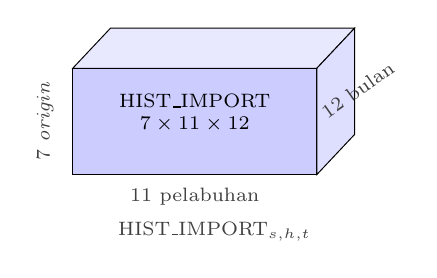
\begin{tikzpicture}[
    every node/.style={font=\scriptsize},
    front/.style={draw=black, line width=0.35pt},
    topface/.style={draw=black, line width=0.35pt},
    sideface/.style={draw=black, line width=0.35pt},
    axislabel/.style={font=\scriptsize, text=black!75},
    tensorlabel/.style={font=\bfseries\scriptsize, align=center}
]
\filldraw[front, fill=blue!20] (0,0) rectangle (3.1,1.35);
\filldraw[topface, fill=blue!9] (0,1.35) -- (0.48,1.86) -- (3.58,1.86) -- (3.1,1.35) -- cycle;
\filldraw[sideface, fill=blue!13] (3.1,0) -- (3.58,0.51) -- (3.58,1.86) -- (3.1,1.35) -- cycle;
\node[tensorlabel] at (1.55,0.78) {$\mathrm{HIST\_IMPORT}$\\$7 \times 11 \times 12$};
\node[axislabel] at (1.55,-0.28) {11 pelabuhan};
\node[axislabel, rotate=90] at (-0.35,0.68) {7 \textit{origin}};
\node[axislabel, rotate=35] at (3.62,1.08) {12 bulan};
\node[axislabel] at (1.8,-0.72) {$\mathrm{HIST\_IMPORT}_{s,h,t}$};
\end{tikzpicture}
\end{center}
Dengan bentuk tersebut, \textit{input} yang dibaca ALNS bukan satu vektor abstrak, melainkan parameter berindeks yang sudah memiliki arti operasional. Representasi tensor sebagai \textit{state} solusi baru dijelaskan pada bagian implementasi algoritma. Pada bagian pra-pemrosesan ini, matriks dan tensor berperan sebagai bahan baku numerik yang membatasi dan menilai solusi.

\begin{table}[H]
\centering
\caption{Keluaran pra-pemrosesan dan fungsi implementatifnya}
\label{tab:output_preprocessing}
\scriptsize
\begin{tabularx}{\textwidth}{@{}p{0.24\textwidth}p{0.14\textwidth}p{0.20\textwidth}X@{}}
\toprule
\textbf{Keluaran} & \textbf{Dimensi} & \textbf{Sumber aktif} & \textbf{Fungsi dalam ALNS} \\
\midrule
\texttt{DEMAND} / $D_{i,t}$ & $38 \times 12$ & Neraca Kedelai 2024 & Menghitung kebutuhan, \textit{shortage}, \textit{service rate}, dan bobot alokasi. \\
\texttt{PROD\_CAP} / $Cap^{PROD}_{k,t}$ & $20 \times 12$ & Produksi tahunan dan musim panen & Membatasi aliran lokal. \\
\texttt{IMP\_CAP\_NORMAL} / $Cap^{IMP}_{s,t}$ & $7 \times 12$ & Bobot impor 2022--2025 & Membatasi impor reguler. \\
\texttt{PORT\_THRU\_CAP} / $Cap^{PORT}_{h,t}$ & $11 \times 12$ & Bobot impor non-bandara 2022--2025 & Membatasi total \textit{inflow/outflow} pelabuhan. \\
\texttt{HIST\_IMPORT} & $7 \times 11 \times 12$ & Bobot impor 2024 & \textit{Seed} impor pada solusi awal. \\
\texttt{C\_PURCH} / $C^{PURCH}_{s}$ & $7$ & Bobot dan nilai dolar impor & Biaya pembelian impor reguler. \\
\texttt{C\_SHIP} / $C^{SHIP}_{k,i}$ & $20 \times 38$ & Koordinat dan \textit{seed} biaya & Biaya pengiriman lokal. \\
\texttt{C\_DIST} / $C^{DIST}_{h,i}$ & $11 \times 38$ & Koordinat dan \textit{seed} biaya & Biaya distribusi pelabuhan ke provinsi. \\
\texttt{C\_TRANS} / $C^{TRANS}_{i,j}$ & $38 \times 38$ & Koordinat dan \textit{seed} biaya & Biaya transfer antarprovinsi. \\
\texttt{SAFETY\_STOCK} / $SS_i$ & $38$ & Turunan \texttt{DEMAND} & Menentukan status aman provinsi. \\
\texttt{PROV\_STOR\_CAP} / $Cap^{STOR}_i$ & $38$ & Turunan \texttt{DEMAND} & Membatasi inventori provinsi. \\
\bottomrule
\end{tabularx}
\end{table}

\subsection{Ringkasan Skala \textit{Instance} Utama}

Setelah mekanik pada \ref{tab:preprocess_mechanics} dijalankan, \textit{instance} utama memiliki skala numerik seperti pada \ref{tab:preprocessing_snapshot}. Tabel ini bukan hasil optimasi, melainkan ringkasan parameter sebelum ALNS membentuk dan memperbaiki solusi.

\begin{table}[H]
\centering
\caption{Ringkasan skala hasil pra-pemrosesan pada \textit{instance} utama}
\label{tab:preprocessing_snapshot}
\scriptsize
\begin{tabularx}{\textwidth}{@{}p{0.25\textwidth}p{0.16\textwidth}rX@{}}
\toprule
\textbf{Parameter siap pakai} & \textbf{Bentuk} & \textbf{Total nasional} & \textbf{Makna skala} \\
\midrule
\texttt{DEMAND} & $38 \times 12$ & 2.409.333,82 ton & Kebutuhan kedelai nasional selama 12 bulan. \\
\texttt{PROD\_CAP} & $20 \times 12$ & 240.982,89 ton & Batas maksimum pasokan lokal dari seluruh sentra produksi. \\
\texttt{IMP\_CAP\_NORMAL} & $7 \times 12$ & 4.431.650,51 ton & Batas atas pasokan impor reguler setelah \textit{buffer} kapasitas. \\
\texttt{PORT\_THRU\_CAP} & $11 \times 12$ & 5.920.088,93 ton & Batas atas \textit{throughput} pelabuhan setelah \textit{buffer} kapasitas. \\
\texttt{SAFETY\_STOCK} & $38$ & 220.855,60 ton & Target stok aman seluruh provinsi. \\
\texttt{PROV\_STOR\_CAP} & $38$ & 803.111,27 ton & Batas kapasitas simpan seluruh provinsi. \\
\bottomrule
\end{tabularx}
\end{table}

\subsection{Dari Parameter ke MILP dan ALNS}

Hubungan antara hasil pra-pemrosesan, model MILP, dan implementasi ALNS diringkas pada \ref{tab:preprocess_to_milp_alns}. Tabel ini menjadi jembatan pembacaan: parameter yang sama muncul sebagai simbol pada model matematis dan sebagai array pada algoritma.

\begin{table}[H]
\centering
\caption{Hubungan keluaran pra-pemrosesan dengan MILP dan ALNS}
\label{tab:preprocess_to_milp_alns}
\scriptsize
\begin{tabularx}{\textwidth}{@{}p{0.20\textwidth}p{0.36\textwidth}X@{}}
\toprule
\textbf{Parameter} & \textbf{Terlihat di MILP sebagai} & \textbf{Terlihat di ALNS/hasil sebagai} \\
\midrule
$D_{i,t}$ & Neraca inventori dan perhitungan \textit{shortage}. & Permintaan untuk \textit{repair}, \textit{service rate}, inventori, dan \textit{shortage}. \\
$Cap^{PROD}_{k,t}$ & Kendala kapasitas produksi lokal. & Batas aliran lokal pada solusi awal, Tabu Search, dan PRS import-to-local. \\
$Cap^{IMP}_{s,t}$ & Kendala kuota impor reguler per \textit{origin}. & Batas volume impor dan aktivasi kontrak \textit{origin}. \\
$Cap^{PORT}_{h,t}$ & Kendala \textit{throughput} pelabuhan. & Batas \textit{inflow/outflow} pelabuhan dan utilisasi pelabuhan. \\
$HIST\_IMPORT_{s,h,t}$ & Data pembentuk kandidat awal. & \textit{Seed} impor awal sebelum ALNS memperbaiki rute. \\
$C^{PURCH}$, $C^{SHIP}$, $C^{DIST}$, $C^{TRANS}$ & Komponen fungsi objektif biaya. & Skor biaya kandidat dan \textit{breakdown} biaya. \\
$SS_i$, $Cap^{STOR}_i$ & Kendala stok aman dan kapasitas gudang. & Status stok aman, inventori, dan kelayakan transfer. \\
\bottomrule
\end{tabularx}
\end{table}

% ─────────────────────────────────────────────────────────────────────────────
\section{Implementasi Model dan Algoritma}

\subsection{Representasi Solusi pada Implementasi}

Mengacu pada kerangka LNS/ALNS, solusi tidak harus direpresentasikan sebagai satu vektor pipih. Solusi dapat dipahami sebagai himpunan variabel keputusan yang sebagian elemennya dihancurkan dan dibangun kembali oleh operator \textit{destroy} dan \textit{repair}, sebagaimana pola umum LNS pada \ref{alg:lns} dan ALNS pada \ref{alg:alns}. Pada penelitian ini, bentuk konseptual pada \ref{tab:representasi_bab3} diimplementasikan sebagai empat tensor aliran utama. Setiap tensor menyimpan volume kedelai dalam ton, dengan tiga arah pembacaan: node asal, node tujuan, dan periode bulan.

Dalam implementasi ALNS, himpunan nilai solusi yang sedang dipegang oleh algoritma disebut \textit{state}. Istilah \textit{state} digunakan karena ALNS tidak hanya perlu menyimpan nilai variabel keputusan utama, tetapi juga kondisi turunan yang muncul setelah aliran tersebut dihitung ulang. Dengan kata lain, \textit{state} adalah ``foto lengkap'' dari satu kandidat solusi pada suatu iterasi: berapa aliran lokal, impor, distribusi, dan transfernya; berapa inventori dan \textit{shortage} yang dihasilkan; serta apakah indikator kebijakan seperti aktivasi impor atau kelayakan transfer terpenuhi. Di dalam kode, \textit{state} ini direpresentasikan oleh kelas \texttt{SoybeanState}.

Perbedaannya dengan objek \texttt{Problem} pada bagian pra-pemrosesan adalah sebagai berikut: \texttt{Problem} menyimpan soal optimasi yang tetap, sedangkan \texttt{State} menyimpan jawaban sementara untuk soal tersebut. Karena itu, satu \texttt{Problem} dapat dievaluasi dengan banyak \texttt{State} berbeda selama proses ALNS.

Karena itu, perlu dibedakan antara \textbf{tensor keputusan utama} dan \textbf{komponen turunan \textit{state}}. Empat tensor \(X^{loc}\), \(X^{imp}\), \(X^{dist}\), dan \(X^{trns}\) adalah variabel aliran utama yang langsung dibuka, dikurangi, ditambah, atau dirute ulang oleh operator ALNS. Sementara itu, \(inv\), \(sh\), \(safe\), \(w\), \(y\) tetap disimpan di dalam \textit{state}, tetapi bukan blok aliran utama yang biasanya diacak langsung oleh operator. Komponen tersebut dihitung ulang dari tensor aliran untuk mengetahui konsekuensi fisik dan kebijakan dari solusi, seperti inventori akhir, kekurangan pasokan, status stok aman, kelayakan transfer, aktivasi impor reguler.

Dengan demikian, komponen keputusan utama dari satu \textit{state} ALNS pada penelitian ini direpresentasikan sebagai
\[
S_{\text{flow}} =
\left\{
X^{loc},\,
X^{imp},\,
X^{dist},\,
X^{trns}
\right\}.
\]
Sementara itu, \textit{state} lengkap yang disimpan oleh program juga memuat komponen turunan:
\[
S =
\left(
S_{\text{flow}},
inv,\,
sh,\,
safe,\,
w,\,
y
\right).
\]
Keempat tensor tersebut memiliki dimensi sebagai berikut:
\[
\begin{aligned}
X^{loc}  &\in \mathbb{R}_{+}^{20 \times 38 \times 12},
&
X^{imp}  &\in \mathbb{R}_{+}^{7 \times 11 \times 12},
&
X^{dist} &\in \mathbb{R}_{+}^{11 \times 38 \times 12},
&
X^{trns} &\in \mathbb{R}_{+}^{38 \times 38 \times 12}.
\end{aligned}
\]
Notasi tersebut berarti bahwa satu elemen tensor selalu memiliki makna operasional. Sebagai contoh, \(x^{imp}_{s,h,t}\) menyatakan aliran impor dari \textit{origin} \(s\) ke pelabuhan \(h\) pada bulan \(t\), sedangkan \(x^{dist}_{h,i,t}\) menyatakan distribusi dari pelabuhan \(h\) ke provinsi \(i\) pada bulan \(t\). Bentuk ini lebih mudah dibaca dibandingkan satu vektor pipih karena setiap indeks langsung menunjukkan asal, tujuan, dan periode keputusan.

\begin{figure}[H]
\centering
\resizebox{0.96\textwidth}{!}{%
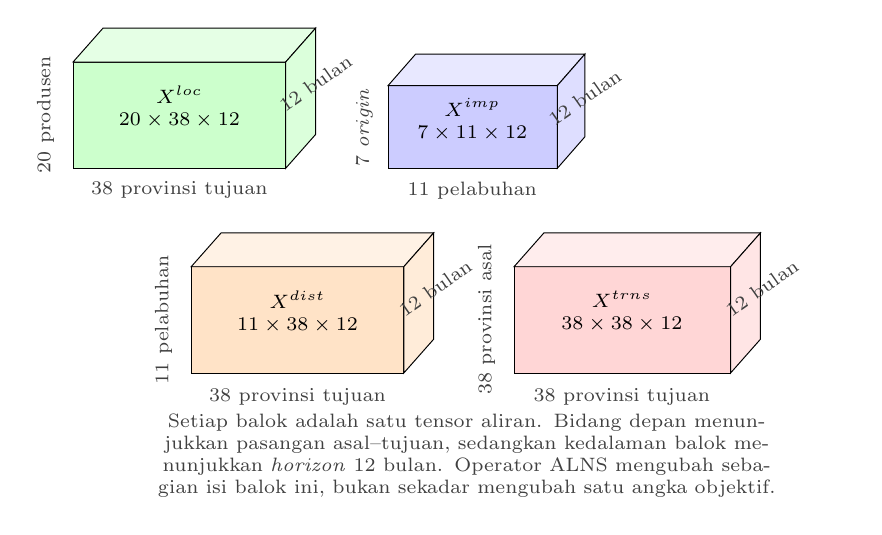
\begin{tikzpicture}[
    every node/.style={font=\scriptsize},
    front/.style={draw=black, line width=0.35pt},
    topface/.style={draw=black, line width=0.35pt},
    sideface/.style={draw=black, line width=0.35pt},
    axislabel/.style={font=\scriptsize, text=black!75},
    tensorlabel/.style={font=\bfseries\scriptsize, align=center},
    note/.style={font=\scriptsize, align=center, text=black!75}
]

% tensor cuboids: front face = origin x destination, depth = 12 months
\filldraw[front, fill=green!20] (0,0) rectangle (2.7,1.35);
\filldraw[topface, fill=green!10] (0,1.35) -- (0.38,1.78) -- (3.08,1.78) -- (2.7,1.35) -- cycle;
\filldraw[sideface, fill=green!14] (2.7,0) -- (3.08,0.43) -- (3.08,1.78) -- (2.7,1.35) -- cycle;
\node[tensorlabel] at (1.35,0.78) {$X^{loc}$\\$20 \times 38 \times 12$};
\node[axislabel] at (1.35,-0.28) {38 provinsi tujuan};
\node[axislabel, rotate=90] at (-0.35,0.68) {20 produsen};
\node[axislabel, rotate=35] at (3.08,1.08) {12 bulan};

\filldraw[front, fill=blue!20] (4.0,0) rectangle (6.15,1.05);
\filldraw[topface, fill=blue!9] (4.0,1.05) -- (4.35,1.45) -- (6.5,1.45) -- (6.15,1.05) -- cycle;
\filldraw[sideface, fill=blue!13] (6.15,0) -- (6.5,0.4) -- (6.5,1.45) -- (6.15,1.05) -- cycle;
\node[tensorlabel] at (5.07,0.62) {$X^{imp}$\\$7 \times 11 \times 12$};
\node[axislabel] at (5.07,-0.28) {11 pelabuhan};
\node[axislabel, rotate=90] at (3.7,0.52) {7 \textit{origin}};
\node[axislabel, rotate=35] at (6.5,0.9) {12 bulan};


\filldraw[front, fill=orange!22] (1.5,-2.6) rectangle (4.2,-1.25);
\filldraw[topface, fill=orange!10] (1.5,-1.25) -- (1.88,-0.82) -- (4.58,-0.82) -- (4.2,-1.25) -- cycle;
\filldraw[sideface, fill=orange!15] (4.2,-2.6) -- (4.58,-2.17) -- (4.58,-0.82) -- (4.2,-1.25) -- cycle;
\node[tensorlabel] at (2.85,-1.82) {$X^{dist}$\\$11 \times 38 \times 12$};
\node[axislabel] at (2.85,-2.9) {38 provinsi tujuan};
\node[axislabel, rotate=90] at (1.15,-1.92) {11 pelabuhan};
\node[axislabel, rotate=35] at (4.6,-1.52) {12 bulan};

\filldraw[front, fill=red!16] (5.6,-2.6) rectangle (8.35,-1.25);
\filldraw[topface, fill=red!7] (5.6,-1.25) -- (5.98,-0.82) -- (8.73,-0.82) -- (8.35,-1.25) -- cycle;
\filldraw[sideface, fill=red!10] (8.35,-2.6) -- (8.73,-2.17) -- (8.73,-0.82) -- (8.35,-1.25) -- cycle;
\node[tensorlabel] at (6.97,-1.82) {$X^{trns}$\\$38 \times 38 \times 12$};
\node[axislabel] at (6.97,-2.9) {38 provinsi tujuan};
\node[axislabel, rotate=90] at (5.25,-1.92) {38 provinsi asal};
\node[axislabel, rotate=35] at (8.75,-1.52) {12 bulan};

\node[note, text width=9.6cm] at (5.0,-3.65)
{Setiap balok adalah satu tensor aliran. Bidang depan menunjukkan pasangan asal--tujuan, sedangkan kedalaman balok menunjukkan \textit{horizon} 12 bulan. Operator ALNS mengubah sebagian isi balok ini, bukan sekadar mengubah satu angka objektif.};

\end{tikzpicture}
}
\caption{Struktur tensor aliran pada representasi solusi ALNS.}
\label{fig:tensor-solusi-alns}
\end{figure}

Secara matematis, representasi tensor tersebut sebenarnya bisa ditulis sebagai satu vektor keputusan besar. Jika seluruh elemen pada empat tensor aliran diratakan dan disusun berurutan, maka diperoleh
\[
x =
\begin{bmatrix}
\operatorname{vec}\left(X^{loc}\right) \\
\operatorname{vec}\left(X^{imp}\right) \\
\operatorname{vec}\left(X^{dist}\right) \\
\operatorname{vec}\left(X^{trns}\right)
\end{bmatrix}
\in \mathbb{R}_{+}^{32388}.
\]
Jumlah 32388 elemen tersebut berasal dari
\[
\begin{aligned}
32388
&=
(20 \times 38 \times 12)
+ (7 \times 11 \times 12)
+ (11 \times 38 \times 12)
+ (38 \times 38 \times 12).
\end{aligned}
\]
Dengan kata lain, representasi tensor dan representasi vektor pipih memuat informasi yang sama. Permasalahannya, bentuk vektor pipih menyembunyikan arti setiap elemen. Sebagai contoh, satu elemen pada vektor \(x\) tidak langsung terlihat apakah ia merepresentasikan impor dari \textit{origin} ke pelabuhan, distribusi dari pelabuhan ke provinsi, produksi lokal, atau transfer antarprovinsi. Untuk membaca elemen tersebut, diperlukan fungsi indeks tambahan yang memetakan posisi vektor kembali ke bentuk asal--tujuan--bulan.

Hal ini membuat representasi vektor pipih kurang informatif untuk menjelaskan cara kerja ALNS pada masalah rantai pasok ini. Operator \textit{destroy} dan \textit{repair} tidak sekadar memilih angka ke-\(r\) dari vektor \(x\), tetapi memilih bagian solusi yang memiliki makna operasional, misalnya bulan tertentu, provinsi dengan \textit{shortage}, pelabuhan yang menjadi \textit{bottleneck}, atau jalur transfer antarprovinsi. Oleh karena itu, bentuk vektor \(x \in \mathbb{R}_{+}^{32388}\) tetap sah secara matematis, tetapi representasi tensor dipertahankan karena lebih jelas untuk menunjukkan struktur keputusan dan perubahan yang dilakukan oleh ALNS.

Pada metode optimasi yang bekerja dengan operasi numerik umum, satu vektor pipih sering terasa lebih sederhana karena algoritma dapat langsung mengubah angka-angka di dalam vektor tersebut. Namun, ALNS tidak mencari solusi dengan mengubah angka secara bebas satu per satu. Kekuatan ALNS justru berasal dari operator yang memahami struktur masalah: bagian solusi yang dianggap bermasalah dibuka, lalu dibangun kembali dengan aturan yang mempertimbangkan kapasitas, biaya, neraca pasokan, dan hubungan antar-node. Karena itu, menyimpan solusi sebagai tensor aliran membantu operator memilih dan memperbaiki bagian solusi yang tepat. Misalnya, operator dapat menghapus seluruh aliran pada bulan tertentu, membuka ulang alokasi menuju provinsi yang masih kekurangan, atau mengurangi ketergantungan pada pelabuhan yang terlalu padat. \textbf{Jika} semua keputusan hanya dipandang sebagai \textbf{vektor satu dimensi}, operasi-operasi tersebut \textbf{tetap mungkin dilakukan}, \textbf{tetapi} harus diawali dengan \textbf{pemetaan indeks} yang \textbf{rumit}.

\begin{figure}[H]
\centering
\resizebox{!}{3.5cm}{%
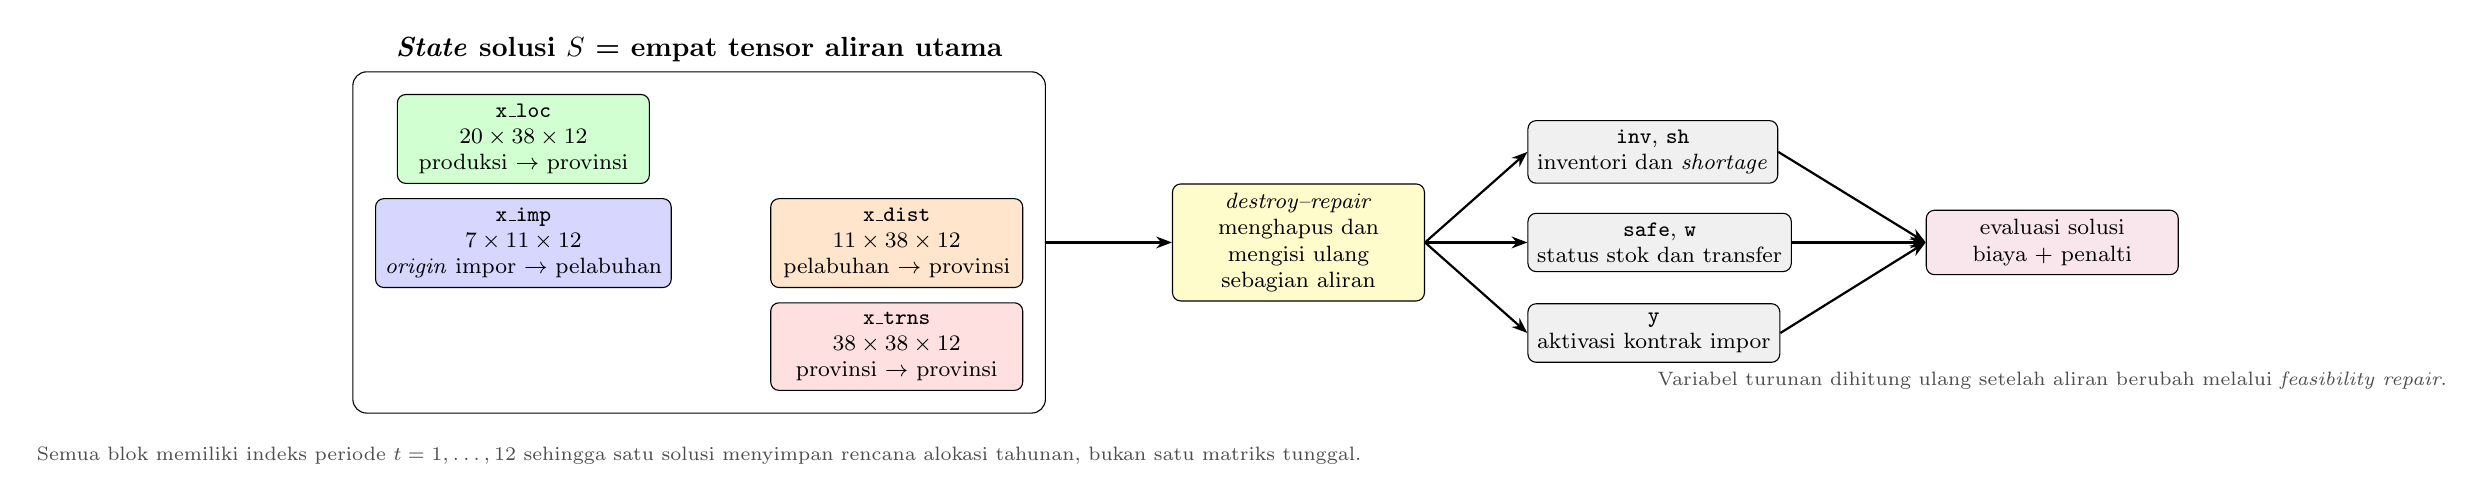
\begin{tikzpicture}[
    every node/.style={font=\footnotesize},
    flowblock/.style={rectangle, draw=black, rounded corners=3pt, minimum width=3.2cm, minimum height=0.78cm, align=center},
    derivedblock/.style={rectangle, draw=black, rounded corners=3pt, minimum width=2.7cm, minimum height=0.68cm, align=center, fill=gray!12},
    groupbox/.style={rectangle, draw=black, rounded corners=5pt, inner sep=8pt},
    arrow/.style={-{Stealth[length=2mm]}, thick},
    note/.style={font=\scriptsize, align=center, text=black!70}
]

% Main state container
\node[flowblock, fill=green!18] (xloc) at (0, 1.8) {\texttt{x\_loc}\\$20 \times 38 \times 12$\\produksi $\rightarrow$ provinsi};
\node[flowblock, fill=blue!16, below=0.18cm of xloc] (ximp) {\texttt{x\_imp}\\$7 \times 11 \times 12$\\\textit{origin} impor $\rightarrow$ pelabuhan};
\node[flowblock, fill=orange!20, right=1.25cm of ximp] (xdist) {\texttt{x\_dist}\\$11 \times 38 \times 12$\\pelabuhan $\rightarrow$ provinsi};
\node[flowblock, fill=red!12, below=0.18cm of xdist] (xtrns) {\texttt{x\_trns}\\$38 \times 38 \times 12$\\provinsi $\rightarrow$ provinsi};

\begin{scope}[on background layer]
    \node[groupbox, fit=(xloc) (ximp) (xdist) (xtrns), label={[font=\bfseries]above:\textit{State} solusi $S$ = empat tensor aliran utama}] (statebox) {};
\end{scope}

% Operators and repair
\node[flowblock, fill=yellow!20, right=1.6cm of statebox, text width=2.9cm] (ops) {\textit{destroy--repair}\\menghapus dan mengisi ulang sebagian aliran};
\node[derivedblock, right=1.3cm of ops, yshift=1.15cm] (inv) {\texttt{inv}, \texttt{sh}\\inventori dan \textit{shortage}};
\node[derivedblock, right=1.3cm of ops] (policy) {\texttt{safe}, \texttt{w}\\status stok dan transfer};
\node[derivedblock, right=1.3cm of ops, yshift=-1.15cm] (binary) {\texttt{y}\\aktivasi kontrak impor};
\node[flowblock, fill=purple!10, right=1.7cm of policy, text width=2.5cm] (obj) {evaluasi solusi\\biaya + penalti};

\draw[arrow] (statebox.east) -- (ops.west);
\draw[arrow] (ops.east) -- (inv.west);
\draw[arrow] (ops.east) -- (policy.west);
\draw[arrow] (ops.east) -- (binary.west);
\draw[arrow] (inv.east) -- (obj.west);
\draw[arrow] (policy.east) -- (obj.west);
\draw[arrow] (binary.east) -- (obj.west);

\node[note, below=0.3cm of statebox] {Semua blok memiliki indeks periode $t=1,\ldots,12$ sehingga satu solusi menyimpan rencana alokasi tahunan, bukan satu matriks tunggal.};
\node[note, below=1.1cm of obj] {Variabel turunan dihitung ulang setelah aliran berubah melalui \textit{feasibility repair}.};

\end{tikzpicture}
}
\caption{Visualisasi \textit{state} solusi ALNS sebagai empat tensor aliran utama.}
\label{fig:representasi-solusi-alns}
\end{figure}

\ref{fig:representasi-solusi-alns} menunjukkan empat blok aliran utama merupakan bagian solusi yang dimodifikasi operator, sedangkan inventori, kekurangan pasokan, dan indikator kebijakan dihitung ulang dari aliran tersebut

Pada implementasi program, seluruh keputusan aliran dan variabel turunan yang dihitung dari aliran tersebut akan disimpan. Ini dilakukan agar operator ALNS dapat mengubah sebagian aliran solusi secara langsung, sedangkan fungsi objektif dan mekanisme kelayakan dapat menghitung kembali konsekuensinya terhadap biaya, inventori, kekurangan pasokan, dan aturan kebijakan.

Komponen solusi yang disimpan dirangkum pada \ref{tab:soybean_state_representation}. Tabel tersebut memuat dua kelompok. Lima array pertama merupakan tensor aliran utama yang dimodifikasi oleh operator, sedangkan komponen lainnya merupakan kondisi turunan yang dihitung ulang setelah aliran berubah. Dengan demikian, ketika naskah menyebut ``empat tensor'', yang dimaksud adalah empat tensor keputusan utama, bukan seluruh isi \textit{state}.

\begin{table}[H]
\centering
\small
\caption{Representasi solusi pada kelas \texttt{SoybeanState}}
\label{tab:soybean_state_representation}
\begin{tabularx}{\textwidth}{@{}>{\RaggedRight\arraybackslash}p{0.18\textwidth}>{\centering\arraybackslash}p{0.22\textwidth}>{\RaggedRight\arraybackslash}p{0.50\textwidth}@{}}
\toprule
\textbf{Komponen} & \textbf{Dimensi} & \textbf{Makna implementatif} \\
\midrule
\texttt{x\_loc} & $20 \times 38 \times 12$ & Aliran kedelai lokal dari sentra produksi ke provinsi tujuan. \\
\texttt{x\_imp} & $7 \times 11 \times 12$ & Aliran impor reguler dari \textit{origin} impor ke pelabuhan. \\
\texttt{x\_dist} & $11 \times 38 \times 12$ & Distribusi kedelai dari pelabuhan ke provinsi. \\
\texttt{x\_trns} & $38 \times 38 \times 12$ & Transfer kedelai antarprovinsi. \\
\texttt{inv} & $38 \times 12$ & Inventori akhir provinsi setelah permintaan bulan tersebut dipenuhi. \\
\texttt{sh} & $38 \times 12$ & Kekurangan pasokan provinsi pada bulan tertentu. \\
\texttt{safe} & $38 \times 12$ & Indikator terpenuhinya stok aman provinsi. \\
\texttt{w} & $38 \times 12$ & Indikator provinsi layak menjadi asal transfer. \\
\texttt{y} & $7 \times 12$ & Indikator aktivasi kontrak impor reguler per \textit{origin} dan bulan. \\
\bottomrule
\end{tabularx}
\end{table}

Tampilan konkret \textit{state} pada artefak hasil optimasi ditunjukkan pada \ref{tab:state_snapshot_json}. Tabel ini memperlihatkan bahwa \textit{output} ALNS bukan satu angka objektif saja, melainkan komponen-komponen tensor solusi dan variabel turunan yang dapat ditelusuri kembali ke sumber, pelabuhan, provinsi, dan bulan.

\begin{table}[H]
\centering
\caption{\textit{Snapshot state} pada \texttt{hasil/optimization\_result.json}}
\label{tab:state_snapshot_json}
\scriptsize
\begin{tabularx}{\textwidth}{@{}p{0.15\textwidth}p{0.17\textwidth}rrX@{}}
\toprule
\textbf{Komponen} & \textbf{Dimensi} & \textbf{Initial} & \textbf{Best} & \textbf{Makna pembacaan} \\
\midrule
\texttt{x\_loc} & $20 \times 38 \times 12$ & 200.214,89 & 240.982,89 & Total pasokan lokal yang dialokasikan selama 12 bulan. \\
\texttt{x\_imp} & $7 \times 11 \times 12$ & 2.672.007,60 & 2.279.321,79 & Total impor reguler dari \textit{origin} ke pelabuhan. \\
\texttt{x\_dist} & $11 \times 38 \times 12$ & 2.672.007,60 & 2.279.321,79 & Seluruh inflow pelabuhan keluar lagi sebagai distribusi. \\
\texttt{x\_trns} & $38 \times 38 \times 12$ & 0,00 & 0,00 & Transfer antarprovinsi tidak terpakai pada solusi utama ini. \\
\texttt{inv} & $38 \times 12$ & 3.764.174,14 & 1.060.684,45 & Total inventori akhir provinsi lintas bulan. \\
\texttt{sh} & $38 \times 12$ & 11.851,95 & 0,00 & Shortage awal berhasil dihilangkan pada solusi terbaik. \\
\texttt{y} & $7 \times 12$ & 40 & 48 & Banyaknya aktivasi \textit{origin} impor reguler lintas bulan. \\
\bottomrule
\end{tabularx}
\end{table}

Tabel tersebut menunjukkan bahwa bentuk implementasi mengikuti struktur tensor. Setiap komponen aliran disimpan sebagai blok terpisah agar operator ALNS dapat langsung membaca konteksnya. Dengan cara ini, kode dapat mengubah \(x^{imp}_{s,h,t}\) sebagai aliran impor dari \textit{origin} \(s\) ke pelabuhan \(h\), atau \(x^{dist}_{h,i,t}\) sebagai distribusi dari pelabuhan \(h\) ke provinsi \(i\), tanpa harus menghitung posisi elemen tersebut dalam vektor pipih berdimensi 32388.

Ruang pencarian adalah seluruh kemungkinan nilai pada keempat tensor aliran tersebut. Namun, tidak seluruh kombinasi nilai dapat menghasilkan rencana rantai pasok yang valid. Misalnya, menaikkan impor pada suatu pelabuhan tanpa menaikkan distribusi keluar akan membuat pelabuhan seolah-olah menyimpan stok, padahal model memperlakukan pelabuhan sebagai titik \textit{throughput}. Jadi, kedelai yang masuk ke pelabuhan harus keluar lagi sebagai distribusi pada bulan yang sama. Oleh karena itu, setiap perubahan solusi harus diikuti perhitungan ulang kondisi turunan.

Nilai objektif solusi dihitung sebagai penjumlahan biaya produksi dan pengiriman lokal, pembelian impor distribusi pelabuhan, transfer antarprovinsi, penyimpanan provinsi, biaya tetap aktivasi impor. Nilai tersebut kemudian ditambah penalti apabila terjadi pelanggaran terhadap target yang ditentukan di awal, yaitu total \textit{shortage}, batas ketergantungan impor, batas minimal penyerapan lokal, dan batas minimal inventori.

\subsection{Pembentukan Solusi Awal (\textit{Initial Solution})}

Solusi awal dirancang sebagai titik mulai pencarian yang masih dekat dengan pola aliran aktual. Rancangannya ditunjukkan pada \ref{alg:initial_solution_concept}, sedangkan bentuk di program diringkas pada \ref{tab:initial_solution_construction}. Pada tabel tersebut, \(x^{loc}\), \(x^{imp}\), \(x^{dist}\), dan \(x^{trns}\) adalah tensor aliran utama sesuai di \ref{tab:soybean_state_representation} dan \ref{fig:tensor-solusi-alns}. Sementara itu, \(inv\), \(sh\), \(safe\), \(w\), dan \(y\) adalah nilai turunan yang dihitung setelah aliran awal terbentuk.

Solusi awal dibuat dari pola impor historis, bukan dari alokasi kosong. Hasilnya adalah rencana awal yang sudah berisi impor, pasokan lokal, dan distribusi keluar pelabuhan sebelum ALNS mulai memperbaiki alokasi. Bagian ini meneruskan hasil pra-pemrosesan pada \ref{tab:output_preprocessing}. Nilai \(D\) berasal dari contoh tabel permintaan pada \ref{tab:preprocessing_demand_matrix_example}, \(Cap^{PROD}\) dari \ref{tab:preprocessing_prod_cap_matrix_example}, \(Cap^{PORT}\) dari \ref{tab:preprocessing_port_cap_matrix_example}, dan \(HIST\_IMPORT\) dari \ref{tab:preprocessing_hist_import_tensor_example}. Parameter tersebut kemudian mengisi tensor \textit{state} yang bentuknya ditunjukkan pada \ref{fig:tensor-solusi-alns} dan diringkas pada \ref{tab:soybean_state_representation}.

\begin{table}[H]
\centering
\caption{Alur pembentukan solusi awal ALNS}
\label{tab:initial_solution_construction}
\scriptsize
\renewcommand{\arraystretch}{1.5}
\begin{tabularx}{\textwidth}{@{}p{0.08\textwidth}p{0.23\textwidth}p{0.18\textwidth}X@{}}
\toprule
\textbf{No.} & \textbf{Data masuk} & \textbf{Array diisi} & \textbf{Aturan singkat} \\
\midrule
1 & $HIST\_IMPORT$, $Cap^{PORT}$ & $x^{imp}_{s,h,t}$ & Ambil impor historis \textit{origin}--pelabuhan--bulan, lalu batasi dengan $0{,}95Cap^{PORT}_{h,t}$. \\
2 & $Cap^{PROD}$, $D$ & $x^{loc}_{k,i,t}$ & Kirim produksi lokal ke provinsi produsennya sendiri, maksimum $\min(Cap^{PROD}_{k,t},0{,}5D_{i_k,t})$. \\
3 & $x^{imp}$, $D$, $C^{DIST}$ & $x^{dist}_{h,i,t}$ & Gunakan permintaan sebagai bobot awal pembagian impor. Jika total permintaan lebih besar dari impor yang masuk, bobot tersebut diskalakan turun. Untuk setiap provinsi, coba pelabuhan termurah lebih dulu. \\
4 & -- & $x^{trns}_{i,j,t}$ & Transfer antarprovinsi dibuat nol pada awal pencarian. \\
5 & Semua aliran awal & $inv,sh,safe,w,y$ & Jalankan \textit{feasibility repair} untuk menghitung inventori, kekurangan, status stok, dan aktivasi impor. \\
\bottomrule
\end{tabularx}
\renewcommand{\arraystretch}{1}
\end{table}

Aturan pada \ref{tab:initial_solution_construction} dapat dibaca per bagian sebagai berikut.

\[
\begin{aligned}
\text{(a) } x^{imp}_{s,h,t}
&\leftarrow
\min\left(
\underbrace{HIST\_IMPORT_{s,h,t}}_{\substack{\text{impor}\\\text{historis}}},
\underbrace{0{,}95Cap^{PORT}_{h,t}}_{\substack{\text{batas}\\\text{pelabuhan}}}
\right).
\end{aligned}
\]
\noindent Artinya impor awal mengikuti data historis \textit{origin}--pelabuhan--bulan, tetapi tidak boleh langsung memenuhi seluruh kapasitas pelabuhan.

\[
\begin{aligned}
\text{(b) } x^{loc}_{k,i_k,t}
&\leftarrow
\min\left(
\underbrace{Cap^{PROD}_{k,t}}_{\substack{\text{kapasitas}\\\text{produksi}}},
\underbrace{0{,}5D_{i_k,t}}_{\substack{\text{setengah}\\\text{permintaan}}}
\right).
\end{aligned}
\]
\noindent Artinya produksi lokal awal dikirim ke provinsi produsennya sendiri, tetapi tidak langsung menutup seluruh permintaannya.

\[
\begin{aligned}
\text{(c) } I_t
&=
\underbrace{\sum_{s,h}x^{imp}_{s,h,t}}_{\substack{\text{total impor}\\\text{masuk pelabuhan}}},
\qquad
Q_t
=
\underbrace{\sum_i D_{i,t}}_{\substack{\text{total permintaan}\\\text{provinsi}}}.
\end{aligned}
\]
\noindent Artinya \(I_t\) adalah jumlah impor yang benar-benar masuk ke semua pelabuhan pada bulan \(t\), sedangkan \(Q_t\) adalah total permintaan provinsi pada bulan yang sama.

\[
\begin{aligned}
\text{(d) } \mathrm{target}_{i,t}
&\leftarrow
\begin{cases}
\underbrace{D_{i,t}}_{\text{permintaan provinsi}},
& \text{jika } Q_t \le I_t,\\[0.55em]
\underbrace{D_{i,t}}_{\text{permintaan provinsi}}
\underbrace{\dfrac{I_t}{Q_t}}_{\text{faktor skala}},
& \text{jika } Q_t > I_t.
\end{cases}
\end{aligned}
\]
\noindent Artinya jika total permintaan tidak lebih besar dari impor yang masuk, target tiap provinsi tetap sama dengan permintaannya. Jika total permintaan lebih besar, semua target dikalikan faktor yang sama, yaitu \(I_t/Q_t\). Dengan begitu, total distribusi tidak melebihi impor yang masuk, tetapi proporsi antarprovinsi tetap mengikuti permintaan.

\[
\begin{aligned}
\text{(e) } x^{dist}_{h,i,t}
&\leftarrow
\underbrace{\text{alokasi } \mathrm{target}_{i,t}}_{\substack{\text{jatah}\\\text{provinsi}}}
\text{ dari }
\underbrace{\arg\min_h C^{DIST}_{h,i}}_{\substack{\text{pelabuhan}\\\text{termurah}}}.
\end{aligned}
\]
\noindent Artinya impor yang sudah masuk pelabuhan dibagikan ke provinsi, dimulai dari pelabuhan dengan biaya distribusi terendah.

\[
\begin{aligned}
\text{(f) } x^{trns}_{i,j,t}
&\leftarrow
\underbrace{0}_{\substack{\text{belum ada}\\\text{transfer}}}.
\end{aligned}
\]
\noindent Artinya solusi awal belum menggunakan transfer antarprovinsi; transfer baru muncul jika operator ALNS membentuknya.

\[
\begin{aligned}
\text{(g) } (inv,sh,safe,w,y)
&\leftarrow
\underbrace{
\text{\textit{feasibility repair}}(x^{loc},x^{imp},x^{dist},x^{trns})
}_{\substack{\text{hitung ulang}\\\text{kondisi turunan}}}.
\end{aligned}
\]
\noindent Artinya setelah aliran awal terbentuk, inventori, kekurangan, status stok, aktivasi, dan kelayakan transfer dihitung ulang agar solusi awal dapat dievaluasi.

Tiga hal perlu diperhatikan. Pertama, \(HIST\_IMPORT\) hanya berisi negara asal, pelabuhan, dan bulan; data tersebut belum memiliki tujuan provinsi. Karena itu, \(x^{dist}\) dibentuk dari permintaan provinsi dan biaya distribusi pelabuhan ke provinsi. Kedua, kekurangan pasokan yang tersisa pada solusi awal tidak langsung ditutup dengan impor baru; bagian ini menjadi ruang perbaikan ALNS. Ketiga, setelah solusi awal terbentuk, parameter \(\epsilon_3\) dikunci pada total produksi lokal solusi awal, sehingga ALNS tidak boleh menurunkan penyerapan lokal di bawah titik awal tersebut.

Perlu ditegaskan bahwa \textit{Initial} pada hasil program dan \textit{dashboard} berarti solusi awal ALNS, bukan stok awal fisik sebelum \textit{horizon} perencanaan dimulai. Pada implementasi saat ini, perhitungan neraca inventori dimulai dari persediaan pembuka nol di setiap provinsi, kemudian inventori bulan ke-$t$ dihitung dari pasokan masuk, transfer, dan permintaan pada bulan tersebut. Karena itu, inventori yang terlihat pada solusi awal merupakan inventori akhir bulan hasil konstruksi \textit{historical seeding}, bukan data stok pembuka yang berdiri sendiri.

\subsection{Siklus Interaksi ALNS dengan \textit{State}, Kendala, dan Objektif}

Sebelum masuk ke notasi iterasi, hubungan antara \texttt{Problem}, \texttt{State}, dan proses ALNS diringkas pada \ref{fig:problem_state_alns_flow}. Gambar ini memperinci interaksi konseptual pada \ref{fig:alns_interaction_concept} dan \ref{tab:alns_interaction_concept}: data dan aturan tetap berada pada \texttt{Problem}, sedangkan ALNS bekerja dengan mengubah \texttt{State} sebagai kandidat solusi.

\begin{figure}[H]
\centering
\resizebox{0.98\textwidth}{!}{%
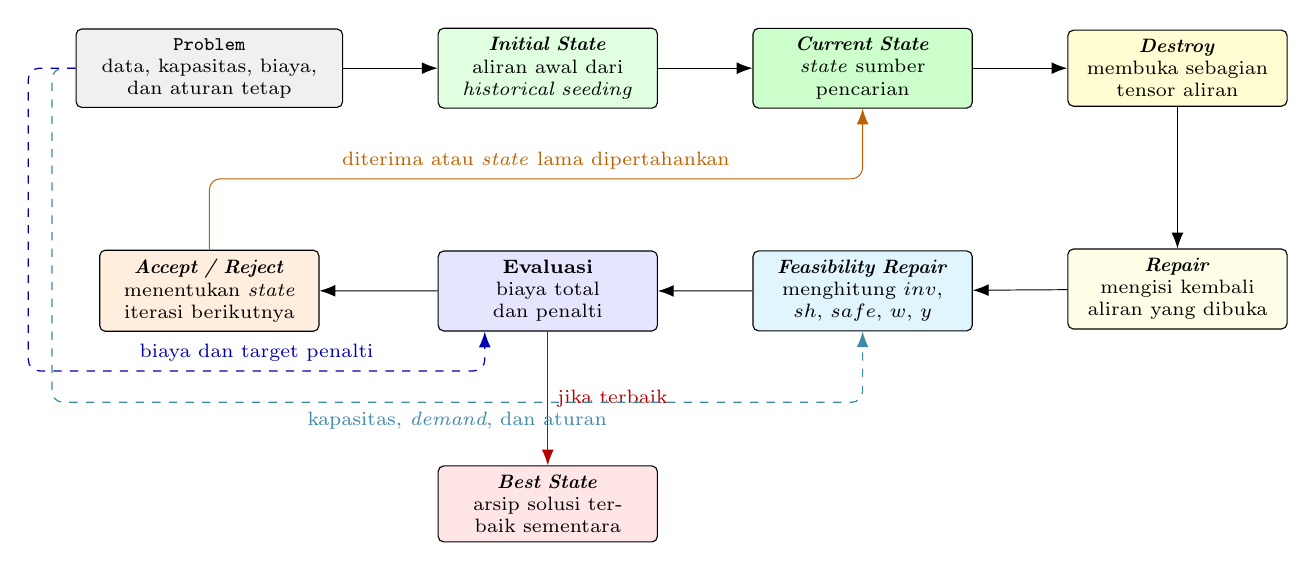
\begin{tikzpicture}[
    node distance=1.8cm and 1.2cm,
    box/.style={
        rectangle,
        draw=black,
        rounded corners=2pt,
        align=center,
        minimum width=2.65cm,
        minimum height=0.78cm,
        font=\scriptsize,
        text width=2.55cm
    },
    widebox/.style={
        rectangle,
        draw=black,
        rounded corners=2pt,
        align=center,
        minimum width=3.25cm,
        minimum height=0.82cm,
        font=\scriptsize,
        text width=3.15cm
    },
    arrow/.style={-{Latex[length=2mm]}, line width=0.35pt},
    dashedarrow/.style={-{Latex[length=2mm]}, dashed, line width=0.45pt}
]

\node[widebox, fill=gray!12] (problem) {\textbf{\texttt{Problem}}\\data, kapasitas, biaya, dan aturan tetap};
\node[box, fill=green!12, right=of problem] (initial) {\textbf{\textit{Initial State}}\\aliran awal dari \textit{historical seeding}};
\node[box, fill=green!20, right=of initial] (current) {\textbf{\textit{Current State}}\\\textit{state} sumber pencarian};
\node[box, fill=yellow!18, right=of current] (destroy) {\textbf{\textit{Destroy}}\\membuka sebagian tensor aliran};

\node[box, fill=yellow!10, below=1.8cm of destroy] (repair) {\textbf{\textit{Repair}}\\mengisi kembali aliran yang dibuka};
\node[box, fill=cyan!12, below=1.8cm of current] (feas) {\textbf{\textit{Feasibility Repair}}\\menghitung $inv$, $sh$, $safe$, $w$, $y$};
\node[box, fill=blue!10, below=1.8cm of initial] (eval) {\textbf{Evaluasi}\\biaya total dan penalti};
\node[box, fill=orange!13, below=1.8cm of problem] (accept) {\textbf{\textit{Accept / Reject}}\\menentukan \textit{state} iterasi berikutnya};

\node[box, fill=red!10, below=1.7cm of eval] (best) {\textbf{\textit{Best State}}\\arsip solusi terbaik sementara};

\draw[arrow] (problem) -- (initial);
\draw[arrow] (initial) -- (current);
\draw[arrow] (current) -- (destroy);
\draw[arrow] (destroy) -- (repair);
\draw[arrow] (repair) -- (feas);
\draw[arrow] (feas) -- (eval);
\draw[arrow] (eval) -- (accept);

\draw[arrow, rounded corners=4pt, draw=orange!75!black] (accept.north) -- +(0, 0.9cm) -| (current.south) node[pos=0.25, above, font=\scriptsize, text=orange!75!black] {diterima atau \textit{state} lama dipertahankan};
\draw[arrow, draw=red!70!black] (eval) -- node[right, font=\scriptsize, text=red!70!black] {jika terbaik} (best);

\draw[dashedarrow, rounded corners=4pt, draw=cyan!65!black] (problem.west) -- +(-0.3cm,0) |- ([yshift=-0.9cm]feas.south) node[pos=0.75, below, font=\scriptsize, text=cyan!65!black] {kapasitas, \textit{demand}, dan aturan} -- (feas.south);
\draw[dashedarrow, rounded corners=4pt, draw=blue!70!black] (problem.west) -- +(-0.6cm,0) |- ([yshift=-0.5cm, xshift=-0.8cm]eval.south) node[pos=0.75, above, font=\scriptsize, text=blue!70!black] {biaya dan target penalti} -- ([xshift=-0.8cm]eval.south);

\end{tikzpicture}
}
\caption{Alur hubungan \texttt{Problem}, \texttt{State}, dan siklus perubahan solusi pada ALNS.}
\label{fig:problem_state_alns_flow}
\end{figure}

Dengan sudut pandang tensor, satu iterasi ALNS dapat dipahami sebagai proses mengubah \textit{state} solusi saat ini \(S_k\) menjadi kandidat baru. Algoritma tidak mengubah model MILP secara simbolik pada setiap iterasi, tetapi mengubah nilai pada tensor aliran yang merepresentasikan solusi. Dalam kode, \textit{state} ini tampil sebagai objek \texttt{SoybeanState}, yaitu kumpulan array \texttt{x\_loc}, \texttt{x\_imp}, \texttt{x\_dist}, dan \texttt{x\_trns}. Model MILP berperan sebagai kerangka evaluasi: nilai aliran dibaca sebagai nilai variabel keputusan, kemudian neraca, kapasitas, indikator kebijakan, biaya, dan penalti dihitung ulang untuk menilai kualitas kandidat.

Kegunaan \textit{state} adalah menjadi objek kerja utama selama pencarian. Operator \textit{destroy} menerima satu \textit{state}, membuka sebagian alirannya, lalu operator \textit{repair} menghasilkan \textit{state} kandidat baru. Setelah itu, \textit{feasibility repair} melengkapi kembali kondisi turunan sehingga kandidat dapat dievaluasi secara adil. Dengan struktur ini, ALNS dapat menyalin, memodifikasi, menerima, menolak, dan menyimpan solusi terbaik tanpa harus membangun ulang formulasi MILP dari awal pada setiap iterasi.

Alur perubahan satu solusi dapat diringkas sebagai
\[
S_k
\rightarrow
S'_k
\rightarrow
S''_k
\rightarrow
S^{cand}_k
\rightarrow
S_{k+1}.
\]
Tahap \textit{destroy} menghasilkan \(S'_k\) dengan menghapus atau mengurangi sebagian isi tensor aliran. Tahap \textit{repair} menghasilkan \(S''_k\) dengan mengisi kembali bagian yang dibuka tersebut. Setelah itu, \textit{feasibility repair} menghasilkan \(S^{cand}_k\), yaitu kandidat yang telah dihitung ulang agar konsisten dengan kapasitas, neraca aliran, inventori, \textit{shortage}, dan aturan kebijakan.

Secara ringkas, proses pembentukan kandidat dapat ditulis sebagai
\[
S^{cand}_k =
\Pi_{\mathcal{F}}
\left(
R_b
\left(
D_a(S_k)
\right)
\right),
\]
dengan \(D_a\) sebagai operator \textit{destroy}, \(R_b\) sebagai operator \textit{repair}, dan \(\Pi_{\mathcal{F}}\) sebagai proses \textit{feasibility repair}. Kandidat kemudian diterima atau ditolak melalui mekanisme penerimaan ALNS:
\[
S_{k+1}
=
\begin{cases}
S^{cand}_k, & \text{jika kandidat diterima},\\
S_k, & \text{jika kandidat ditolak}.
\end{cases}
\]

Pada implementasi, operasi tersebut tidak dilakukan dengan memilih indeks vektor secara acak satu per satu. Operator ALNS bekerja pada bagian tensor yang memiliki makna operasional, misalnya seluruh aliran pada bulan tertentu, seluruh aliran menuju provinsi yang mengalami \textit{shortage}, atau seluruh aliran yang melalui pelabuhan \textit{bottleneck}. Dengan demikian, ALNS bekerja atas satu \textit{state} solusi \(S\), tetapi perubahan dilakukan pada blok-blok tensor yang berkaitan langsung dengan keputusan rantai pasok.

\begin{figure}[H]
\centering
\fbox{%
\begin{minipage}{0.92\textwidth}
\small
\textbf{Interaksi satu iterasi ALNS pada implementasi}

\vspace{0.25em}
\[
S_{\text{current}}
\rightarrow
S_{\text{partial}}
\rightarrow
S_{\text{candidate}}
\rightarrow
S_{\text{repaired}}
\rightarrow
f(S_{\text{repaired}})
\rightarrow
S_{\text{current}} \text{ atau } S_{\text{best}}
\]

\vspace{0.25em}
\begin{tabularx}{\linewidth}{@{}p{0.18\linewidth}X@{}}
\textbf{Repair} & Mengubah $S_{\text{partial}}$ menjadi $S_{\text{candidate}}$ dengan mengisi kembali kebutuhan yang terbuka menggunakan aturan konstruksi tertentu. \\
\textbf{\textit{Feasibility repair}} & Mengubah $S_{\text{candidate}}$ menjadi $S_{\text{repaired}}$ dengan menghitung ulang konsekuensi fisik dan indikator kebijakan. \\
\textbf{Evaluasi} & Fungsi objektif membaca $S_{\text{repaired}}$ untuk menghitung biaya total dan penalti pelanggaran. \\
\end{tabularx}
\end{minipage}}
\caption{Alur teknis interaksi ALNS dengan \textit{state} solusi dan model evaluasi.}
\label{fig:alns_state_interaction}
\end{figure}

Umpan balik diberikan melalui tiga mekanisme: penerimaan kandidat oleh \textit{Simulated Annealing} sesuai prinsip pada \ref{eq:sa_accept_incumbent}, pembaruan bobot operator berdasarkan kualitas kandidat, dan intensifikasi lokal pada solusi terbaik. Pemilihan operator mengikuti peluang roulette pada \ref{eq:alns_roulette}, sedangkan skor dan pembaruan bobot mengikuti mekanisme pada \ref{eq:alns_reward} dan \ref{eq:alns_weight_update}.

\begin{algorithm}[H]\footnotesize
\caption{Siklus Interaksi ALNS dengan \textit{State} Solusi}
\label{alg:alns_state_interaction}
\KwIn{\textit{Problem instance}, portofolio operator \textit{destroy}, portofolio operator \textit{repair}, jumlah iterasi}
\KwOut{\textit{State} solusi terbaik $S_{\text{best}}$ dan riwayat evaluasi}
Bentuk $S_{\text{current}}$ dari solusi awal berbasis data historis\;
Jalankan \textit{feasibility repair} pada $S_{\text{current}}$\;
Hitung objektif awal dan tetapkan $S_{\text{best}} \leftarrow S_{\text{current}}$\;
Inisialisasi bobot operator \textit{destroy} dan \textit{repair}\;
\For{iterasi ke-$r = 1,\ldots,R$}{
    Pilih satu operator \textit{destroy} dan satu operator \textit{repair} berdasarkan bobot adaptif\;
    $S_{\text{partial}} \leftarrow$ \textit{destroy}$(S_{\text{current}})$\;
    $S_{\text{candidate}} \leftarrow$ \textit{repair}$(S_{\text{partial}})$\;
    Jalankan \textit{feasibility repair} pada $S_{\text{candidate}}$\;
    Hitung biaya dan penalti $S_{\text{candidate}}$\;
    \tcp{Penerimaan SA: bandingkan dengan $S_{\text{current}}$, bukan $S_{\text{best}}$}
    \eIf{$c(S_{\text{candidate}}) \leq c(S_{\text{current}})$}{
        $S_{\text{current}} \leftarrow S_{\text{candidate}}$\;
        \eIf{$c(S_{\text{candidate}}) < c(S_{\text{best}})$}{
            $S_{\text{best}} \leftarrow S_{\text{candidate}}$\;
            Beri skor $\omega_1$ (\textit{new global best})\;
        }{
            Beri skor $\omega_2$ (\textit{better than incumbent})\;
        }
    }{
        \eIf{SA menerima kandidat yang lebih buruk}{
            $S_{\text{current}} \leftarrow S_{\text{candidate}}$\;
            Beri skor $\omega_3$ (\textit{accepted by SA})\;
        }{
            Beri skor $\omega_4$ (\textit{rejected})\;
        }
    }
    Perbarui bobot operator: $\rho \leftarrow \lambda\rho + (1-\lambda)\psi$, dengan lantai minimum $\rho_{\min}$\;
    \If{konfigurasi intensifikasi lokal aktif}{
        Terapkan \textit{Tabu Search} atau PRS adapted pada $S_{\text{best}}$\;
        Jalankan \textit{feasibility repair} dan terima hasil lokal hanya jika objektif membaik\;
    }
    Simpan riwayat objektif, biaya, penalti, \textit{shortage}, dan penggunaan operator\;
}
\KwRet{$S_{\text{best}}$}
\end{algorithm}
\ref{tab:alns_cycle_detail} menunjukkan apa yang berubah pada setiap langkah. Tabel ini juga menjelaskan hubungan antara ALNS dan model MILP: MILP menyediakan struktur keputusan, batasan, dan fungsi evaluasi, sedangkan ALNS menyediakan cara mencari kombinasi nilai variabel yang baik tanpa menyelesaikan seluruh model secara eksak.

\begin{table}[H]
\centering
\caption{Detail perubahan \textit{state} pada siklus ALNS}
\label{tab:alns_cycle_detail}
\small
\renewcommand{\arraystretch}{1.38}
\begin{tabularx}{\textwidth}{@{}c p{0.18\textwidth}p{0.31\textwidth}X@{}}
\toprule
\textbf{No.} & \textbf{Langkah (urut)} & \textbf{Array atau komponen yang berubah} & \textbf{Makna interaksi dengan model} \\
\midrule
1 & Solusi awal & \texttt{x\_imp}, \texttt{x\_loc}, \texttt{x\_dist}. & Nilai awal variabel keputusan dibentuk dari pola data historis dan kapasitas fisik. \\
2 & \textit{Repair} & Array aliran yang kosong atau berkurang setelah \textit{destroy}. & Kebutuhan yang terbuka diisi ulang dengan pilihan sumber, pelabuhan, atau transfer yang lebih menjanjikan. \\
3 & \textit{Feasibility repair} & \texttt{inv}, \texttt{sh}, \texttt{safe}, \texttt{w}, \texttt{y}, serta aliran yang melampaui batas. & Kandidat dinormalkan agar neraca barang, kapasitas, aktivasi impor, dan aturan transfer terbaca konsisten. \\
4 & Evaluasi objektif & Komponen biaya dan penalti. & Model membaca \textit{state} sebagai satu solusi lengkap, lalu menghasilkan nilai objektif untuk perbandingan. \\
5 & Penerimaan SA & \textit{current state}. & Kandidat yang lebih buruk masih dapat diterima dengan probabilitas tertentu agar pencarian tidak cepat terjebak. \\
6 & \textit{Update} bobot & Bobot operator \textit{destroy} dan \textit{repair}. & Operator yang menghasilkan solusi baik dipilih lebih sering pada iterasi berikutnya. \\
7 & TS atau PRS adapted & \textit{best state}. & Solusi terbaik diperbaiki dengan perubahan lokal yang kecil dan terarah, kemudian dievaluasi ulang. \\
\bottomrule
\end{tabularx}
\end{table}
Peran operator \textit{destroy} dan \textit{repair} tidak sama. Operator \textit{destroy} menentukan bagian solusi mana yang dibuka kembali, sedangkan operator \textit{repair} menentukan cara bagian tersebut dibangun ulang. Detail mekanisme yang digunakan pada kode diringkas pada \ref{tab:destroy_operator_detail}, \ref{tab:repair_operator_detail}, dan \ref{alg:feasibility_repair_code}.

\begin{table}[H]
\centering
\caption{Detail mekanisme \textit{destroy operator} pada implementasi ALNS}
\label{tab:destroy_operator_detail}
\scriptsize
\renewcommand{\arraystretch}{2}
\begin{tabularx}{\textwidth}{@{}p{0.24\textwidth}p{0.43\textwidth}X@{}}
\toprule
\textbf{Operator} & \textbf{Mekanisme pemilihan area} & \textbf{Perubahan pada \textit{state}} \\
\midrule
\texttt{destroy\_random\_temporal} & Ambil $\rho \sim U(0{,}15,0{,}35)$, lalu pilih $k=\max(1,\lfloor \rho |T| \rfloor)$ bulan secara acak. & Nolkan \texttt{x\_loc}, \texttt{x\_imp}, \texttt{x\_dist}, dan \texttt{x\_trns} pada bulan terpilih. \\
\texttt{destroy\_cost\_based} & Hitung biaya bulanan dari aliran lokal, impor reguler, dan distribusi pelabuhan; pilih $k$ bulan dengan biaya tertinggi. & Nolkan \texttt{x\_loc}, \texttt{x\_imp}, \texttt{x\_dist}, dan \texttt{x\_trns} pada bulan mahal tersebut. \\
\texttt{destroy\_shortage\_based} & Jika total \textit{shortage} nol, \textit{fallback} ke \textit{random temporal}; jika tidak, pilih pasangan provinsi-bulan dengan $sh_{i,t}$ terbesar dan buka jendela 5 bulan di sekitarnya. & Nolkan pasokan lokal, distribusi pelabuhan, serta transfer masuk/keluar untuk provinsi tersebut pada jendela waktu terpilih. \\
\texttt{destroy\_geographic} & Pilih satu kluster wilayah secara acak dan pilih $k$ bulan acak dengan $\rho \sim U(0{,}15,0{,}35)$. & Nolkan pasokan lokal, distribusi pelabuhan, dan transfer masuk/keluar untuk semua provinsi dalam kluster pada bulan terpilih. \\
\texttt{destroy\_bottleneck\_port} & Pilih pelabuhan dengan utilisasi terbesar, dihitung dari total \texttt{x\_imp} sepanjang \textit{horizon}. & Nolkan impor reguler dan distribusi keluar dari pelabuhan tersebut. \\
\texttt{destroy\_relatedness} & Pilih provinsi \textit{pivot} acak; hitung \textit{relatedness} $0{,}6$ kemiripan \textit{demand} + $0{,}4$ kesamaan kluster; pilih provinsi paling terkait dan beberapa bulan acak. & Nolkan pasokan lokal, distribusi pelabuhan, dan transfer masuk/keluar untuk provinsi terkait pada bulan terpilih. \\
\bottomrule
\end{tabularx}
\renewcommand{\arraystretch}{1}
\end{table}

\begin{table}[H]
\centering
\caption{Detail mekanisme \textit{repair operator} pada implementasi ALNS}
\label{tab:repair_operator_detail}
\scriptsize
\renewcommand{\arraystretch}{2}
\begin{tabularx}{\textwidth}{@{}p{0.24\textwidth}p{0.43\textwidth}X@{}}
\toprule
\textbf{Operator} & \textbf{Mekanisme pengisian} & \textbf{Catatan kode} \\
\midrule
\texttt{repair\_greedy} & Untuk tiap bulan, hitung sisa kapasitas produksi, impor, dan pelabuhan; isi defisit provinsi berdasarkan urutan defisit relatif terbesar. Sumber dipilih berdasarkan biaya lokal atau rute impor termurah. & Jika rasio impor sudah mencapai/melewati \texttt{EPS\_IMPORT\_DEP}, biaya \textit{sort-key} impor ditambah penalti besar sehingga sumber lokal didahulukan. \\
\texttt{repair\_regret} & Hitung \textit{regret} tiap provinsi sebagai selisih biaya sumber terbaik dan kedua terbaik; provinsi dengan \textit{regret} terbesar diisi lebih dulu. & Jika sumber lokal terbaik lebih murah dari impor termurah, gunakan lokal; sisa defisit diisi dari \textit{origin} CIF termurah melalui pelabuhan pertama yang masih memiliki kapasitas. \\
\texttt{repair\_balanced} & Isi provinsi ber-\textit{demand} tinggi lebih dulu; pilih lokal jika lebih murah, lalu isi impor secara \textit{round-robin}. & Setiap \textit{origin} impor dibatasi maksimum $0{,}6D_{i,t}$ untuk provinsi tersebut; jika impor tidak cukup, \textit{fallback} ke lokal. \\
\texttt{repair\_transfer\_focused} & Fase 1: pilih 10 calon donor dari skor $0{,}6$ akses pelabuhan murah + $0{,}4$ produksi lokal, lalu \textit{seed} inventori bulan 0--2. Fase 1.5: surplus awal boleh diarahkan ke provinsi kritis. Fase 2: bulan 3--11, transfer surplus dari donor \textit{eligible} ke provinsi defisit. & Transfer mendahulukan donor satu kluster lalu biaya transfer termurah; \textit{eligibility} donor tetap divalidasi ulang oleh \textit{feasibility repair}. \\
\bottomrule
\end{tabularx}
\renewcommand{\arraystretch}{1}
\end{table}

\begin{algorithm}[H]\footnotesize
\caption{\textit{Feasibility repair} pada implementasi}
\label{alg:feasibility_repair_code}
\KwIn{\textit{State} kandidat $S$ berisi tensor aliran; \textit{instance} masalah $P$}
\KwOut{\textit{State} $S$ dengan $inv$, $sh$, $safe$, $y$, $w$, dan penalti infeasibilitas yang diperbarui}
$penalty \leftarrow 0$; $inv^{prev}_i \leftarrow 0,\ \forall i \in I$\;
\For{$t = 1,\ldots,|T|$}{
    $portIn_h \leftarrow \sum_s x^{imp}_{s,h,t},\ \forall h \in H$\;

    \ForEach{$h \in H$ dengan $portIn_h > Cap^{PORT}_{h,t}$}{
        $\gamma_h \leftarrow Cap^{PORT}_{h,t}/portIn_h$\;
        $x^{imp}_{s,h,t} \leftarrow \gamma_h x^{imp}_{s,h,t},\ \forall s$\;
    }

    \ForEach{$h \in H$}{
        $a_h \leftarrow \sum_s x^{imp}_{s,h,t}$;\quad
        $b_h \leftarrow \sum_i x^{dist}_{h,i,t}$\;
        \eIf{$a_h \le 0$}{
            $x^{dist}_{h,i,t} \leftarrow 0,\ \forall i$\;
        }{
            \eIf{$b_h = 0$}{
                Bagi $a_h$ merata ke provinsi dalam \texttt{PORT\_SERV}$(h)$ sebagai nilai awal $x^{dist}_{h,i,t}$\;
            }{
                $x^{dist}_{h,i,t} \leftarrow (a_h/b_h)x^{dist}_{h,i,t},\ \forall i$\;
            }
        }
    }

    $\Delta_i \leftarrow \sum_k x^{loc}_{k,i,t}+\sum_h x^{dist}_{h,i,t}+\sum_j x^{trns}_{j,i,t}-\sum_j x^{trns}_{i,j,t},\ \forall i$\;
    $raw_i \leftarrow inv^{prev}_i+\Delta_i-D_{i,t}$\;
    $sh_{i,t} \leftarrow \max(0,-raw_i)$; \quad $inv_{i,t} \leftarrow \max(0,raw_i)$\;

    \ForEach{$i \in I$ dengan $inv_{i,t} > Cap^{STOR}_i$}{
        $\beta_i \leftarrow \max\{0,\min(1,1-(inv_{i,t}-Cap^{STOR}_i)/\max(\Delta_i,10^{-9}))\}$\;
        Kalikan $x^{loc}_{k,i,t}$, $x^{dist}_{h,i,t}$, dan $x^{trns}_{j,i,t}$ dengan $\beta_i$\;
        Hitung ulang $inv_{i,t}$ dan $sh_{i,t}$ untuk provinsi $i$, lalu batasi $inv_{i,t} \le Cap^{STOR}_i$\;
    }

    $safe_{i,t} \leftarrow \mathbb{1}[inv_{i,t}\ge SS_i],\ \forall i$\;

    Ulangi normalisasi pelabuhan: untuk setiap $h$, paksa $\sum_i x^{dist}_{h,i,t}=\sum_s x^{imp}_{s,h,t}$\;
    Hitung ulang final $\Delta_i$, $raw_i$, $sh_{i,t}$, $inv_{i,t}$, dan $safe_{i,t}$\;
    $y_{s,t} \leftarrow \mathbb{1}[\sum_h x^{imp}_{s,h,t}>0],\ \forall s$\;
    $inv^{prev}_i \leftarrow inv_{i,t},\ \forall i$\;
}

$w_{i,t} \leftarrow 0,\ \forall i,t$\;
\For{$t = 4,\ldots,|T|$}{
    $w_{i,t} \leftarrow safe_{i,t-1}\land safe_{i,t-2}\land safe_{i,t-3},\ \forall i$\;
}
\ForEach{$(i,t)$ dengan $w_{i,t}=0$ dan $\sum_j x^{trns}_{i,j,t}>0$}{
    \eIf{$t \le 3$ dan seluruh transfer keluar $i$ menuju provinsi kritis}{
        Pertahankan transfer awal tersebut\;
    }{
        $penalty \leftarrow penalty+\sum_j x^{trns}_{i,j,t}$\;
        $x^{trns}_{i,j,t}\leftarrow 0,\ \forall j$\;
    }
}
$S.\_penalty \leftarrow penalty$; hapus \textit{cache} objektif \textit{state}\;
\KwRet{$S$}
\end{algorithm}
\noindent Dengan urutan ini, objektif menilai angka yang bukan mentah hasil operator, tetapi menilai \textit{state} yang telah dinormalisasi agar konsisten dengan neraca barang, kapasitas fisik, status kebijakan, dan aturan transfer.

\subsection{Konfigurasi yang Dievaluasi}
Bagian ini membahas perbandingan tiga konfigurasi \textit{baseline} pada \ref{tab:baseline_config}. Konfigurasi tersebut memiliki data \textit{input}, fungsi objektif, dan jumlah iterasi yang serupa, serta hanya dibedakan oleh intensifikasi lokal pasca proses \textit{destroy--repair}.

\begin{table}[H]
\centering
\caption{Konfigurasi \textit{baseline} yang dibandingkan}
\label{tab:config_compared_bab4}
\small
\begin{tabularx}{\textwidth}{@{}p{0.22\textwidth}p{0.28\textwidth}p{0.22\textwidth}X@{}}
\toprule
\textbf{Konfigurasi} & \textbf{Intensifikasi lokal} & \textbf{Jumlah \textit{run}} & \textbf{Peran dalam pembandingan} \\
\midrule
ALNS-TS & \textit{Tabu Search} substitusi impor-ke-lokal pada $S_{best}$. & 50 \textit{seed} $\times$ 500 iterasi & \textit{Baseline} ALNS dengan intensifikasi lokal klasik. \\
ALNS-PRS adapted & Gerakan lokal diskrit PRS-\textit{inspired} pada $S_{best}$. & 50 \textit{seed} $\times$ 500 iterasi & Kandidat konfigurasi utama untuk eksperimen lanjutan. \\
ALNS-only & Tanpa intensifikasi lokal tambahan. & 50 \textit{seed} $\times$ 500 iterasi & \textit{Baseline} untuk melihat kontribusi intensifikasi. \\
\bottomrule
\end{tabularx}
\end{table}

\noindent Selain menghasilkan tabel dan gambar untuk naskah, implementasi juga mengekspor artefak keluaran yang dapat diperiksa ulang. Artefak tersebut dirangkum pada \ref{tab:artefak_keluaran}. Pemisahan ini penting karena \textit{dashboard} dan pembahasan membaca hasil dari artefak yang sama, bukan menjalankan ulang \textit{solver} dengan data berbeda.

\begin{table}[H]
\centering
\caption{Artefak keluaran implementasi}
\label{tab:artefak_keluaran}
\small
\renewcommand{\arraystretch}{1.25}
\begin{tabularx}{\textwidth}{@{}p{0.365\textwidth}p{0.32\textwidth}X@{}}
\toprule
\textbf{Artefak} & \textbf{Dihasilkan oleh} & \textbf{Isi dan fungsi} \\
\midrule
\texttt{hasil/optimization\_result.json} & \texttt{run\_optimization.py} & \textit{Handoff} utama berisi konfigurasi, \textit{instance} \texttt{Problem}, \textit{state initial/best}, metrik, histori konvergensi, dan \textit{breakdown} biaya/penalti. \\
\texttt{hasil/*.csv} dan \texttt{hasil/*.png} & \texttt{run\_optimization.py} & Ringkasan dan visualisasi \textit{single run} konfigurasi terpilih. \\
\texttt{multi\_hasil/summary.csv} dan gambar pembanding & \texttt{run\_experiments\_multi.py} & Hasil \textit{baseline} 3 konfigurasi $\times$ 50 \textit{seed} $\times$ 500 iterasi. \\
\texttt{scenario\_hasil/summary.csv} dan \texttt{scenario\_comparison.png} & \texttt{run\_scenarios\_best\_model.py} & Hasil 16 skenario \textit{what-if}, masing-masing 10 \textit{seed}. \\
\texttt{dashboard/data.js} & \texttt{build\_dashboard.py} & Transformasi JSON hasil optimasi menjadi data statis untuk \textit{dashboard}. \\
\texttt{dashboard/index.html} & \textit{Dashboard} statis & Antarmuka pembacaan hasil tanpa menjalankan \textit{solver} ulang. \\
\bottomrule
\end{tabularx}
\renewcommand{\arraystretch}{1}
\end{table}

% ─────────────────────────────────────────────────────────────────────────────
\section{Evaluasi Performa Algoritma}

\subsection{Perbandingan Konfigurasi \textit{Baseline} ALNS}

\begin{figure}[H]
\centering

\includegraphics[width=0.85\textwidth]{multi_hasil/comparison_bar.png}
\caption{Perbandingan metrik \textit{comparison bar} pengaturan \textit{baseline} tiga konfigurasi ALNS, 50 \textit{seed}}
\label{fig:baseline_comparison_bar}
\end{figure}

\begin{figure}[H]
\centering

\includegraphics[width=0.85\textwidth]{multi_hasil/comparison_boxplot.png}
\caption{Perbandingan metrik \textit{boxplot} pengaturan \textit{baseline} tiga konfigurasi ALNS, 50 \textit{seed}}
\label{fig:baseline_comparison_box}
\end{figure}


Di \ref{fig:baseline_comparison_bar} dan \ref{fig:baseline_comparison_box} dapat dilihat bahwa ALNS-PRS mencapai rata-rata \textit{shortage} terendah, diikuti oleh ALNS, sedangkan ALNS-TS memiliki rata-rata \textit{shortage} yang lebih tinggi pada eksperimen aktif, lalu bisa dilihat kalau ALNS-only memiliki banyak \textit{outlier} dengan \textit{shortage} yang besar, diikuti oleh ALNS-TS yang memiliki \textit{outlier} besar juga meskipun tidak sebanyak sebelumnya, lalu ALNS-PRS memiliki \textit{shortage} yang sangat bagus dengan \textit{outlier shortage} satu-satunya hanya 4.96 ton. Perbandingan ini tidak hanya dibaca dari satu \textit{run}, tetapi dari 50 \textit{seed} untuk setiap konfigurasi.


\begin{table}[H]
\centering
\caption{Ringkasan Statistik Eksperimen \textit{Multi-Seed} (50 \textit{seed} $\times$ 500 iterasi)}
\label{tab:multi_seed}
\small
\begin{tabularx}{\textwidth}{@{}Xrrr@{}}
\toprule
\textbf{Metrik} & \textbf{ALNS-TS} & \textbf{ALNS-PRS adapted} & \textbf{ALNS-only} \\
\midrule
Mean $Z_{cost}$ (T Rp) & 23{,}79 & 23{,}84 & 24{,}00 \\
Std $Z_{cost}$ (T Rp) & 0{,}39 & 0{,}58 & 0{,}55 \\
Best $Z_{cost}$ (T Rp) & 23{,}33 & 23{,}27 & 23{,}36 \\
Worst $Z_{cost}$ (T Rp) & 25{,}44 & 26{,}61 & 25{,}91 \\
Mean \textit{shortage} (ton) & 22{,}28 & 0{,}10 & 16{,}32 \\
Worst \textit{shortage} (ton) & 386{,}34 & 4{,}96 & 444{,}30 \\
Mean \textit{service rate} (\%) & 99{,}9991 & 100{,}0000 & 99{,}9993 \\
Mean \textit{import dependency} (\%) & 90{,}398 & 90{,}451 & 90{,}491 \\
Mean produksi lokal (ton) & 240.979{,}87 & 240.040{,}76 & 240.509{,}98 \\
Avg \textit{runtime} (s/\textit{run}) & 66{,}32 & 30{,}47 & 10{,}70 \\
\bottomrule
\end{tabularx}
\end{table}

Pembacaan keputusan \textit{baseline} diringkas pada \ref{tab:baseline_decision_matrix}. ALNS-PRS adapted dipilih bukan karena paling kecil pada satu metrik saja, tetapi karena kombinasi \textit{shortage} rata-rata, \textit{worst shortage}, dan \textit{runtime}-nya paling seimbang untuk eksperimen lanjutan.

\begin{table}[H]
\centering
\caption{Matriks pembacaan pemilihan konfigurasi}
\label{tab:baseline_decision_matrix}
\small
\begin{tabularx}{\textwidth}{@{}p{0.22\textwidth}p{0.22\textwidth}p{0.22\textwidth}X@{}}
\toprule
\textbf{Kriteria} & \textbf{ALNS-TS} & \textbf{ALNS-PRS adapted} & \textbf{ALNS-only} \\
\midrule
\textit{Shortage} rata-rata & 22{,}28 ton & \textbf{0{,}10 ton} & 16{,}32 ton \\
\textit{Worst shortage} & 386{,}34 ton & \textbf{4{,}96 ton} & 444{,}30 ton \\
\textit{Runtime} rata-rata & 66{,}32 s/\textit{run} & 30{,}47 s/\textit{run} & \textbf{10{,}70 s/\textit{run}} \\
Catatan & Lambat dan masih memiliki \textit{outlier shortage}. & \textit{Shortage} paling stabil dengan \textit{runtime} menengah. & Cepat, tetapi \textit{shortage} lebih tidak stabil. \\
Keputusan & \textit{Baseline} pembanding. & \textbf{Dipakai untuk \textit{run} utama dan skenario.} & \textit{Baseline} cepat tanpa intensifikasi. \\
\bottomrule
\end{tabularx}
\end{table}

\subsection{Konvergensi Konfigurasi Terpilih}

\begin{figure}[H]
\centering

\includegraphics[width=0.95\textwidth]{multi_hasil/config_2_convergence.png}
\caption{Konvergensi konfigurasi ALNS-PRS adapted terpilih dengan tampilan \textit{best/average/worst} dari 50 \textit{seed}}
\label{fig:ALNS_PRS_convergence}
\end{figure}
\ref{fig:ALNS_PRS_convergence} menunjukkan algoritma ALNS-PRS sudah konvergen di iterasi ke-500 untuk kasus \textit{best/average/worst} 

\subsection{Analisis Bobot Operator}

Analisis operator dibaca sebagai diagnostik proses pencarian. Ringkasan histori operator pada \ref{tab:operator_history_summary} menunjukkan bahwa mayoritas kandidat ditolak, tetapi setiap konfigurasi tetap menghasilkan kandidat \textit{better} dan \textit{new best} selama iterasi.

\begin{table}[H]
\centering
\caption{Ringkasan \textit{outcome} operator \textit{baseline} dari \texttt{multi\_hasil/operator\_history.csv}}
\label{tab:operator_history_summary}
\small
\begin{tabular}{@{}lrrrr@{}}
\toprule
\textbf{Konfigurasi} & \textbf{\textit{Accepted}} & \textbf{\textit{Better}} & \textbf{\textit{New best}} & \textbf{\textit{Rejected}} \\
\midrule
ALNS-TS & 2.403 & 1.766 & 565 & 20.266 \\
ALNS-PRS adapted & 2.467 & 1.576 & 855 & 20.102 \\
ALNS-only & 2.475 & 1.386 & 1.171 & 19.968 \\
\bottomrule
\end{tabular}
\end{table}

\begin{table}[H]
\centering
\caption{Operator paling sering muncul pada histori \textit{baseline}}
\label{tab:operator_top_summary}
\small
\begin{tabularx}{\textwidth}{@{}p{0.20\textwidth}p{0.36\textwidth}X@{}}
\toprule
\textbf{Konfigurasi} & \textbf{\textit{Destroy} dominan} & \textbf{\textit{Repair} dominan} \\
\midrule
ALNS-TS & \textit{shortage-based}, \textit{geographic}, \textit{random-temporal} & \textit{greedy}, \textit{balanced}, \textit{transfer-focused} \\
ALNS-PRS adapted & \textit{shortage-based}, \textit{random-temporal}, \textit{geographic} & \textit{greedy}, \textit{balanced}, \textit{transfer-focused} \\
ALNS-only & \textit{shortage-based}, \textit{random-temporal}, \textit{relatedness} & \textit{greedy}, \textit{balanced}, \textit{transfer-focused} \\
\bottomrule
\end{tabularx}
\end{table}
\noindent Tabel ini berfungsi sebagai diagnostik proses, sedangkan pemilihan konfigurasi tetap mengikuti \ref{tab:baseline_decision_matrix}. Histori operator menjelaskan bahwa semua konfigurasi menjalankan pembelajaran operator adaptif pada ruang solusi yang sama.

\section{Hasil Optimasi}

Hasil optimasi pada bagian ini menggunakan konfigurasi terpilih berdasarkan evaluasi \textit{baseline}, yaitu ALNS-PRS adapted sesuai rancangan. Konfigurasi ini digunakan sebagai solusi utama karena hasil \textit{multi-seed} menunjukkan \textit{shortage} rata-rata dan \textit{worst shortage} paling rendah, \textit{runtime} lebih rendah dari konfigurasi yang lain.

\subsection{Representasi Rekomendasi Hasil Optimasi}

Hasil optimasi dibaca sebagai rencana alokasi pasokan 12 bulan. Bentuk keluaran utamanya ditunjukkan pada \ref{fig:hasil_to_dashboard_flow} yaitu array aliran menjadi keputusan, lalu diringkas menjadi metrik dan \textit{dashboard}.

\begin{figure}[H]
\centering
\fbox{%
\begin{minipage}{0.90\textwidth}
\footnotesize
\centering
\textbf{Tensor aliran hasil optimasi}\\
Pasokan lokal, impor ke pelabuhan, distribusi pelabuhan, dan transfer antarprovinsi.\\[0.35em]
$\downarrow$\\[-0.1em]
\textbf{Rencana operasional}\\
Menjawab sumber pasokan, rute, provinsi tujuan, bulan, dan tonase.\\[0.35em]
$\downarrow$\\[-0.1em]
\textbf{Artefak hasil}\\
JSON menyimpan \textit{state}, metrik, histori konvergensi, dan \textit{breakdown} biaya; CSV/PNG menyajikan tabel dan grafik.\\[0.35em]
$\downarrow$\\[-0.1em]
\textbf{\textit{Dashboard}}\\
Membaca artefak yang sama untuk inspeksi nasional, provinsi, dan pelabuhan.
\end{minipage}}
\caption{Bentuk keluaran hasil optimasi dari array aliran menjadi rekomendasi dan \textit{dashboard}}
\label{fig:hasil_to_dashboard_flow}
\end{figure}

\ref{tab:hasil_question_map} merangkum cara membaca keluaran tersebut. Tujuannya agar pembaca mengetahui variabel mana yang menjawab pertanyaan tertentu.

\begin{table}[H]
\centering
\caption{Peta pertanyaan terhadap keluaran model}
\label{tab:hasil_question_map}
\small
\begin{tabularx}{\textwidth}{@{}p{0.34\textwidth}p{0.23\textwidth}X@{}}
\toprule
\textbf{Pertanyaan pembaca} & \textbf{Variabel/artefak} & \textbf{Bentuk jawaban} \\
\midrule
Berapa kedelai lokal yang dikirim dari sentra produksi ke provinsi? & $x^{loc}_{k,i,t}$ & Tabel/visual alokasi lokal per produsen, provinsi tujuan, dan bulan. \\
Berapa impor dari tiap \textit{origin} dan lewat pelabuhan mana? & $x^{imp}_{s,h,t}$ & Aliran \textit{origin}--pelabuhan per bulan dan utilisasi kapasitas \textit{origin}. \\
Provinsi menerima impor dari pelabuhan mana? & $x^{dist}_{h,i,t}$ & Rute pelabuhan--provinsi, volume distribusi, dan biaya \textit{landed cost}. \\
Apakah ada redistribusi antarprovinsi? & $x^{trns}_{i,j,t}$ & Transfer provinsi asal--tujuan dan volume bulanan. \\
Apakah permintaan terpenuhi? & $sh_{i,t}$, \textit{service rate} & \textit{Shortage} provinsi/bulan dan \textit{service rate} nasional. \\
Apakah stok aman terpenuhi? & $inv_{i,t}$, $safe_{i,t}$ & Inventori akhir bulan, status aman, dan pelanggaran inventori. \\
\bottomrule
\end{tabularx}
\end{table}
\textit{Dashboard} nanti membaca artefak hasil optimasi yang sama dengan pembahasan sebelumnya. Contoh pertanyaan operasional yang dapat dijawab melalui \textit{dashboard} dirangkum pada \ref{tab:dashboard_operasional}; contoh tampilannya ditunjukkan pada \ref{fig:dashboard_prov} dan \ref{fig:dashboard_port}.

\begin{table}[H]
\centering
\caption{Contoh pembacaan rekomendasi operasional melalui \textit{dashboard} hasil optimasi}
\label{tab:dashboard_operasional}
\small
\begin{tabularx}{\textwidth}{@{}>{\RaggedRight\arraybackslash}p{0.34\textwidth}>{\RaggedRight\arraybackslash}p{0.28\textwidth}>{\RaggedRight\arraybackslash}p{0.28\textwidth}@{}}
\toprule
\textbf{Pertanyaan} & \textbf{Bagian \textit{dashboard}} & \textbf{Informasi yang ditampilkan} \\
\midrule
Berapa kebutuhan dan alokasi Jawa Timur pada bulan Januari? & Panel inspeksi provinsi & \textit{Demand}, lokal, impor, transfer masuk/keluar, inventori, \textit{shortage}, dan \textit{service rate} bulan tersebut. \\
Dari mana pasokan lokal untuk suatu provinsi berasal? & Detail aliran provinsi & Provinsi produsen asal dan volume kedelai lokal yang diterima oleh provinsi tujuan. \\
Impor untuk suatu provinsi masuk lewat pelabuhan mana? & Aliran pelabuhan ke provinsi & Nama pelabuhan asal distribusi dan volume impor yang diterima provinsi pada bulan terpilih. \\
Pelabuhan Tanjung Perak menerima impor dari \textit{origin} mana? & Panel inspeksi pelabuhan & \textit{Origin} impor, volume masuk per \textit{origin}, total masuk bulanan, dan bulan terjadinya aliran tersebut. \\
Apakah kapasitas pelabuhan masih aman atau menjadi \textit{bottleneck}? & Utilisasi \textit{throughput} pelabuhan & Perbandingan total impor masuk terhadap kapasitas \textit{throughput} pelabuhan pada bulan terpilih. \\
\bottomrule
\end{tabularx}
\end{table}

\placeholderfigure
{gambar_pendukung/crop_csv_hasil_alokasi_optimasi.png}
{0.95\textwidth}
{Contoh crop artefak keluaran optimasi yang sudah tersedia: alokasi impor, distribusi ke provinsi, dan ringkasan pasokan provinsi.}
{fig:screenshot_rekomendasi_alokasi}
{Cuplikan beberapa baris terbesar dari CSV alokasi di folder \texttt{hasil}.}
\begin{figure}[H]
\centering

\includegraphics[width=0.95\textwidth]{gambar_pendukung/rekom provinsi.png}
\caption{Contoh cuplikan dari \textit{dashboard} di provinsi Jawa Barat}
\label{fig:dashboard_prov}
\end{figure}

\begin{figure}[H]
\centering

\includegraphics[width=0.95\textwidth]{gambar_pendukung/rekom pelabuhan.png}
\caption{Contoh cuplikan dari \textit{dashboard} di pelabuhan Tanjung Priok}
\label{fig:dashboard_port}
\end{figure}

\begin{figure}[H]
\centering

\includegraphics[width=0.95\textwidth]{bab 4 foto single hasil/rantai_pasok.png}
\caption{Visualisasi jaringan rantai pasok kedelai nasional}
\label{fig:network_map}
\end{figure}



\subsection{Perbandingan Solusi Awal dan Solusi hasil Optimasi}
Bagian ini memakai konfigurasi ALNS-PRS adapted satu kali \textit{running} dengan \textit{seed} = 42.

% File: hasil/alns_overview.png (panel 1: convergence Z_cost)
\begin{figure}[H]
\centering

\includegraphics[width=0.7\textwidth]{hasil/alns_convergence_total.png}
\caption{Kurva konvergensi terhadap iterasi (500 iterasi, \textit{single run})}
\label{fig:convergence_total}
\end{figure}

\begin{figure}[H]
\centering

\includegraphics[width=0.7\textwidth]{hasil/alns_convergence_zcost.png}
\caption{Kurva konvergensi khusus $Z_{cost}$ terhadap iterasi (500 iterasi, \textit{single run})}
\label{fig:convergence_cost}
\end{figure}

\begin{figure}[H]
\centering

\includegraphics[width=0.7\textwidth]{hasil/alns_convergence_penalty.png}
\caption{Kurva konvergensi khusus total \textit{penalty} terhadap iterasi (500 iterasi, \textit{single run})}
\label{fig:convergence_penalty}
\end{figure}


% File: hasil/alns_overview.png (panel 2: monthly shortage)
\begin{figure}[H]
\centering

\includegraphics[width=0.7\textwidth]{hasil/alns_overview_shortage.png}
\caption{Kekurangan pasokan nasional per bulan: solusi awal vs solusi setelah optimasi, setelah optimasi, hasilnya tidak ada \textit{shortage} dibanding kondisi awal}
\label{fig:monthly_shortage}
\end{figure}

% File: hasil/alns_overview.png (panel 3: supply source composition)
\begin{figure}[H]
\centering

\includegraphics[width=0.7\textwidth]{hasil/alns_supply_source.png}
\caption{Komposisi sumber pasokan kedelai: solusi awal vs solusi hasil optimasi. Perubahan alokasi dibaca pada 7 \textit{origin} impor aktif dan pasokan lokal sesuai \textit{pipeline running}.}
\label{fig:supply_source}
\end{figure}

% Tabel: ringkasan metrik
\begin{table}[H]
\centering
\caption{Perbandingan Metrik Solusi Awal vs Solusi hasil Optimasi}
\label{tab:comparison}
\begin{tabular}{@{}lrrr@{}}
\toprule
\textbf{Metrik} & \textbf{Solusi Awal} & \textbf{ALNS-PRS adapted} & \textbf{Perubahan} \\
\midrule
$Z_{cost}$ (triliun Rp) & 27{,}56 & 23{,}89 & -13{,}34\% \\
\textit{Total shortage} (ton) & 11.851{,}95 & 0{,}00 & -100{,}00\% \\
\textit{Import dependency} (\%) & 93{,}03 & 90{,}44 & -2{,}59 pp \\
Produksi lokal (ton) & 200.214{,}89 & 240.982{,}89 & +20{,}36\% \\
\textit{Service rate} (\%) & 99{,}51 & 100{,}00 & +0{,}49 pp \\
\bottomrule
\end{tabular}
\end{table}

\subsection{Analisis Alokasi per Provinsi}

% File: hasil/alns_province_balance.png
\begin{figure}[H]
\centering

\includegraphics[width=0.95\textwidth]{hasil/alns_province_balance.png}
\caption{Neraca pasokan--permintaan per provinsi: komponen lokal, impor, dan transfer (solusi awal vs ALNS-PRS adapted), hasil optimasi menunjukkan terdapat perubahan proporsi kedelai lokal dan impor di beberapa provinsi}
\label{fig:province_balance}
\end{figure}

% File: hasil/alns_province_service.png
\begin{figure}[H]
\centering

\includegraphics[width=0.95\textwidth]{hasil/alns_province_service.png}
\caption{\textit{Service rate} per provinsi (solusi awal vs Solusi hasil Optimasi), hasil menunjukkan bahwa setelah optimasi semua provinsi mencapai \textit{service rate} 100\%, yang artinya semua provinsi \textit{shortage}-nya nol selama 12 bulan}
\label{fig:service_rate}
\end{figure}

% File: hasil/alns_flow_changes.png
\begin{figure}[H]
\centering

\includegraphics[width=0.95\textwidth]{hasil/alns_flow_changes.png}
\caption{Perubahan alokasi setelah optimasi: $\Delta$ pasokan lokal, $\Delta$ impor diterima, dan $\Delta$ \textit{shortage} per provinsi (ALNS-PRS \textit{best} $-$ \textit{initial}), gambar hasil optimasi ini menunjukkan bahwa provinsi sentra produksi utama seperti Jawa Barat, Jawa Tengah, dan Jawa Timur banyak yang kedelai dikirim ke provinsi lain, pada saat yang sama hanya Jawa Barat, Banten, dan Sulawesi Tenggara yang setelah optimasi menerima lebih banyak kedelai impor dibanding kondisi awal}
\label{fig:flow_changes}
\end{figure}

\subsection{Analisis Aliran Impor dan Pelabuhan}

% File: hasil/alns_import_flows.png
\begin{figure}[H]
\centering

\includegraphics[width=0.95\textwidth]{hasil/alns_import_flows.png}
\caption{Distribusi volume impor per pelabuhan dan \textit{origin} impor, serta alokasi ke provinsi penerima utama.}
\label{fig:import_flows}
\end{figure}

% Tabel: ringkasan per pelabuhan
% \begin{table}[H]
% \centering
% \caption{Ringkasan Kinerja 11 Pelabuhan (Solusi hasil Optimasi)}
% \label{tab:port_summary}
% \begin{tabular}{@{}lrrrr@{}}
% \toprule
% \textbf{Pelabuhan} & \textbf{Throughput (ton)} & \textbf{Kapasitas (ton)} & \textbf{Utilisasi (\%)} & \textbf{Negara Dominan} \\
% \midrule
% Belawan & --- & --- & --- & --- \\
% Tanjung Priok & --- & --- & --- & --- \\
% Tanjung Perak & --- & --- & --- & --- \\
% \ldots & \ldots & \ldots & \ldots & \ldots \\
% \bottomrule
% \end{tabular}
% \end{table}


\subsection{Analisis Landed Cost}

% File: hasil/alns_landed_cost_overview.png
\begin{figure}[H]
\centering

\includegraphics[width=0.95\textwidth]{hasil/alns_landed_cost_overview.png}
\caption{Rata-rata \textit{landed cost} nasional per bulan (Rp/kg): solusi awal vs solusi hasil optimasi}
\label{fig:landed_cost_overview}
\end{figure}

% File: hasil/alns_landed_cost_cluster.png
\begin{figure}[H]
\centering

\includegraphics[width=0.95\textwidth]{hasil/alns_landed_cost_cluster.png}
\caption{Rata-rata \textit{landed cost} per kluster pulau per bulan: solusi awal vs solusi hasil optimasi}
\label{fig:landed_cost_cluster}
\end{figure}

\ref{fig:landed_cost_overview} menunjukkan bahwa harga kedelai nasional cenderung lebih rendah dibanding sebelum optimasi, akan tetapi ketika melihat \ref{fig:landed_cost_cluster}, dengan beberapa pulau memiliki harga yang lebih tinggi dibanding yang lain.

\subsection{Analisis Produksi Lokal}

% File: hasil/alns_local_supply_matrix.png
\begin{figure}[H]
\centering

\includegraphics[width=0.95\textwidth]{hasil/alns_local_supply_matrix.png}
\caption{Matriks alokasi produksi lokal: sentra produsen ke provinsi tujuan (solusi hasil optimasi, tahunan)}
\label{fig:local_supply_matrix}
\end{figure}


% File: hasil/alns_local_supply_monthly.png
\begin{figure}[H]
\centering

\includegraphics[width=0.95\textwidth]{hasil/alns_local_supply_monthly.png}
\caption{Distribusi produksi lokal bulanan per sentra produsen utama (solusi hasil optimasi)}
\label{fig:local_supply_monthly}
\end{figure}

\ref{fig:local_supply_matrix} dan \ref{fig:local_supply_monthly} menunjukkan bahwa provinsi sentra produsen cenderung mengirim ke provinsi lain yang tidak memproduksi kedelai, ini menunjukkan bahwa mengirim kedelai lokal cenderung ke beberapa provinsi non produsen atau produsen kecil lebih baik untuk objektif dibanding dengan impor ke pelabuhan terdekat.

\subsection{Analisis per Kluster Pulau}

Analisis kluster pulau digunakan untuk melihat apakah solusi hasil optimasi hanya memperbaiki metrik nasional atau juga mempertahankan tingkat layanan pada wilayah utama. Ringkasan pada \ref{tab:cluster_summary} dihitung dari agregasi bulanan tiap kluster, dengan nilai $\Delta$ \textit{shortage} menunjukkan perubahan \textit{shortage} terhadap solusi awal.

% Tabel: ringkasan per kluster
\begin{table}[H]
\centering
\caption{Ringkasan kinerja per kluster pulau pada solusi hasil optimasi dan perubahan \textit{shortage} terhadap solusi awal}
\label{tab:cluster_summary}
\scriptsize
\setlength{\tabcolsep}{3pt}
\resizebox{\textwidth}{!}{%
\begin{tabular}{@{}lrrrrrr@{}}
\toprule
\textbf{Kluster} & \textbf{\textit{Demand}} & \textbf{Lokal Opt.} & \textbf{Impor Opt.} & \textbf{\textit{Shortage} Opt.} & \textbf{\textit{Service} Opt.} & \textbf{$\Delta$ \textit{Shortage}} \\
 & \textbf{(ton)} & \textbf{(ton)} & \textbf{(ton)} & \textbf{(ton)} & \textbf{(\%)} & \textbf{(\%)} \\
\midrule
Sumatera & 373.036,1 & 223.152,6 & 169.935,7 & 0,0 & 100,00 & -100,00 \\
Jawa & 1.849.473,8 & 17.246,0 & 1.888.079,8 & 0,0 & 100,00 & -100,00 \\
Bali \& NT & 71.755,4 & 291,5 & 91.969,0 & 0,0 & 100,00 & 0,00 \\
Kalimantan & 79.333,3 & 6,9 & 90.567,3 & 0,0 & 100,00 & 0,00 \\
Sulawesi & 32.218,5 & 284,8 & 35.169,1 & 0,0 & 100,00 & 0,00 \\
Maluku \& Papua & 3.516,7 & 1,2 & 3.600,9 & 0,0 & 100,00 & 0,00 \\
\midrule
\textbf{Nasional} & \textbf{2.409.333,8} & \textbf{240.982,9} & \textbf{2.279.321,8} & \textbf{0,0} & \textbf{100,00} & \textbf{-100,00} \\
\bottomrule
\end{tabular}
}
\end{table}

Hasil agregasi dari \ref{tab:cluster_summary} menunjukkan bahwa solusi optimasi menghilangkan \textit{shortage} pada seluruh kluster pulau. Kluster Bali--Nusa Tenggara, Kalimantan, Sulawesi, serta Maluku--Papua tetap mempertahankan \textit{service rate} 100\%, sehingga optimasi tidak menurunkan tingkat layanan wilayah yang sejak awal sudah terpenuhi, sedangkan perbaikan terbesar terjadi pada Sumatera dan Jawa, yaitu dua kluster yang masih memiliki \textit{shortage} pada solusi awal, alasan alokasi lokal Sumatera sangat besar disini disebabkan oleh kriteria bahwa impor harus 90\% dan produksi lokal sangat diprioritaskan, alhasil model memprioritaskan kemana kedelai lokal harus pergi yang hasilnya memenuhi kriteria objektif pada garis besar, alhasil dilarikan ke Sumatera.

% ─────────────────────────────────────────────────────────────────────────────
\section{Analisis Skenario Gangguan}
Eksperimen skenario dilakukan menggunakan konfigurasi lanjutan ALNS-PRS adapted yang dipilih dari evaluasi \textit{baseline}. Terdapat 16 skenario dan setiap skenario dijalankan dengan 10 \textit{seed}, sehingga total terdapat 160 \textit{run}. Skenario mencoba melakukan (satu faktor per-skenario) perubahan harga, kapasitas impor, kapasitas pelabuhan, permintaan, serta variasi batas ketergantungan impor.

% \begin{figure}[H]
% \centering
% 
\includegraphics[width=1\textwidth]{scenario_hasil/scenario_comparison.png}
% \caption{Perbandingan hasil skenario terhadap \textit{baseline}}
% \label{fig:scenario_comparison}
% \end{figure}

Kolom \textit{Shortage}, \textit{Service}, \textit{Import dep.}, dan \textit{Violation} pada \ref{tab:scenario_result_summary} dihitung mengikuti definisi metrik pada \ref{eq:metric_shortage}--\ref{eq:metric_import_violation}. Karena setiap skenario dapat mengubah total permintaan atau kapasitas sistem, nilai \textit{service rate} dibaca sebagai persentase permintaan dalam skenario tersebut yang berhasil dipenuhi oleh solusi ALNS-PRS adapted, sedangkan \textit{violation} menunjukkan selisih positif terhadap batas ketergantungan impor skenario dalam satuan poin persentase.

\begin{table}[H]
\centering
\caption{Ringkasan hasil eksperimen skenario (10 \textit{seed} per skenario)}
\label{tab:scenario_result_summary}
\scriptsize
\resizebox{\textwidth}{!}{%
\begin{tabular}{@{}lrrrrr@{}}
\toprule
\textbf{Skenario} & \textbf{$Z_{cost}$ (T Rp)} & \textbf{\textit{Shortage} (ton)} & \textbf{\textit{Service} (\%)} & \textbf{\textit{Import dep.} (\%)} & \textbf{\textit{Violation} (pp)} \\
\midrule
\texttt{S0\_BASE} & 23{,}78 & 0{,}50 & 100{,}0000 & 90{,}43 & 0{,}43 \\
\texttt{S1\_PRICE\_25} & 28{,}70 & 1{,}39 & 99{,}9999 & 90{,}30 & 0{,}30 \\
\texttt{S1\_PRICE\_50} & 33{,}83 & 0{,}00 & 100{,}0000 & 90{,}29 & 0{,}29 \\
\texttt{S2\_IMPORT\_CAP\_25} & 23{,}69 & 0{,}50 & 100{,}0000 & 90{,}36 & 0{,}36 \\
\texttt{S2\_IMPORT\_CAP\_50} & 24{,}59 & 258{,}69 & 99{,}9893 & 90{,}67 & 0{,}67 \\
\texttt{S2\_IMPORT\_CAP\_75} & 27{,}56 & 1.634{,}76 & 99{,}9321 & 92{,}12 & 2{,}12 \\
\texttt{S3\_PORT\_CAP\_25} & 23{,}71 & 0{,}00 & 100{,}0000 & 90{,}38 & 0{,}38 \\
\texttt{S3\_PORT\_CAP\_50} & 25{,}31 & 3.805{,}59 & 99{,}8420 & 91{,}15 & 1{,}15 \\
\texttt{S3\_PORT\_CAP\_75} & 16{,}20 & 785.375{,}03 & 67{,}4028 & 87{,}19 & 0{,}00 \\
\texttt{S4\_DEMAND\_25} & 32{,}04 & 206{,}24 & 99{,}9932 & 93{,}02 & 3{,}02 \\
\texttt{S4\_DEMAND\_50} & 37{,}70 & 453{,}67 & 99{,}9874 & 94{,}11 & 4{,}11 \\
\texttt{S4\_DEMAND\_75} & 43{,}93 & 1.970{,}04 & 99{,}9533 & 95{,}07 & 5{,}07 \\
\texttt{S5\_IMPORT\_RELAX\_92} & 23{,}89 & 0{,}00 & 100{,}0000 & 91{,}72 & 0{,}00 \\
\texttt{S5\_IMPORT\_RELAX\_95} & 26{,}98 & 49{,}60 & 99{,}9979 & 92{,}91 & 0{,}00 \\
\texttt{S5\_IMPORT\_FORCE\_85} & 23{,}90 & 0{,}17 & 100{,}0000 & 90{,}44 & 5{,}44 \\
\texttt{S5\_IMPORT\_FORCE\_80} & 24{,}16 & 13{,}26 & 99{,}9994 & 90{,}55 & 10{,}55 \\
\bottomrule
\end{tabular}%
}
\end{table}

% \subsection{Ketahanan terhadap Skenario Operasional}

Skenario harga impor menunjukkan dampak yang paling langsung pada biaya. Kenaikan harga impor 25\% meningkatkan rata-rata $Z_{cost}$ menjadi Rp\,28{,}70 triliun, sedangkan kenaikan 50\% meningkatkan rata-rata $Z_{cost}$ menjadi Rp\,33{,}83 triliun. Meskipun biaya meningkat tajam, \textit{shortage} tetap sangat rendah dan \textit{service rate} tetap mendekati 100\%. Hal ini menunjukkan bahwa gangguan harga lebih banyak memengaruhi beban biaya sistem daripada kemampuan pemenuhan permintaan.

Skenario penurunan kapasitas \textit{origin} impor menghasilkan tekanan yang lebih terlihat pada \textit{shortage} dan \textit{import dependency}. Pada penurunan kapasitas 25\%, \textit{shortage} rata-rata tetap sangat rendah, yaitu 0{,}50 ton. Tekanan mulai meningkat pada penurunan kapasitas 50\%, dengan \textit{shortage} rata-rata 258{,}69 ton dan \textit{import dependency} 90{,}67\%. Pada penurunan kapasitas 75\%, \textit{shortage} meningkat menjadi 1.634{,}76 ton dan \textit{import dependency} menjadi 92{,}12\%. Dengan demikian, gangguan pasokan impor tidak hanya memengaruhi volume yang tersedia, tetapi juga memperbesar pelanggaran terhadap batas ketergantungan impor 90\%.

Skenario kapasitas pelabuhan merupakan tekanan operasional paling berat. Penurunan kapasitas pelabuhan 25\% masih dapat diserap oleh sistem dengan \textit{shortage} rata-rata mendekati nol. Pada penurunan 50\%, \textit{shortage} meningkat menjadi 3.805{,}59 ton dan \textit{service rate} turun menjadi 99{,}8420\%. Tekanan menjadi sangat berat pada penurunan kapasitas pelabuhan 75\%, dengan \textit{shortage} rata-rata 785.375{,}03 ton dan \textit{service rate} hanya 67{,}4028\%. Nilai $Z_{cost}$ fisik pada skenario 75\% turun menjadi Rp\,16{,}20 triliun, tetapi hal tersebut tidak diinterpretasikan sebagai perbaikan karena sebagian besar permintaan tidak terpenuhi sehingga volume aliran dan biaya fisik menurun. Pada kasus seperti ini, \textit{shortage}, \textit{service rate}, dan \textit{penalty} lebih representatif untuk membaca tingkat keparahan skenario.

Skenario kenaikan permintaan menunjukkan bahwa sistem sangat sensitif terhadap pertumbuhan kebutuhan nasional. Kenaikan permintaan 25\%, 50\%, dan 75\% menaikkan $Z_{cost}$ rata-rata menjadi masing-masing Rp\,32{,}04 triliun, Rp\,37{,}70 triliun, dan Rp\,43{,}93 triliun. \textit{Import dependency} juga meningkat secara bertahap dari 93{,}02\% menjadi 94{,}11\% dan 95{,}07\%. Hasil ini mengindikasikan bahwa ketika permintaan naik, tambahan kebutuhan lebih banyak dipenuhi melalui impor karena kapasitas produksi lokal pada data dasar tidak memiliki ruang yang cukup besar untuk mengimbangi lonjakan permintaan.

% \subsection{Sensitivitas Kebijakan Impor}

Skenario relaksasi batas impor ke 92\% dan 95\% menunjukkan bahwa batas 90\% pada \textit{baseline} berada pada kondisi yang sangat ketat. Pada relaksasi 92\%, \textit{import dependency} rata-rata menjadi 91{,}72\% tanpa pelanggaran terhadap batas kebijakan baru. Pada relaksasi 95\%, \textit{import dependency} rata-rata menjadi 92{,}91\% dan juga tidak melanggar batas kebijakan yang baru. Hasil ini menunjukkan bahwa relaksasi batas impor dapat mengurangi tekanan penalti terhadap solusi, tetapi konsekuensinya adalah meningkatnya ketergantungan terhadap pasokan impor.Sebaliknya, skenario pemaksaan batas impor 85\% dan 80\% menunjukkan keterbatasan struktural sistem. Walaupun model diarahkan untuk menekan ketergantungan impor, \textit{import dependency} rata-rata tetap berada di sekitar 90{,}44\%--90{,}55\%. Pelanggaran terhadap batas 85\% mencapai 5{,}44 poin persentase, sedangkan pelanggaran terhadap batas 80\% mencapai 10{,}55 poin persentase. Hasil ini mendukung interpretasi bahwa target impor 85\% atau 80\% tidak realistis tanpa peningkatan kapasitas produksi lokal, perubahan struktur konsumsi, atau sumber substitusi domestik tambahan.

Secara umum, hasil tes skenario menunjukkan bahwa ketahanan rantai pasok kedelai lebih rentan terhadap gangguan kapasitas fisik dan perubahan permintaan jika dibandingkan dengan kenaikan harga. Ppenurunan kapasitas pelabuhan, penurunan kapasitas impor, dan kenaikan permintaan mempersempit ruang alokasi sehingga \textit{shortage} dan pelanggaran batas ketergantungan impor lebih mudah terjadi. Ini juga menguatkan asumsi awal bahwa batas impor 90\% pada kondisi \textit{baseline} sudah berada dekat batas fisik sistem.

Semua hasil ini tetap perlu dibaca sebagai eksperimen satu faktor per-skenario. Skenario tidak mencakup kombinasi simultan (lebih dari satu disrupsi), misal kenaikan permintaan bersamaan dengan gangguan pelabuhan atau penurunan kapasitas impor bersamaan dengan kenaikan harga.

%%%%%%%%%BAB 5%%%%%%%%%%%%%%%%%%%%%%%%%%%%%%%%%%%%%%%

\chapter{Kesimpulan dan Saran}
\section{Kesimpulan}

\begin{enumerate}
    \item Masalah alokasi pasokan kedelai nasional dapat diformulasikan sebagai model optimasi multi-periode berbasis MILP untuk 38 provinsi, 11 pelabuhan impor, 7 \textit{origin} impor, dan \textit{horizon} 12 bulan. Model ini mencakup keputusan produksi lokal, impor, distribusi pelabuhan ke provinsi, transfer antarprovinsi, inventori, dan \textit{shortage}. Kendala logika kebijakan juga berhasil direpresentasikan melalui aktivasi sumber impor dan aturan transfer keluar antarprovinsi berbasis keamanan stok 3 bulan, sedangkan batas \textit{shortage}, \textit{import dependency}, penyerapan produksi lokal, dan inventori minimum juga berhasil dimodelkan sebagai kendala.

    \item Dari eksperimen \textit{baseline} 50 \textit{seed} dan 500 iterasi, ALNS-PRS adapted menjadi konfigurasi terbaik untuk eksperimen lanjutan. Konfigurasi ini menghasilkan \textit{mean shortage} 0{,}10 ton, \textit{worst shortage} 4{,}96 ton, \textit{mean import dependency} 90{,}451\%, dan rata-rata waktu komputasi 30{,}47 detik per \textit{run}. Hasil tersebut lebih stabil dibandingkan ALNS-TS dan ALNS-only, terutama dari sisi \textit{shortage} dan \textit{outlier}.

    \item Evaluasi skenario menunjukkan bahwa sistem lebih rentan terhadap gangguan kapasitas fisik dan kenaikan permintaan daripada kenaikan harga impor. Skenario kapasitas pelabuhan turun 75\% menjadi skenario paling berat, dengan \textit{mean shortage} 785.375{,}03 ton dan \textit{service rate} 67{,}4028\%. Selain itu, sensitivitas kebijakan menunjukkan bahwa batas impor 85\% dan 80\% tidak realistis pada data dasar saat ini karena produksi lokal hanya sekitar 10\% dari kebutuhan nasional. Hasil optimasi juga disajikan melalui sistem visualisasi interaktif berbasis web yang memungkinkan perencana membaca alokasi per provinsi, pelabuhan, dan bulan secara mudah.
\end{enumerate}

\section{Saran}

\begin{enumerate}
    \item Penelitian selanjutnya sebaiknya menggunakan data yang lebih aktual dan lebih rinci. Pada penelitian ini, data disusun untuk rentang 12 bulan sehingga hasil model masih merepresentasikan kondisi perencanaan tahunan, belum menangkap perubahan pasokan, permintaan, harga, dan distribusi yang lebih tidak teratur.

    \item Kapasitas pelabuhan dan jalur distribusi perlu menjadi perhatian utama karena gangguan pelabuhan memberikan dampak \textit{shortage} paling besar pada eksperimen skenario.

    \item Penelitian selanjutnya dapat mengembangkan model stokastik atau \textit{robust optimization} agar ketidakpastian harga, permintaan, pasokan impor, dan kapasitas logistik dapat diuji secara simultan, bukan hanya melalui skenario satu faktor per waktu.
\end{enumerate}


%%%%%%%%%%%%%%%%%%%%%%%%  Bab V  %%%%%%%%%%%%%%%6%%%%%%%%%%

\pagebreak

\DaftarPustaka

\DaftarLampiran

\Lampiran{Repositori Kode Program Lengkap}

\noindent Kode program lengkap yang digunakan dalam penelitian ini tersedia pada repositori GitHub berikut:

\begin{center}
\url{https://github.com/AKARandy/Tugas-Akhir_5002221172}
\end{center}

\noindent Repositori tersebut memuat implementasi pra-pemrosesan data, pembentukan representasi ITP, perhitungan \textit{fitness}, serta implementasi algoritma optimasi yang digunakan pada eksperimen. Sehingga lampiran ini digunakan sebagai rujukan kode program lengkap agar naskah utama tetap ringkas dan tidak perlu memuat ulang seluruh berkas implementasi.

\Lampiran{Web visualisasi \textit{(dashboard)}}
\noindent Web visualisasi rantai pasok kedelai yang digunakan dalam penelitian ini bisa dilihat di web berikut:

\begin{center}
\url{https://github.com/AKARandy/}
\end{center}



\Biodata{foto_gw_TA.jpg}
\noindent Penulis bernama lengkap Alief Randiansyah Pradanaputra terlahir sebagai anak orang yang lahir di Surabaya pada tanggal 01 Oktober 2004. Penulis menempuh pendidikan di SD Islam Al Fajar Bekasi (2010-2016), SMP Islam Al Azhar 9 Kemang Pratama (2016-2019), dan SMA Negeri 3 Bekasi (2019-2022). Saat ini merupakan mahasiswa S1 Matematika di Institut Teknologi Sepuluh Nopember. Sejak memasuki dunia perkuliahan, penulis tertarik pada bidang Data Science, Machine Learning, dan Artifical Intelligence. Motto hidup penulis yaitu "The plan is to have no plan, because if i had a plan, they'd plan to counter the plan, but since there's no plan, they can't plan around the plan i didn't plan". Penulis dapat dihubungi melalui \textit{e-mail} aliefrandiansyahp@gmail.com. Terimakasih
\end{document}
